\newpage
\section{Application of LC and APC models to German cancer data}
\textcolor{myDarkGreen}{Innledning - presenter hva som skal gjøres:
\begin{itemize}
    \item Prediksjon med APC og LC modeller
    \item Først univariate, så multivariate
\end{itemize}
\newline \newline
Fortell om hvilke statistics du bruker; MSE, MDSS og "Contained", og fortell hvorfor du legger mest vekt på MDSS. (Kanksje si at de andre er inkludert for å gi et mer helhetlig inntrykk av prediksjonen). 
Write about choice of cutoff-age - when the mortality rate is very low. 
}

\subsection{German cancer data}
\label{sec:GermanCancerData}
\textcolor{myDarkGreen}{
Presenter datasettene. Si noe om hvor de kommer fra, hvordan de opprinnelig er aggregert og hvordan du har aggregert dem. Plott dataen aggregert over cohort, alder og period. Fortell hvordan du indekserer alder, cohort og period og si at denne indekseringen vil benyttes for alle modellene. Legg vekt på at kohort-indeksen skiller seg fra synthetic-data stadiet siden du har forskjellige intervaller. Referer til Andrea sin metode å løse det på. 
}

\subsection{Indexing German cancer data}
\textcolor{myDarkGreen}{This probably does not need to be a subsection, include it where it fits when you find that out. }
When formatting the data sets, it is easier to begin the indexing of age groups, period and cohorts at 0 rather than 1, so we update the indexing scheme accordingly:
\begin{itemize}
    \item The age indices $x$ are now $x = 0,\ldots,X$.
    \item The period indices $t$ are now $t = 0, \ldots, T$.
    \item The cohort indices are now given by $k = 5(X - x) + t$, $K = 5X + T$.
\end{itemize}


\subsection{Prediction in the Univariate Case}
\textcolor{myDarkGreen}{
Fortell tydelig hvilke modeller du har sammenlignet. Disse bør du ha definert tydelig fra før - vis til ligninger. Fortell hvilke implementasjons-valg du gjør. Fortell hvilke priors du bruker. Fortell hvor man kan finne koden som produserer disse resultatene (link til script på gitHub). 
\newline \newline
Presenter score statistics. Fortell om valget om å kutte prediksjonene ved x < 5 (og fortell hvilken alder det tilsvarer) for å få et riktigere resultat.
\newline \newline
}
We begin by comparing prediction results for the univariate LC- and LCC-models (see Equations \ref{eq:LC-rewritten} and \ref{eq:LCC-rewritten}) to prediction results for the APC1- and APC2-models (see Section \ref{sec:BayesianInferenceAPC}).
\textcolor{myDarkGreen}{Say something of how we are now able to get a "fair" comparison - using similar priors, the same method of inference? Refer to previous papers on the same topic? }
For the Lee-Carter models, we include an additional version of the LCC-model, where we omit the $\beta_x\cdot \kappa_t$ term, which gives the predictor
\begin{equation}
    \eta_{x,t} = \mu + \alpha_x + \beta_x\cdot \phi \cdot t + \gamma_k + \epsilon_{x,t}.
\end{equation}
We refer to this model as the LCC-linear model, since it only has a linear period term $\phi \cdot t$. We include this model in the comparison, since we se from ... \textcolor{myDarkGreen}{You have to write this part} that the term $\kappa_t$ seem to be insignificant. Thus, we investigate if a reduced version of the model performs better. 

In order to assess the prediction quality of the different models, we divide the data sets with cancer mortality observations in half, and use the first half (years 1999-2007) to predict the mortality rates in the second half (2008-2016), given the at-risk populations from the German population data. We find the forecasts for years 2008-2016 by using \inlabru to fit the different models to the data sets, as described in Section \ref{sec:implementationInlabr}, and setting the observed deaths to missing (\texttt{NA}) for the years that we want to predict. \inlabru then automatically calculates predictions for the missing values. 
TO assess the performance of the various predictions, we consider both the accuracy and the sharpness of the predictions, i.e. how close the mean predicted values are to the true mortality rates and how wide or narrow the prediction intervals are. Predictions with a higher accuracy are preferred to predictions with lower accuracy, and sharp predictions, with a narrow prediction interval, are preferred as long as the predictions are also fairly accurate. A score statistic that take all of this into consideration is the Dawid-Sebastiani Score (DSS), defined by 
\begin{equation}
    DSS = (\frac{Y_{x,t} - \mu_{x,t}}{\sigma_{x,t}})^2 + 2\cdot \log(\sigma_{x,t}).
\end{equation}
Here $Y_{x,t}$ is the observed mortality rate for age group $x$ in year $t$, $\mu_{x,t}$ is the mean of the corresponding predicted mortality rate and $\sigma_{x,t}$ is the standard deviation of the prediction \cite{Gneiting2007}. A lower DSS score indicate a better prediction. Predictions close to the observed value gives a lower score, as does a lower standard deviation (narrower prediction intervals), as long as the distance between the observed and predicted value, $\mid Y_{x,t} - \mu_{x,t} \mid$, is less than one standard deviation $\sigma$ (see \textcite{Keilman2020} for details). Following e.g. \textcite{RieblerHeldRue2012}, we use the DSS as the main scoring rule for comparison of the different prediction methods. Since the DSS is calculated for each prediction of mortality rate for age $x$ and year $t$, we take the average over all ages and periods, and use this measure, denoted MDSS, in our comparisons. In addition, to get a better impression of the qualities of the predictions, we calculate the mean squared error (MSE) and the percentage of the observations that fell within the 95\% confidence bounds of the predictions.

For younger ages, below ca. 25 years old, the mortality rates for both lung- and stomach cancer are very low, and almost at zero. All methods gives a prediction very close to zero with a very narrow prediction interval for these ages, and we are more interested in evaluating the prediction methods for mortality rates significantly greater than zero. Therefore, we omit the prediction values for $x < 5$, corresponding to ages less than 25, when calculating the score statistics. We then get a better impression of the quality of the prediction of non-zero mortality rates. 

We set the parameters in the prior distributions to
\begin{equation*}
    \mathbb{P}(1/\sqrt{\tau} > 1) = 0.05
\end{equation*}
for all presicions $\tau$ in our models, so that we get sufficiently uninformative priors. The code used to produce these results can be found in the \texttt{GitHub} repostitory, under \texttt{real-data/real-data-univariate/predict-long-term.R}. 

\begin{figure}[h!]
    \centering
    \begin{subfigure}[b]{.45\linewidth}
        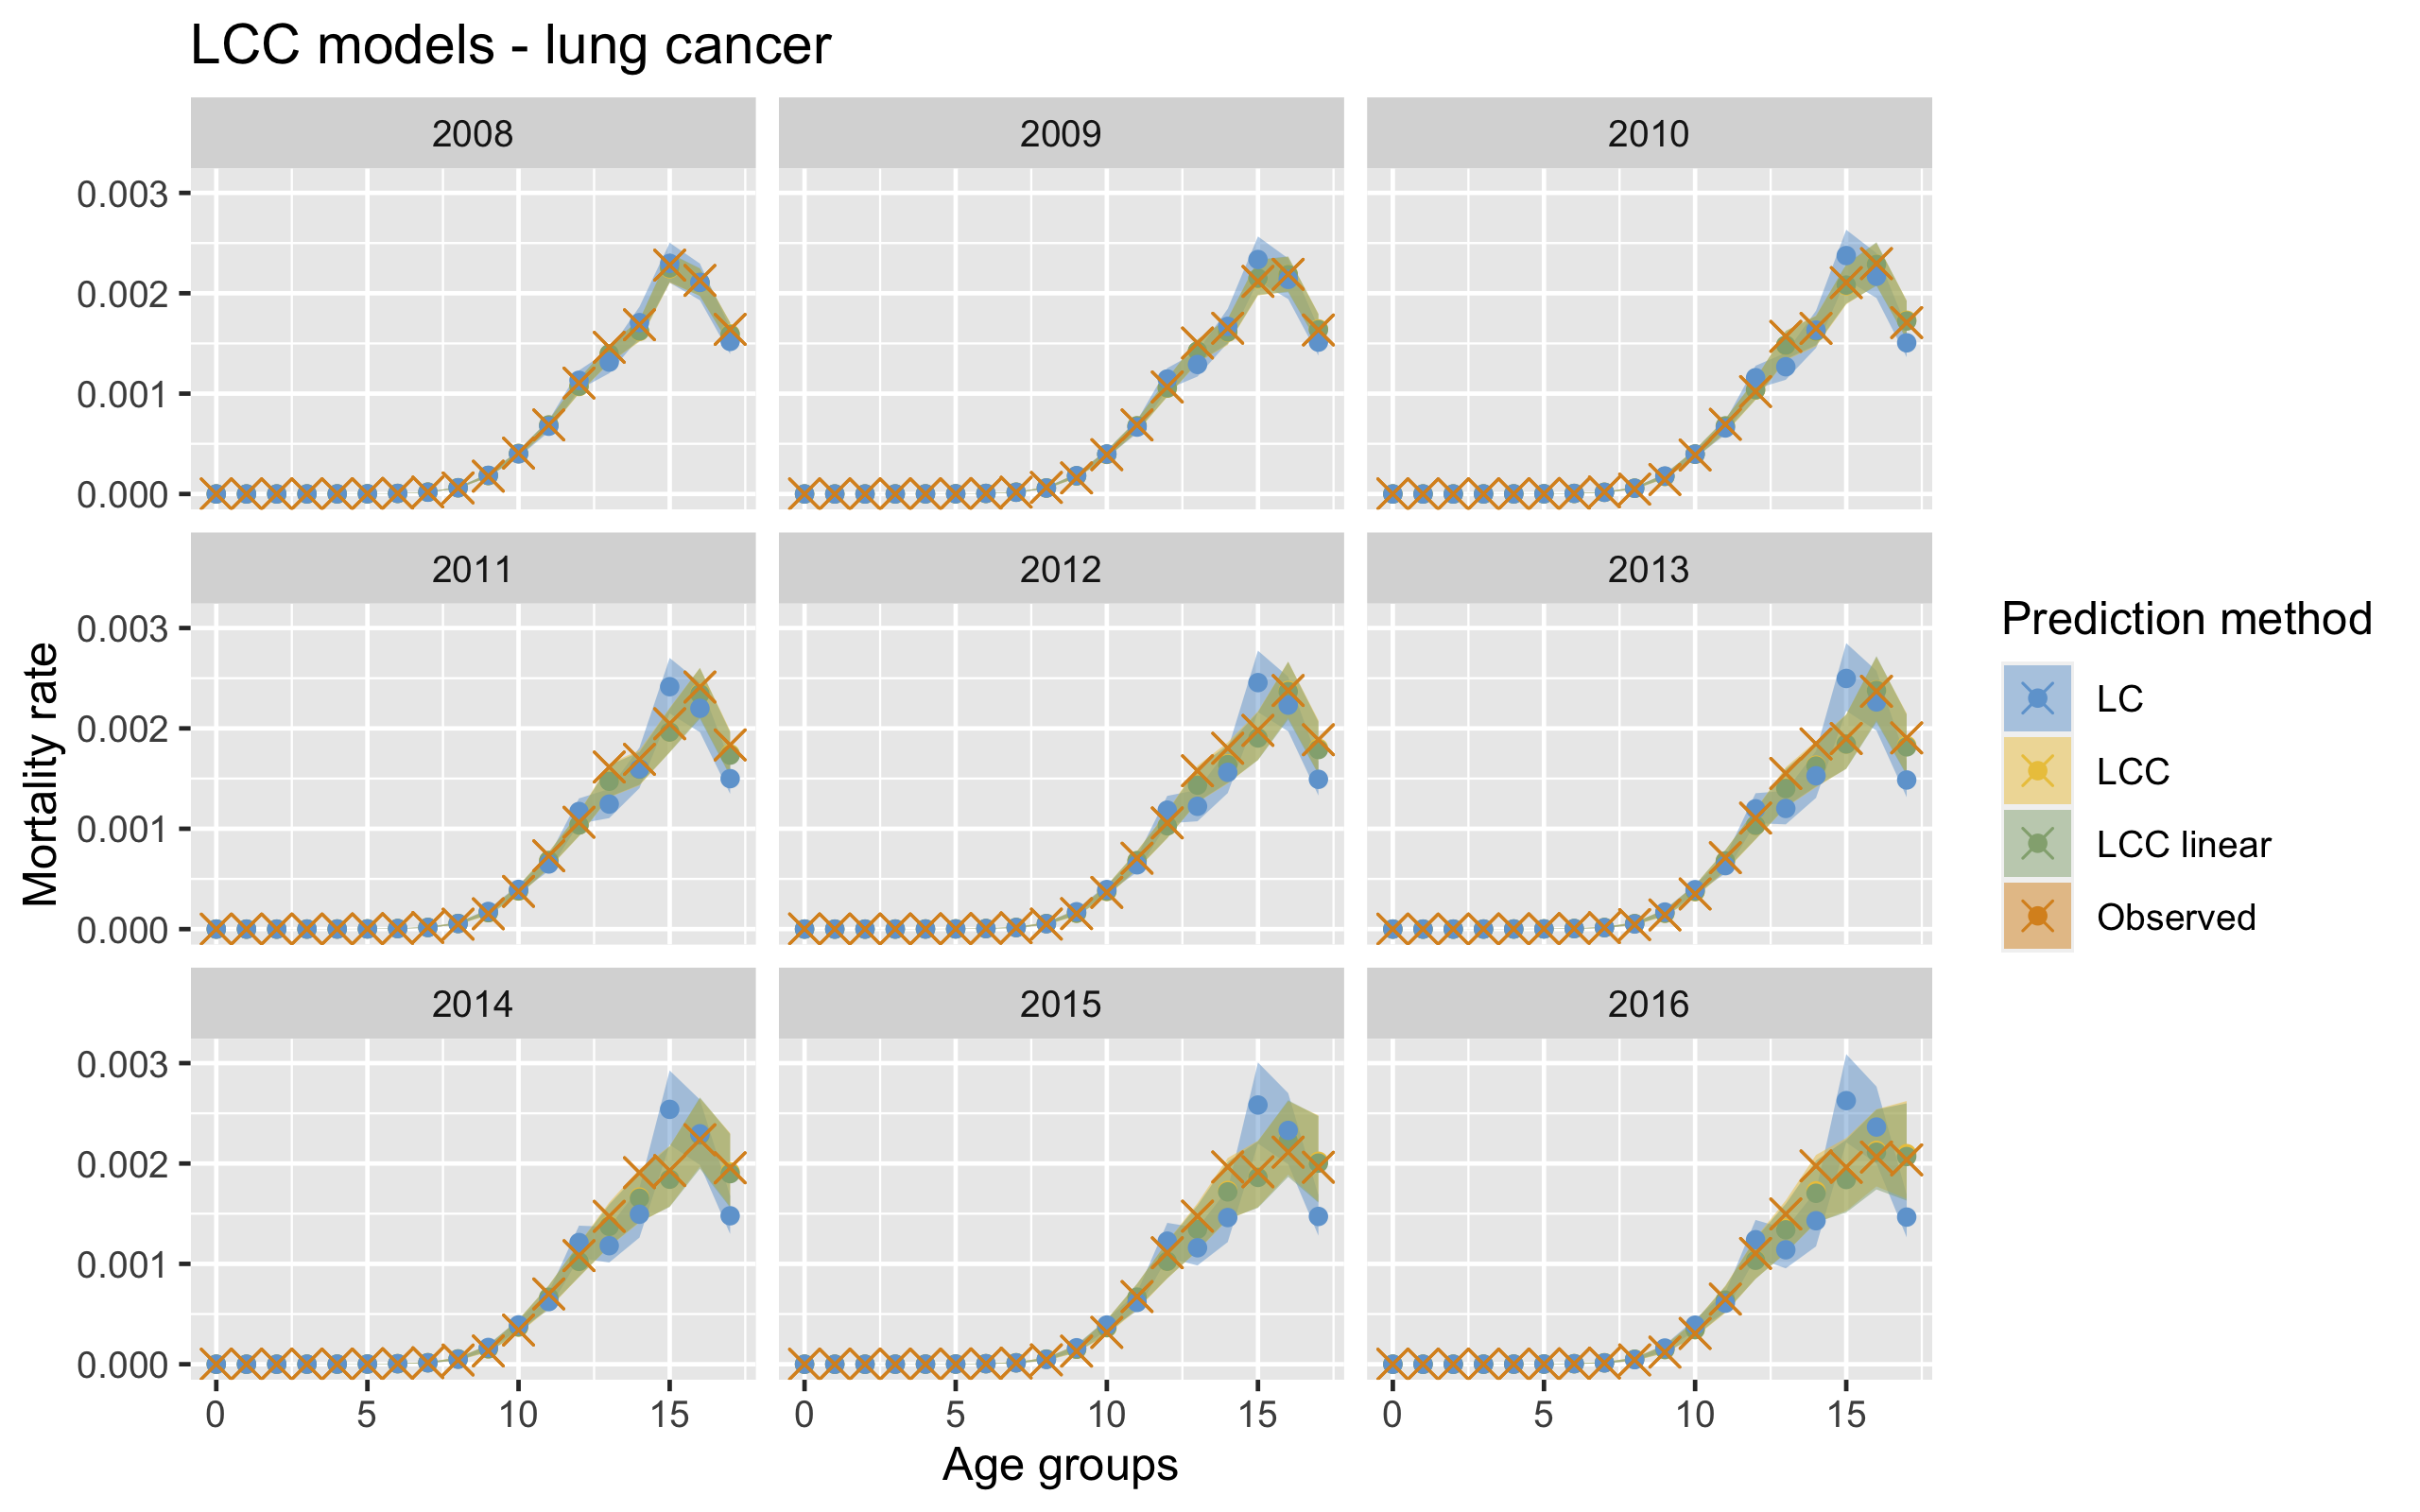
\includegraphics[width=\linewidth]{real-data/real-data-univariate/Figures/univariate-LCC-by-age-lung.png}
    \end{subfigure}
    \begin{subfigure}[b]{.45\linewidth}
        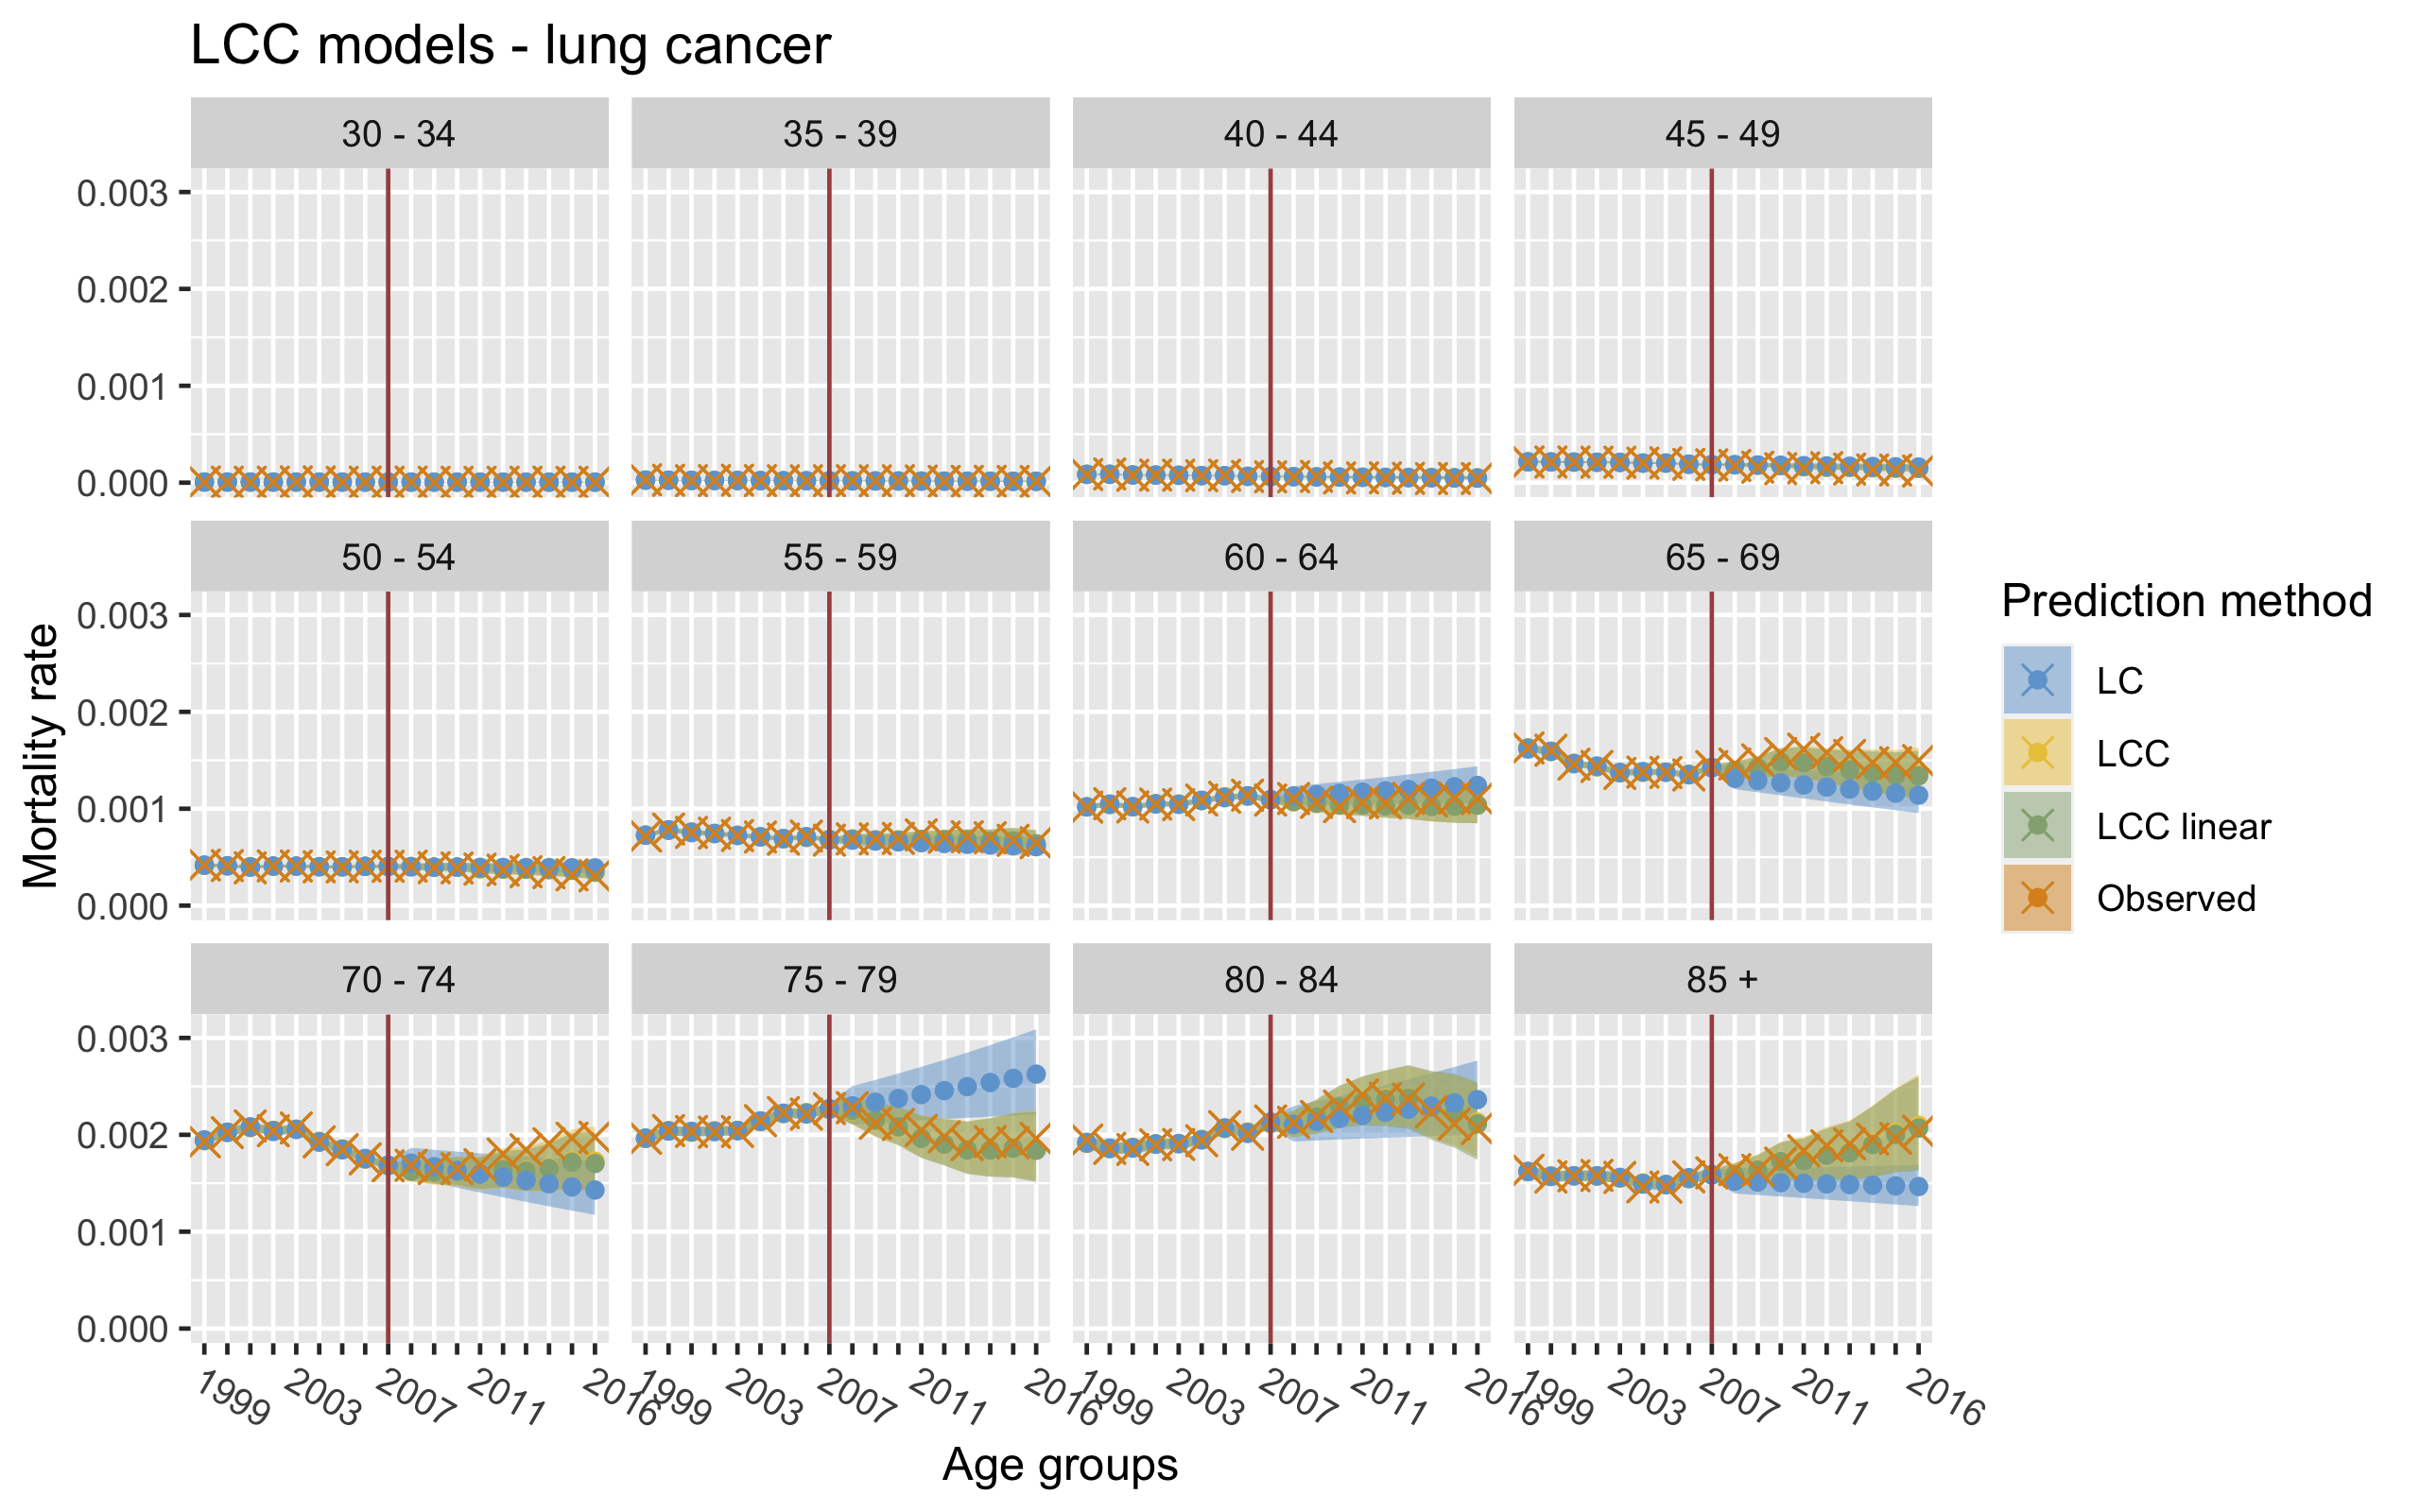
\includegraphics[width=\linewidth]{real-data/real-data-univariate/Figures/univariate-LCC-by-period-lung.png}
    \end{subfigure}
    \caption{The Lee-Carter types of models predicting lung cancer}
    \label{fig:uv-LCC-lung}
\end{figure}

\begin{figure}[h!]
    \centering
    \begin{subfigure}[b]{.45\linewidth}
        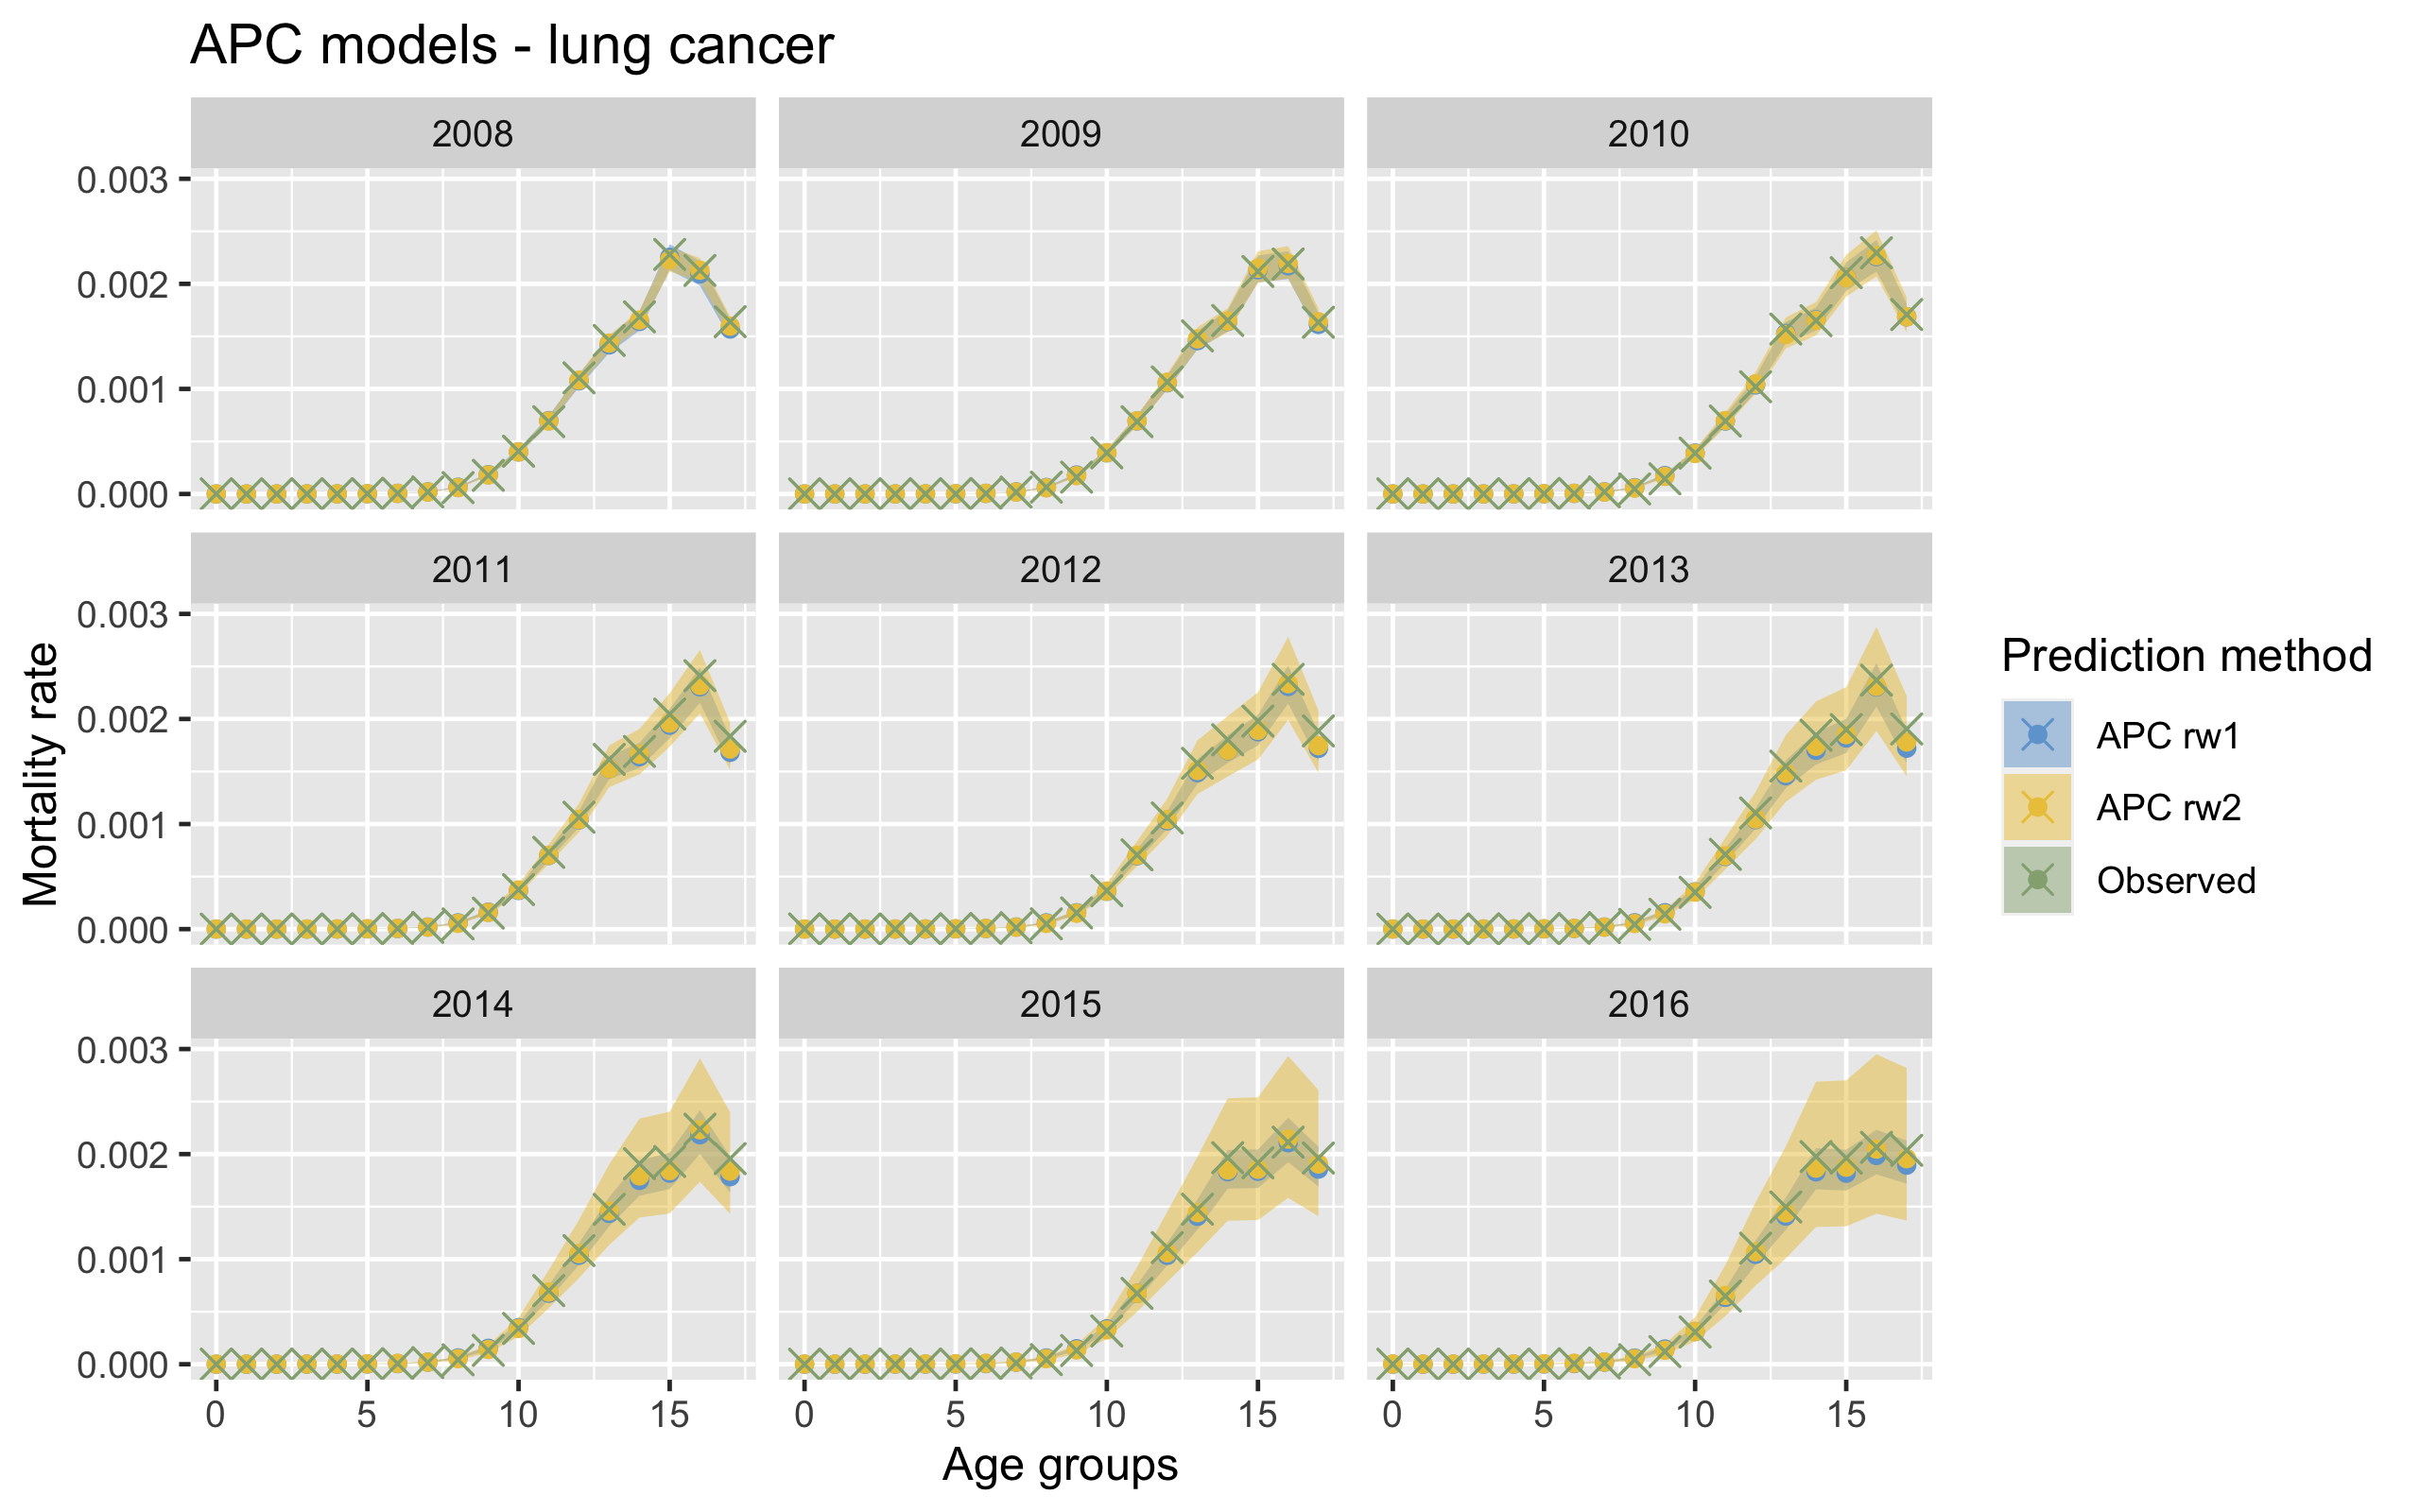
\includegraphics[width=\linewidth]{real-data/real-data-univariate/Figures/univariate-APC-by-age-lung.png}
    \end{subfigure}
    \begin{subfigure}[b]{.45\linewidth}
        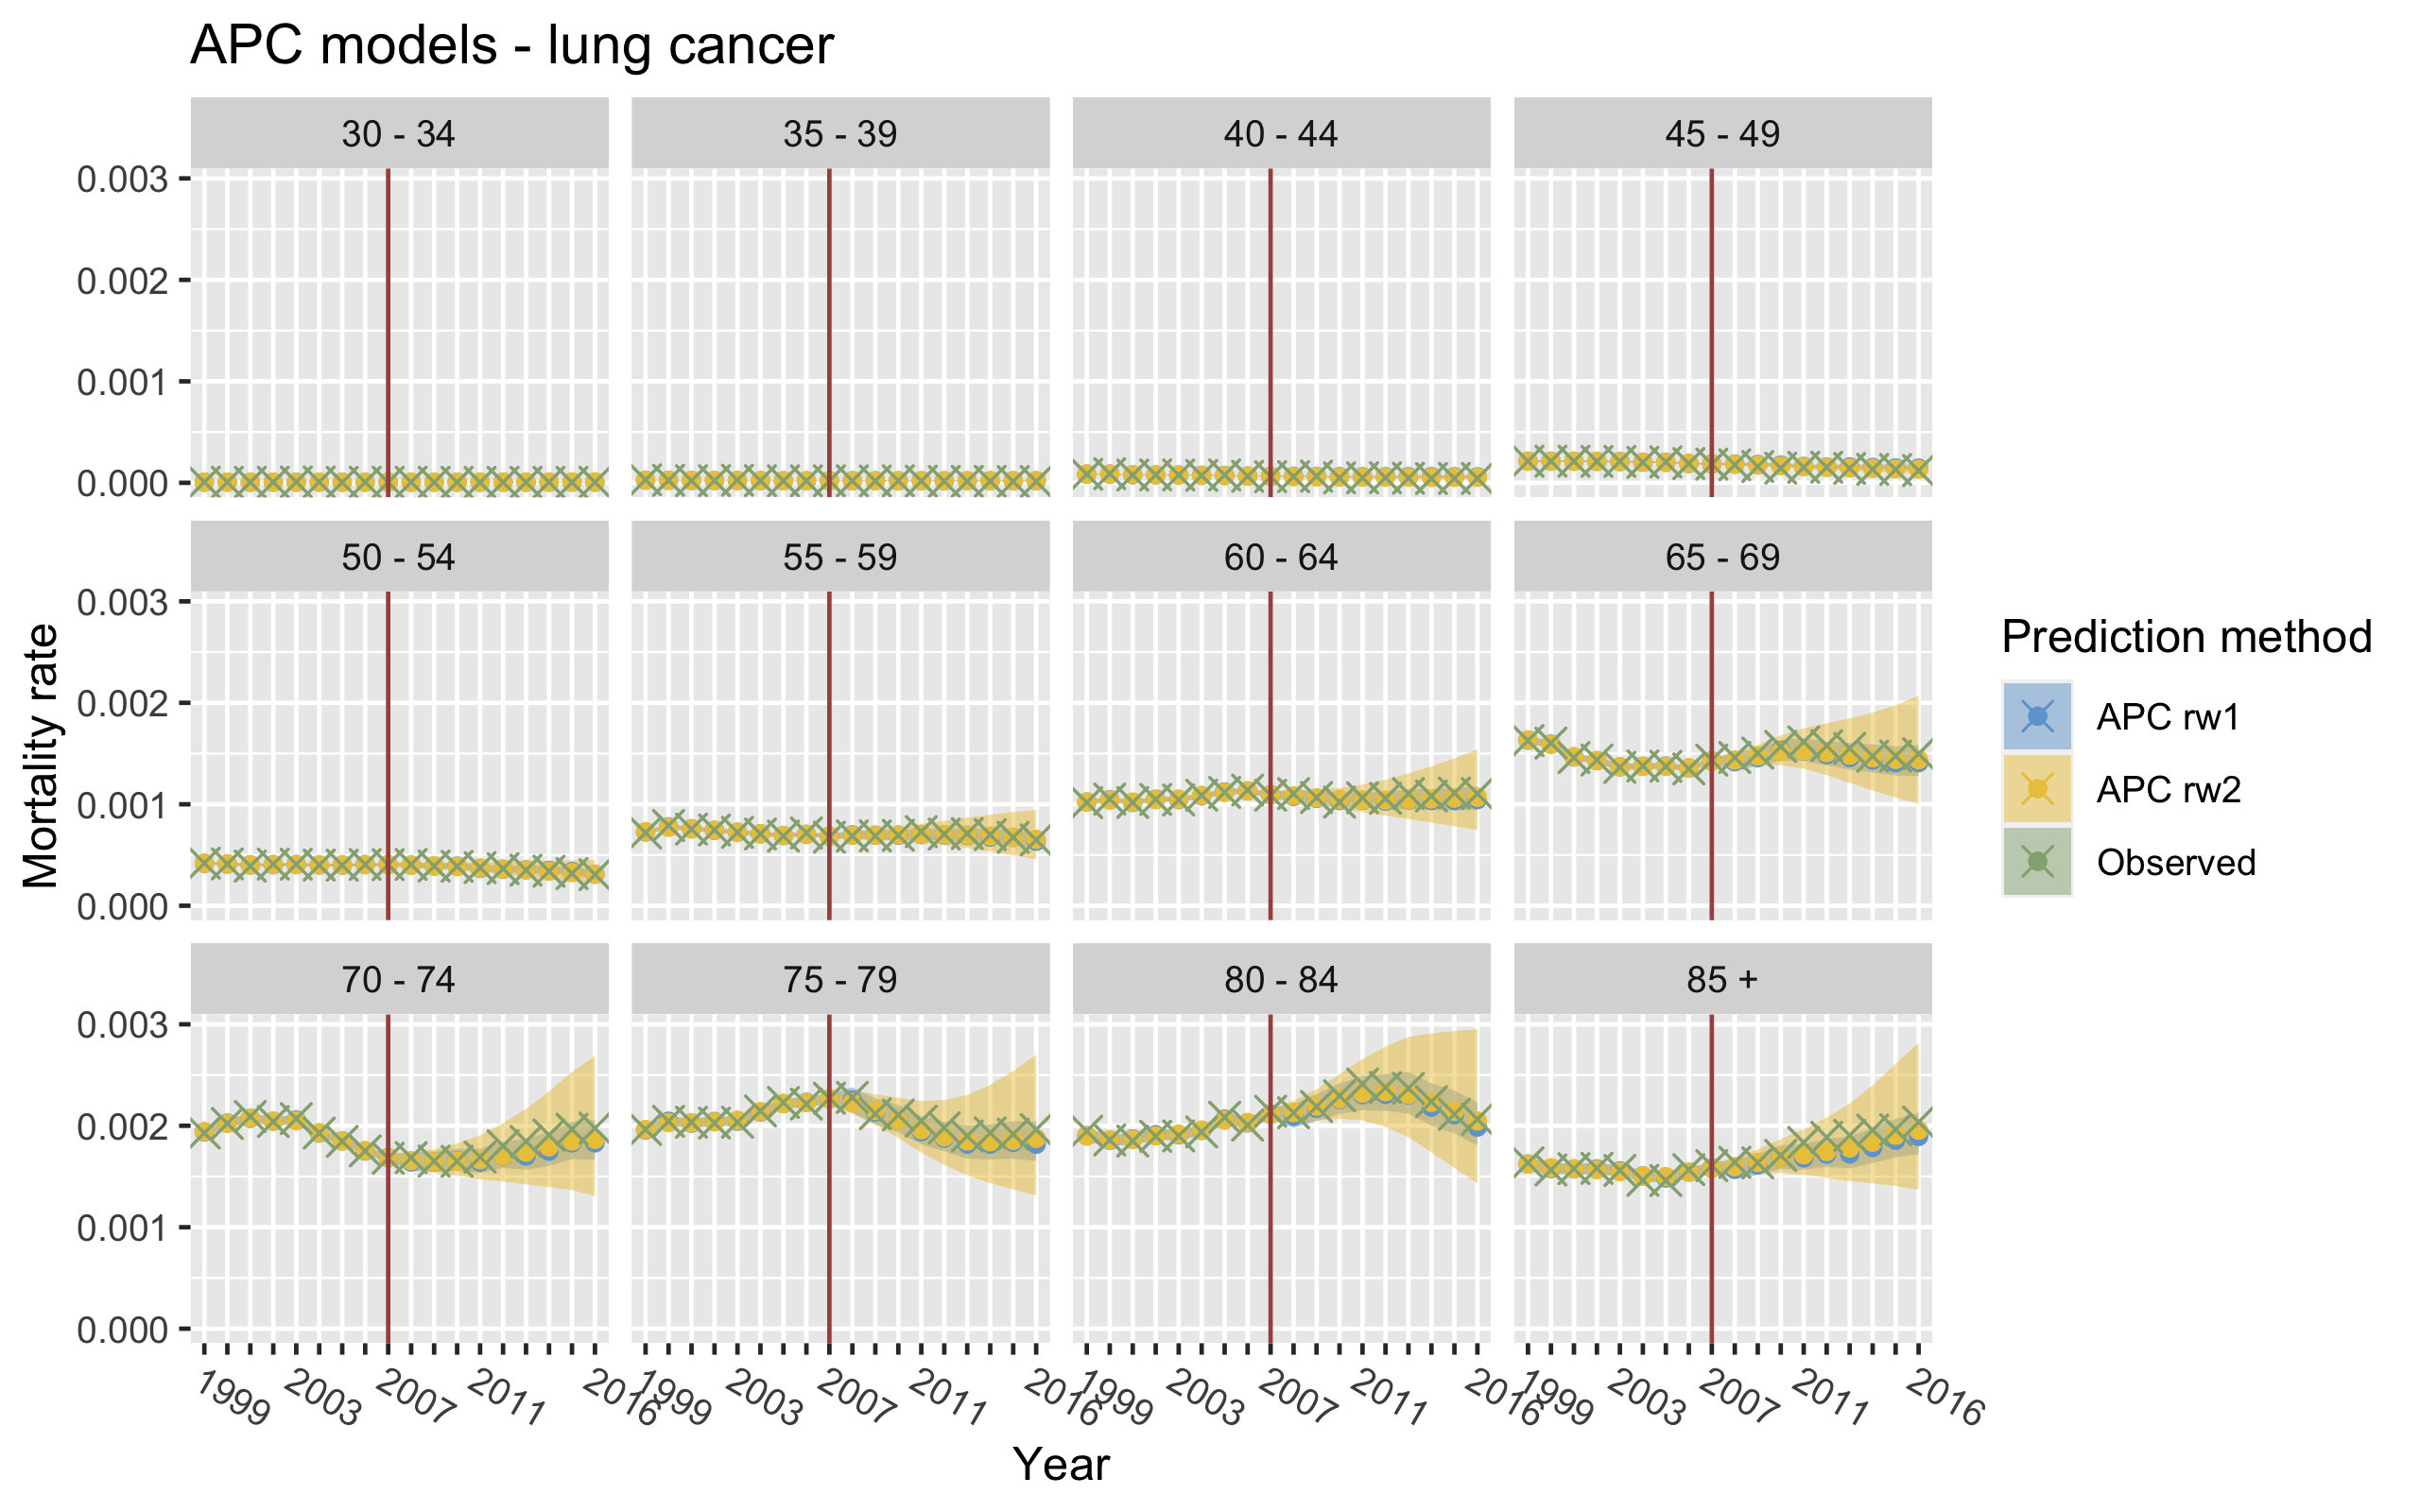
\includegraphics[width=\linewidth]{real-data/real-data-univariate/Figures/univariate-APC-by-period-lung.png}
    \end{subfigure}
    \caption{The APC types of models predicting lung cancer}
    \label{fig:uv-APC-lung}
\end{figure}

\begin{figure}[h!]
    \centering
    \begin{subfigure}[b]{.45\linewidth}
        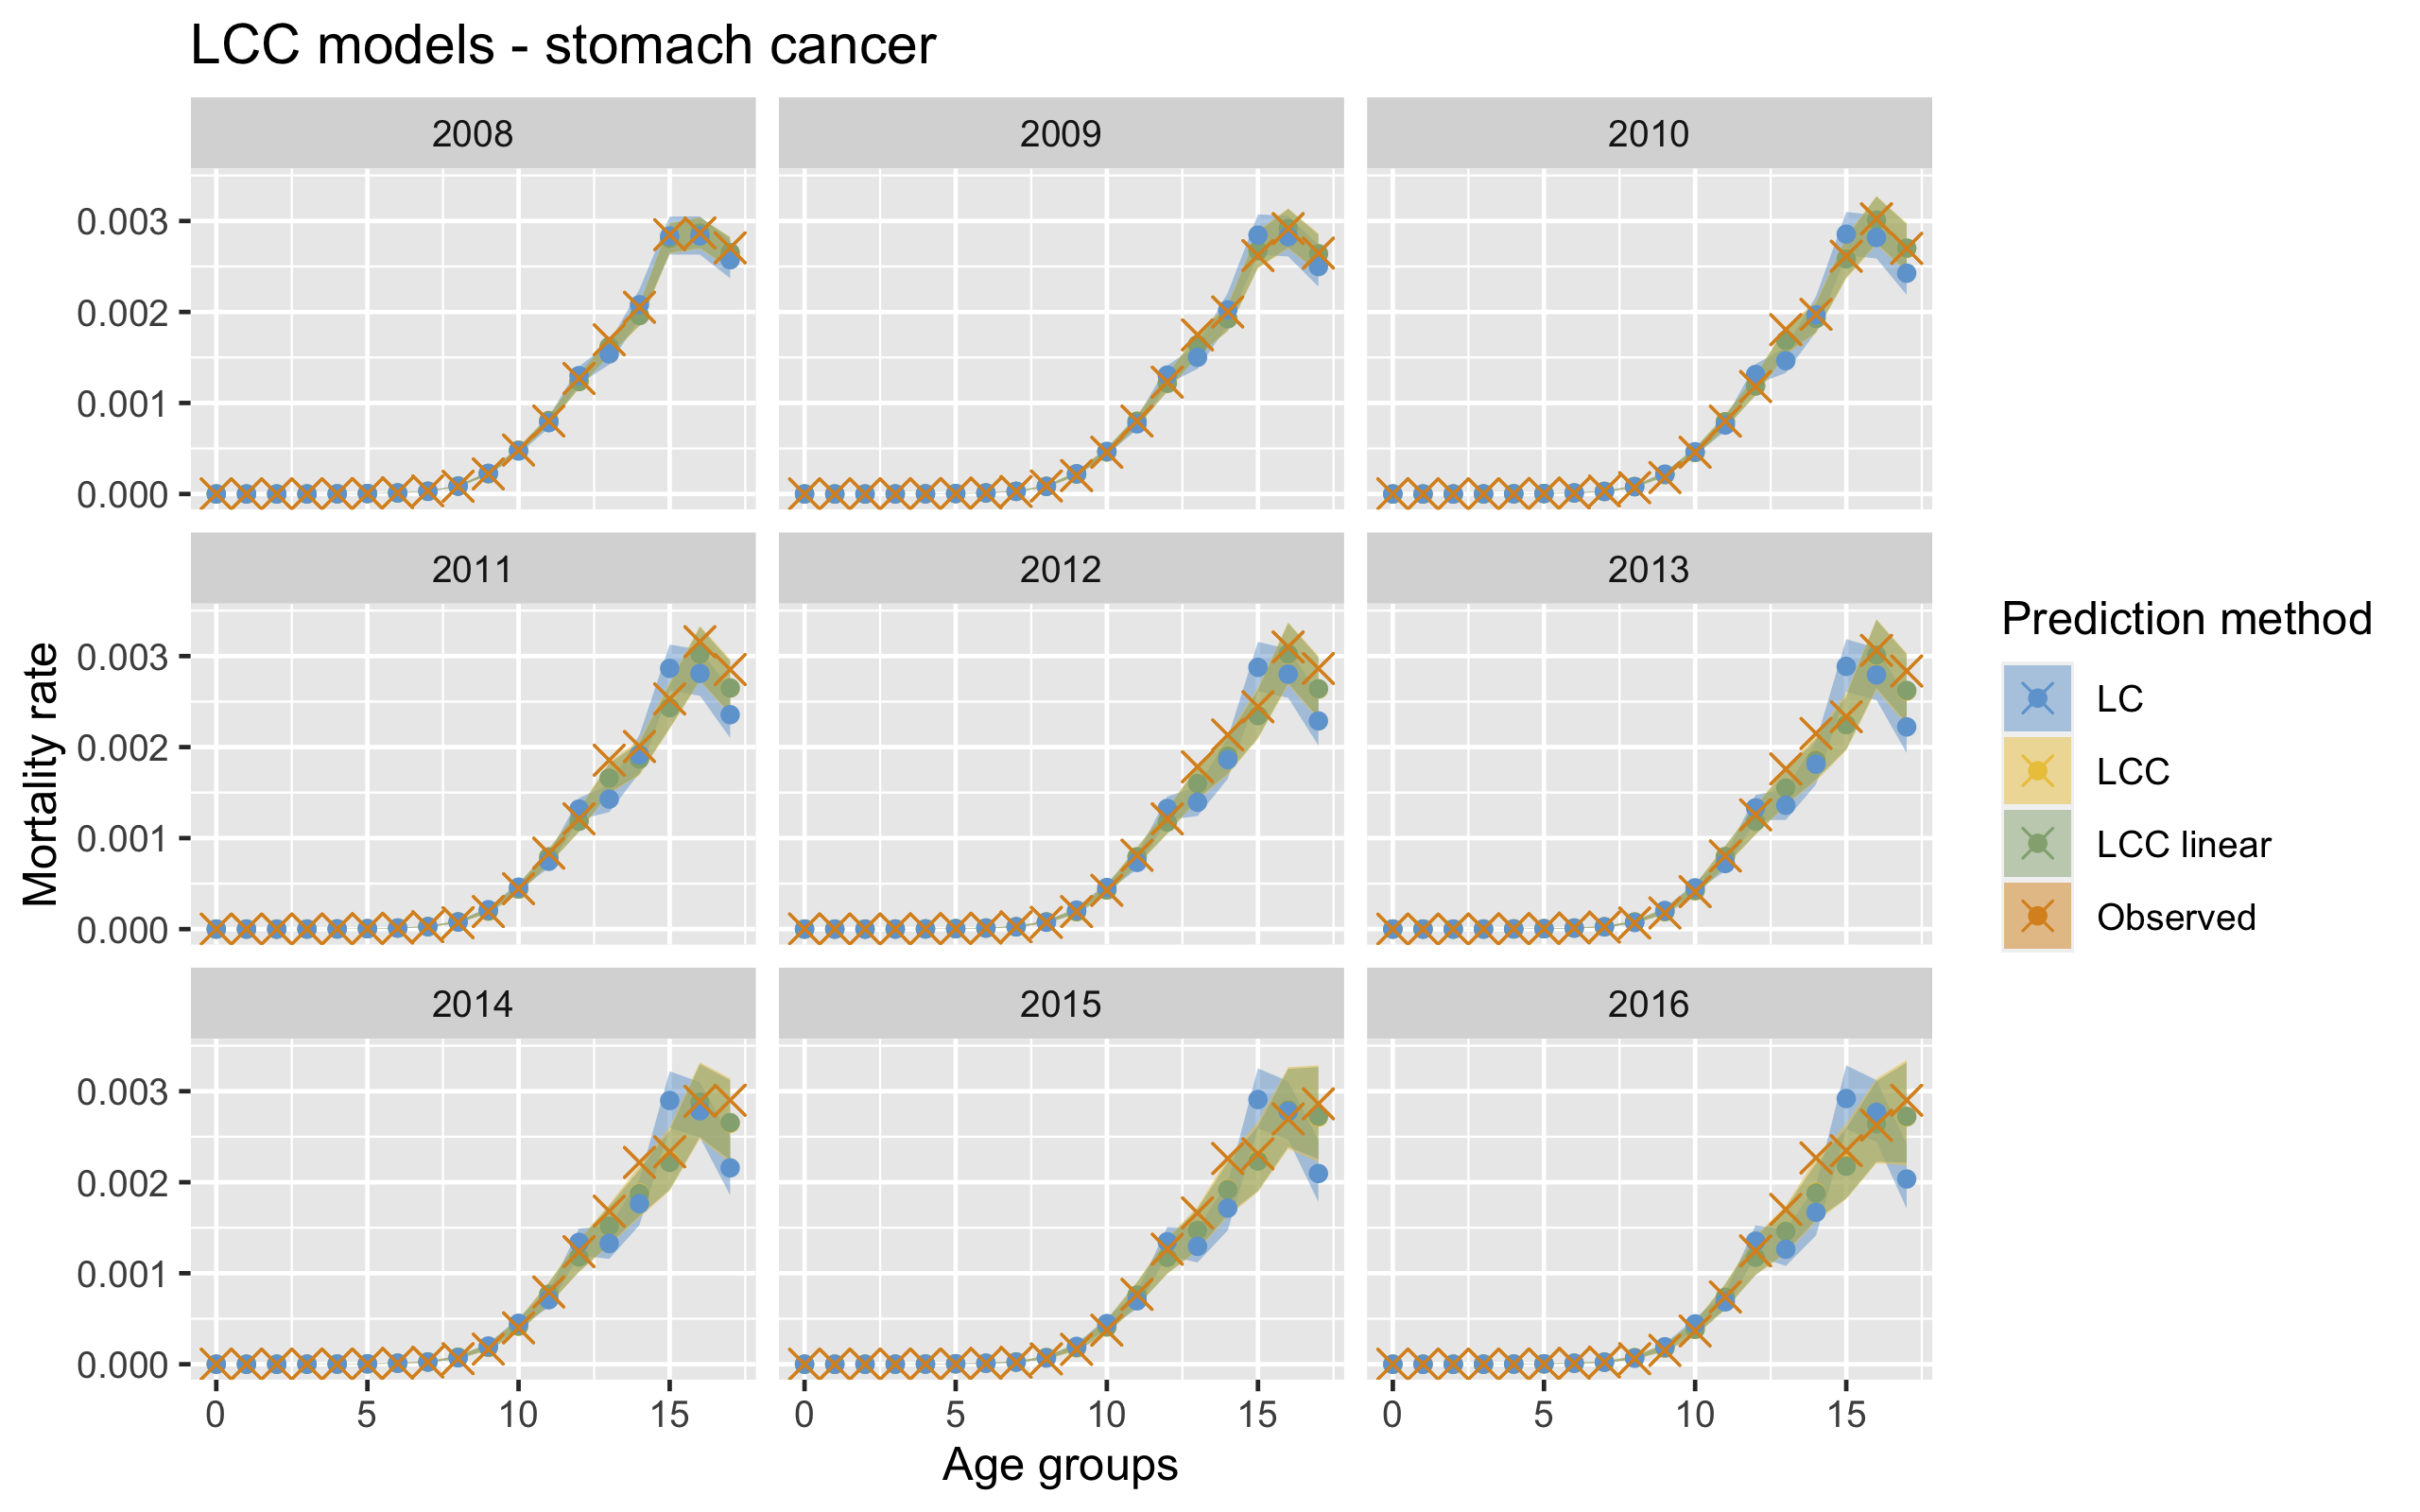
\includegraphics[width=\linewidth]{real-data/real-data-univariate/Figures/univariate-LCC-by-age-stomach.png}
    \end{subfigure}
    \begin{subfigure}[b]{.45\linewidth}
        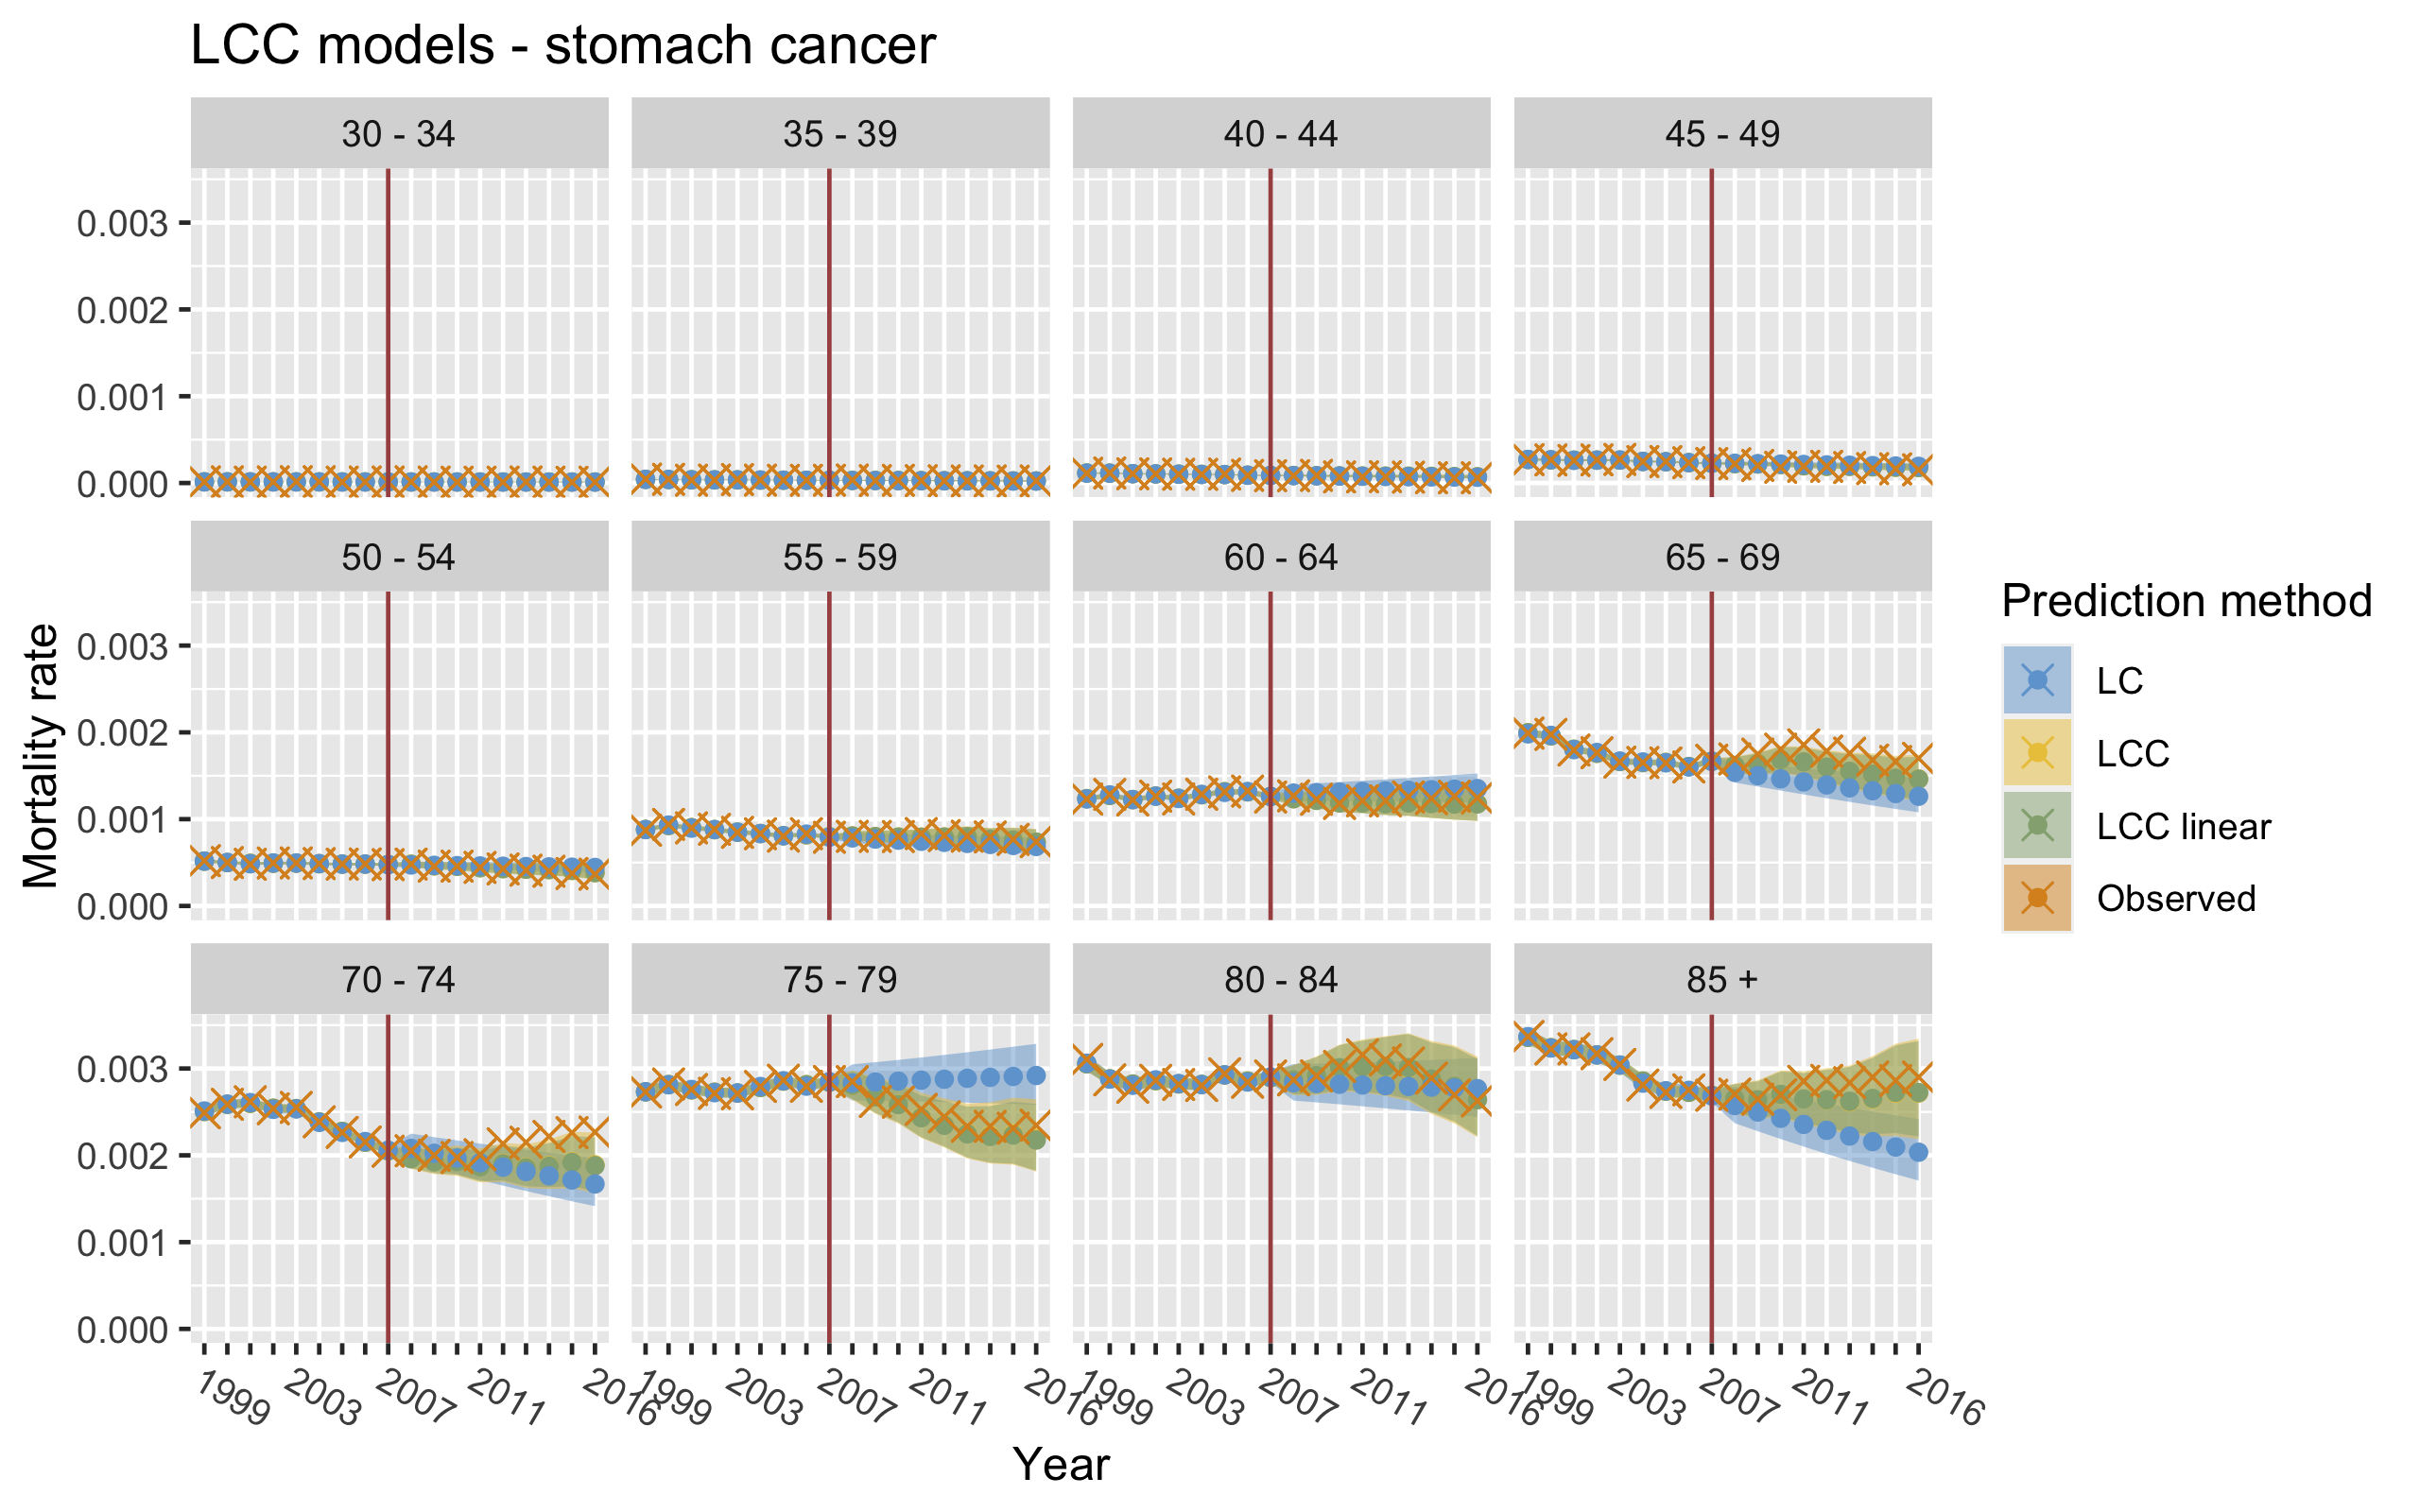
\includegraphics[width=\linewidth]{real-data/real-data-univariate/Figures/univariate-LCC-by-period-stomach.png}
    \end{subfigure}
    \caption{The Lee-Carter types of models predicting stomach cancer}
    \label{fig:uv-LCC-stomach}
\end{figure}

\begin{figure}[h!]
    \centering
    \begin{subfigure}[b]{.45\linewidth}
        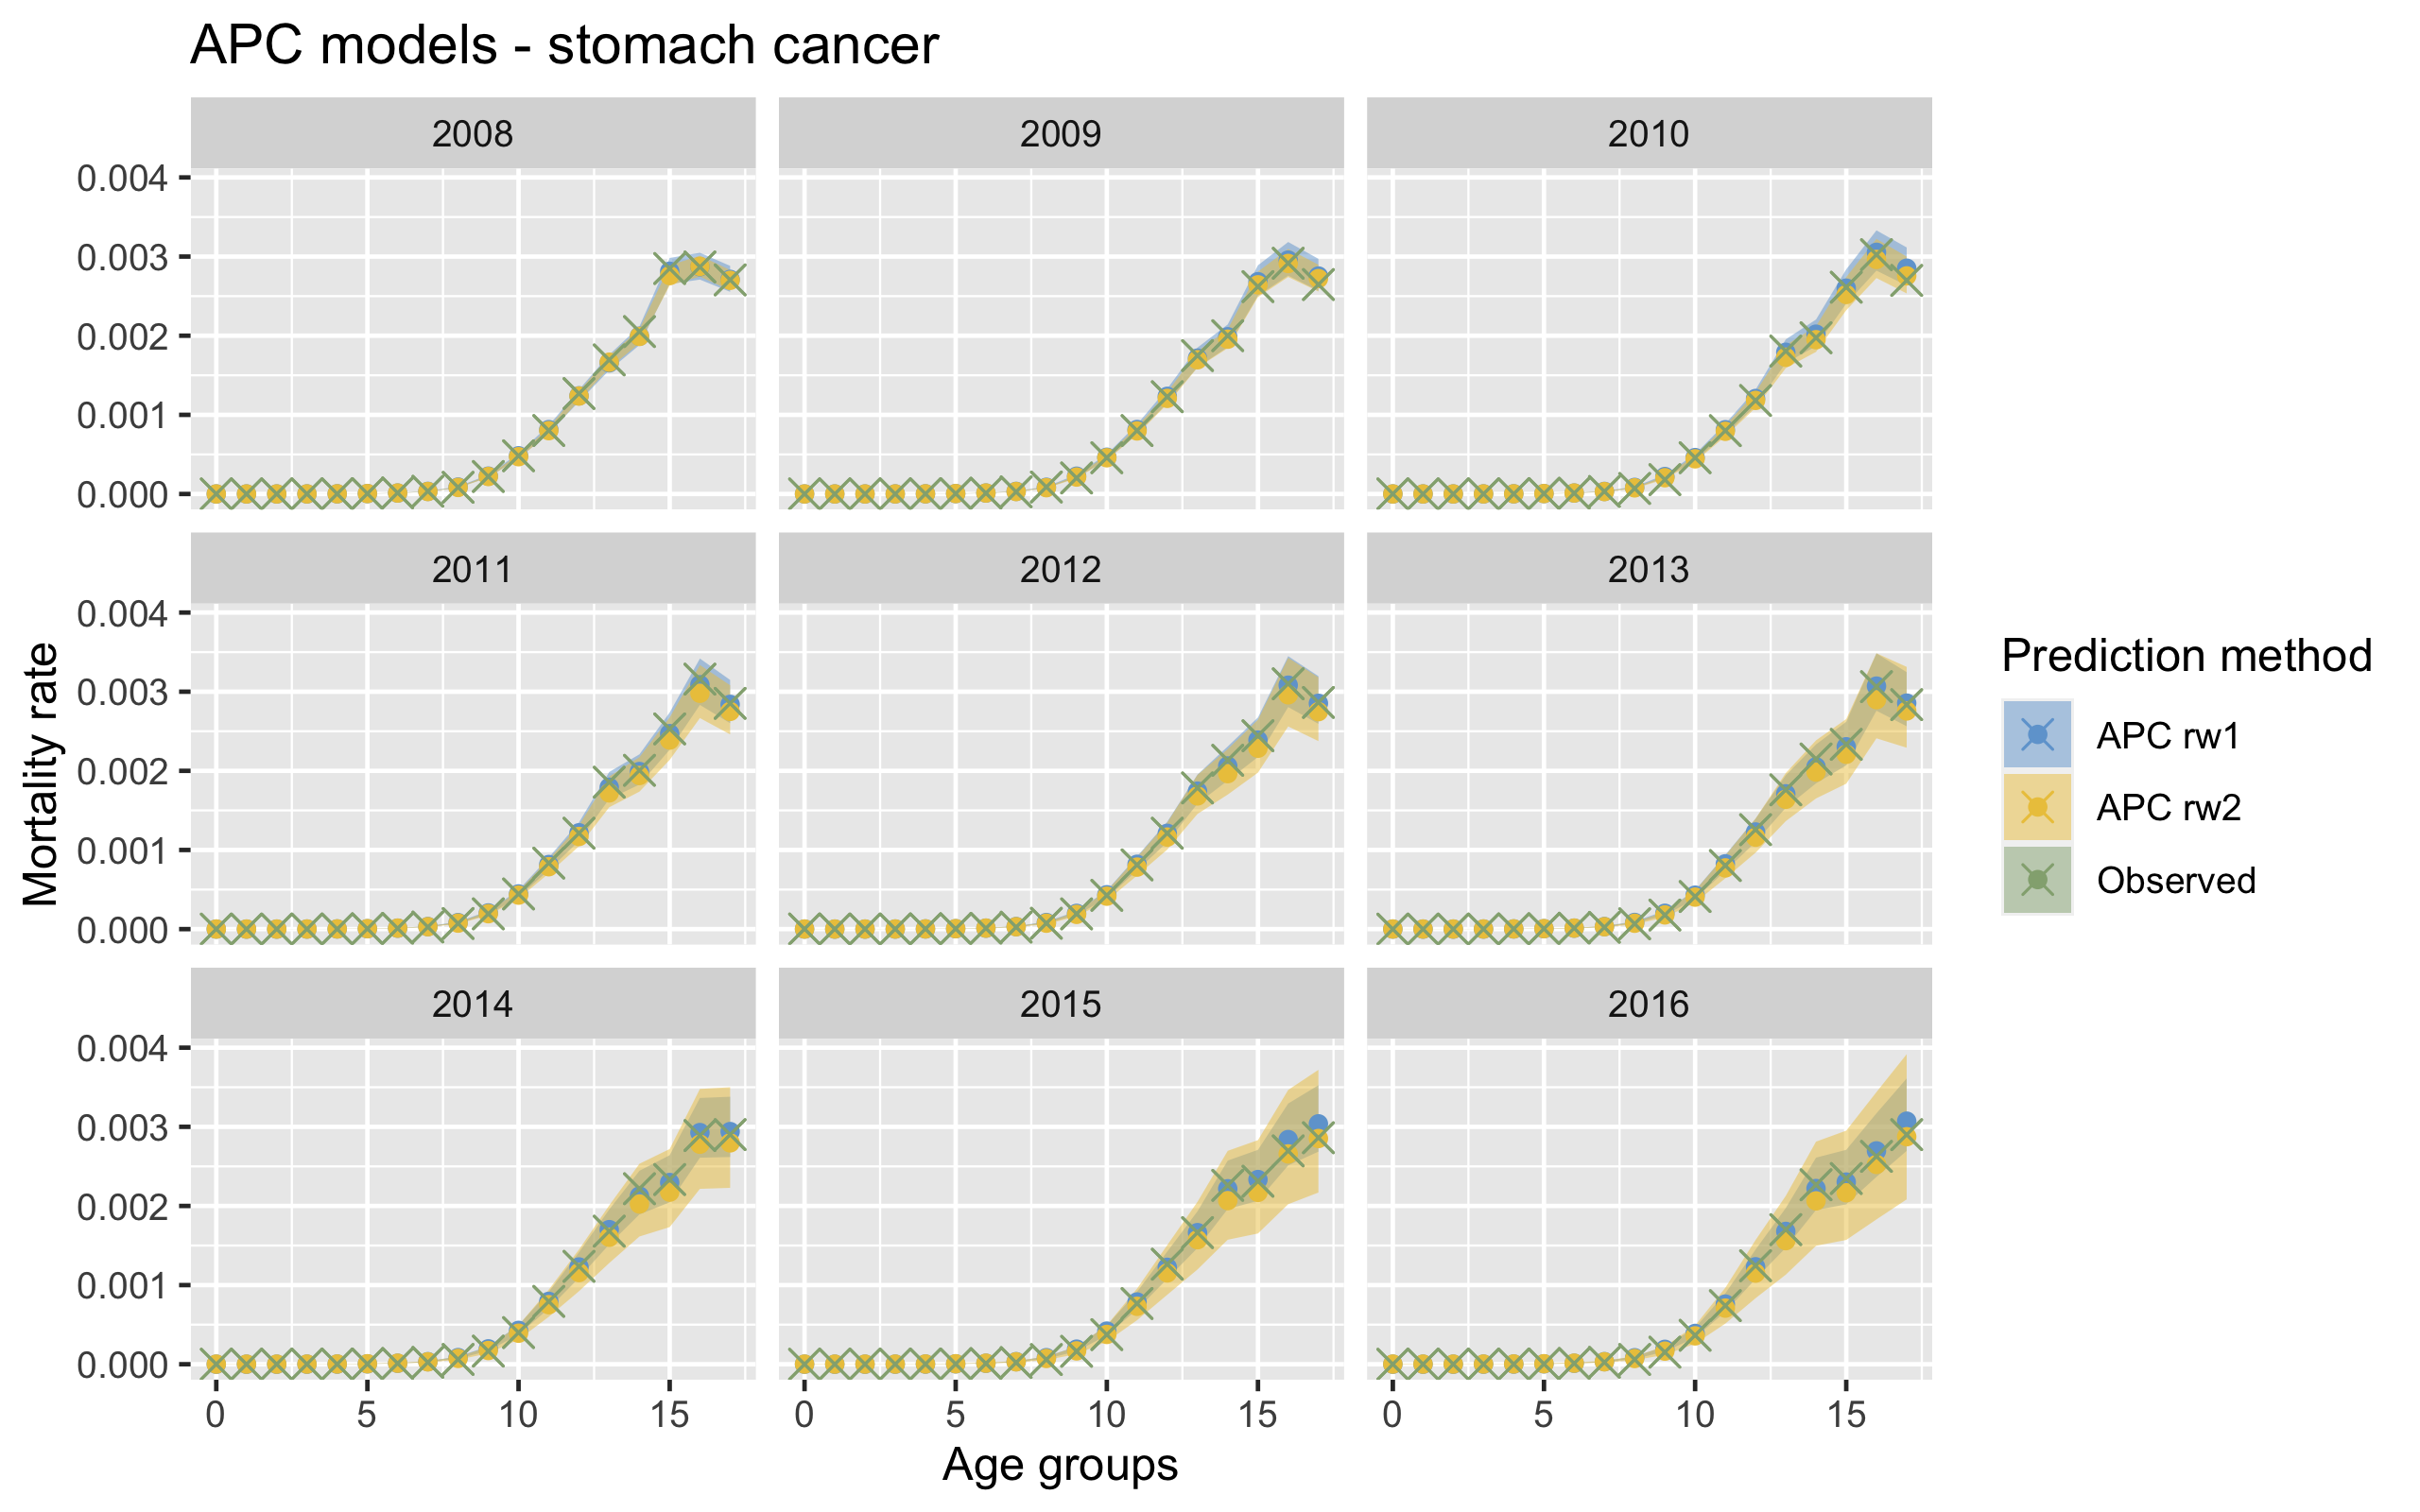
\includegraphics[width=\linewidth]{real-data/real-data-univariate/Figures/univariate-APC-by-age-stomach.png}
    \end{subfigure}
    \begin{subfigure}[b]{.45\linewidth}
        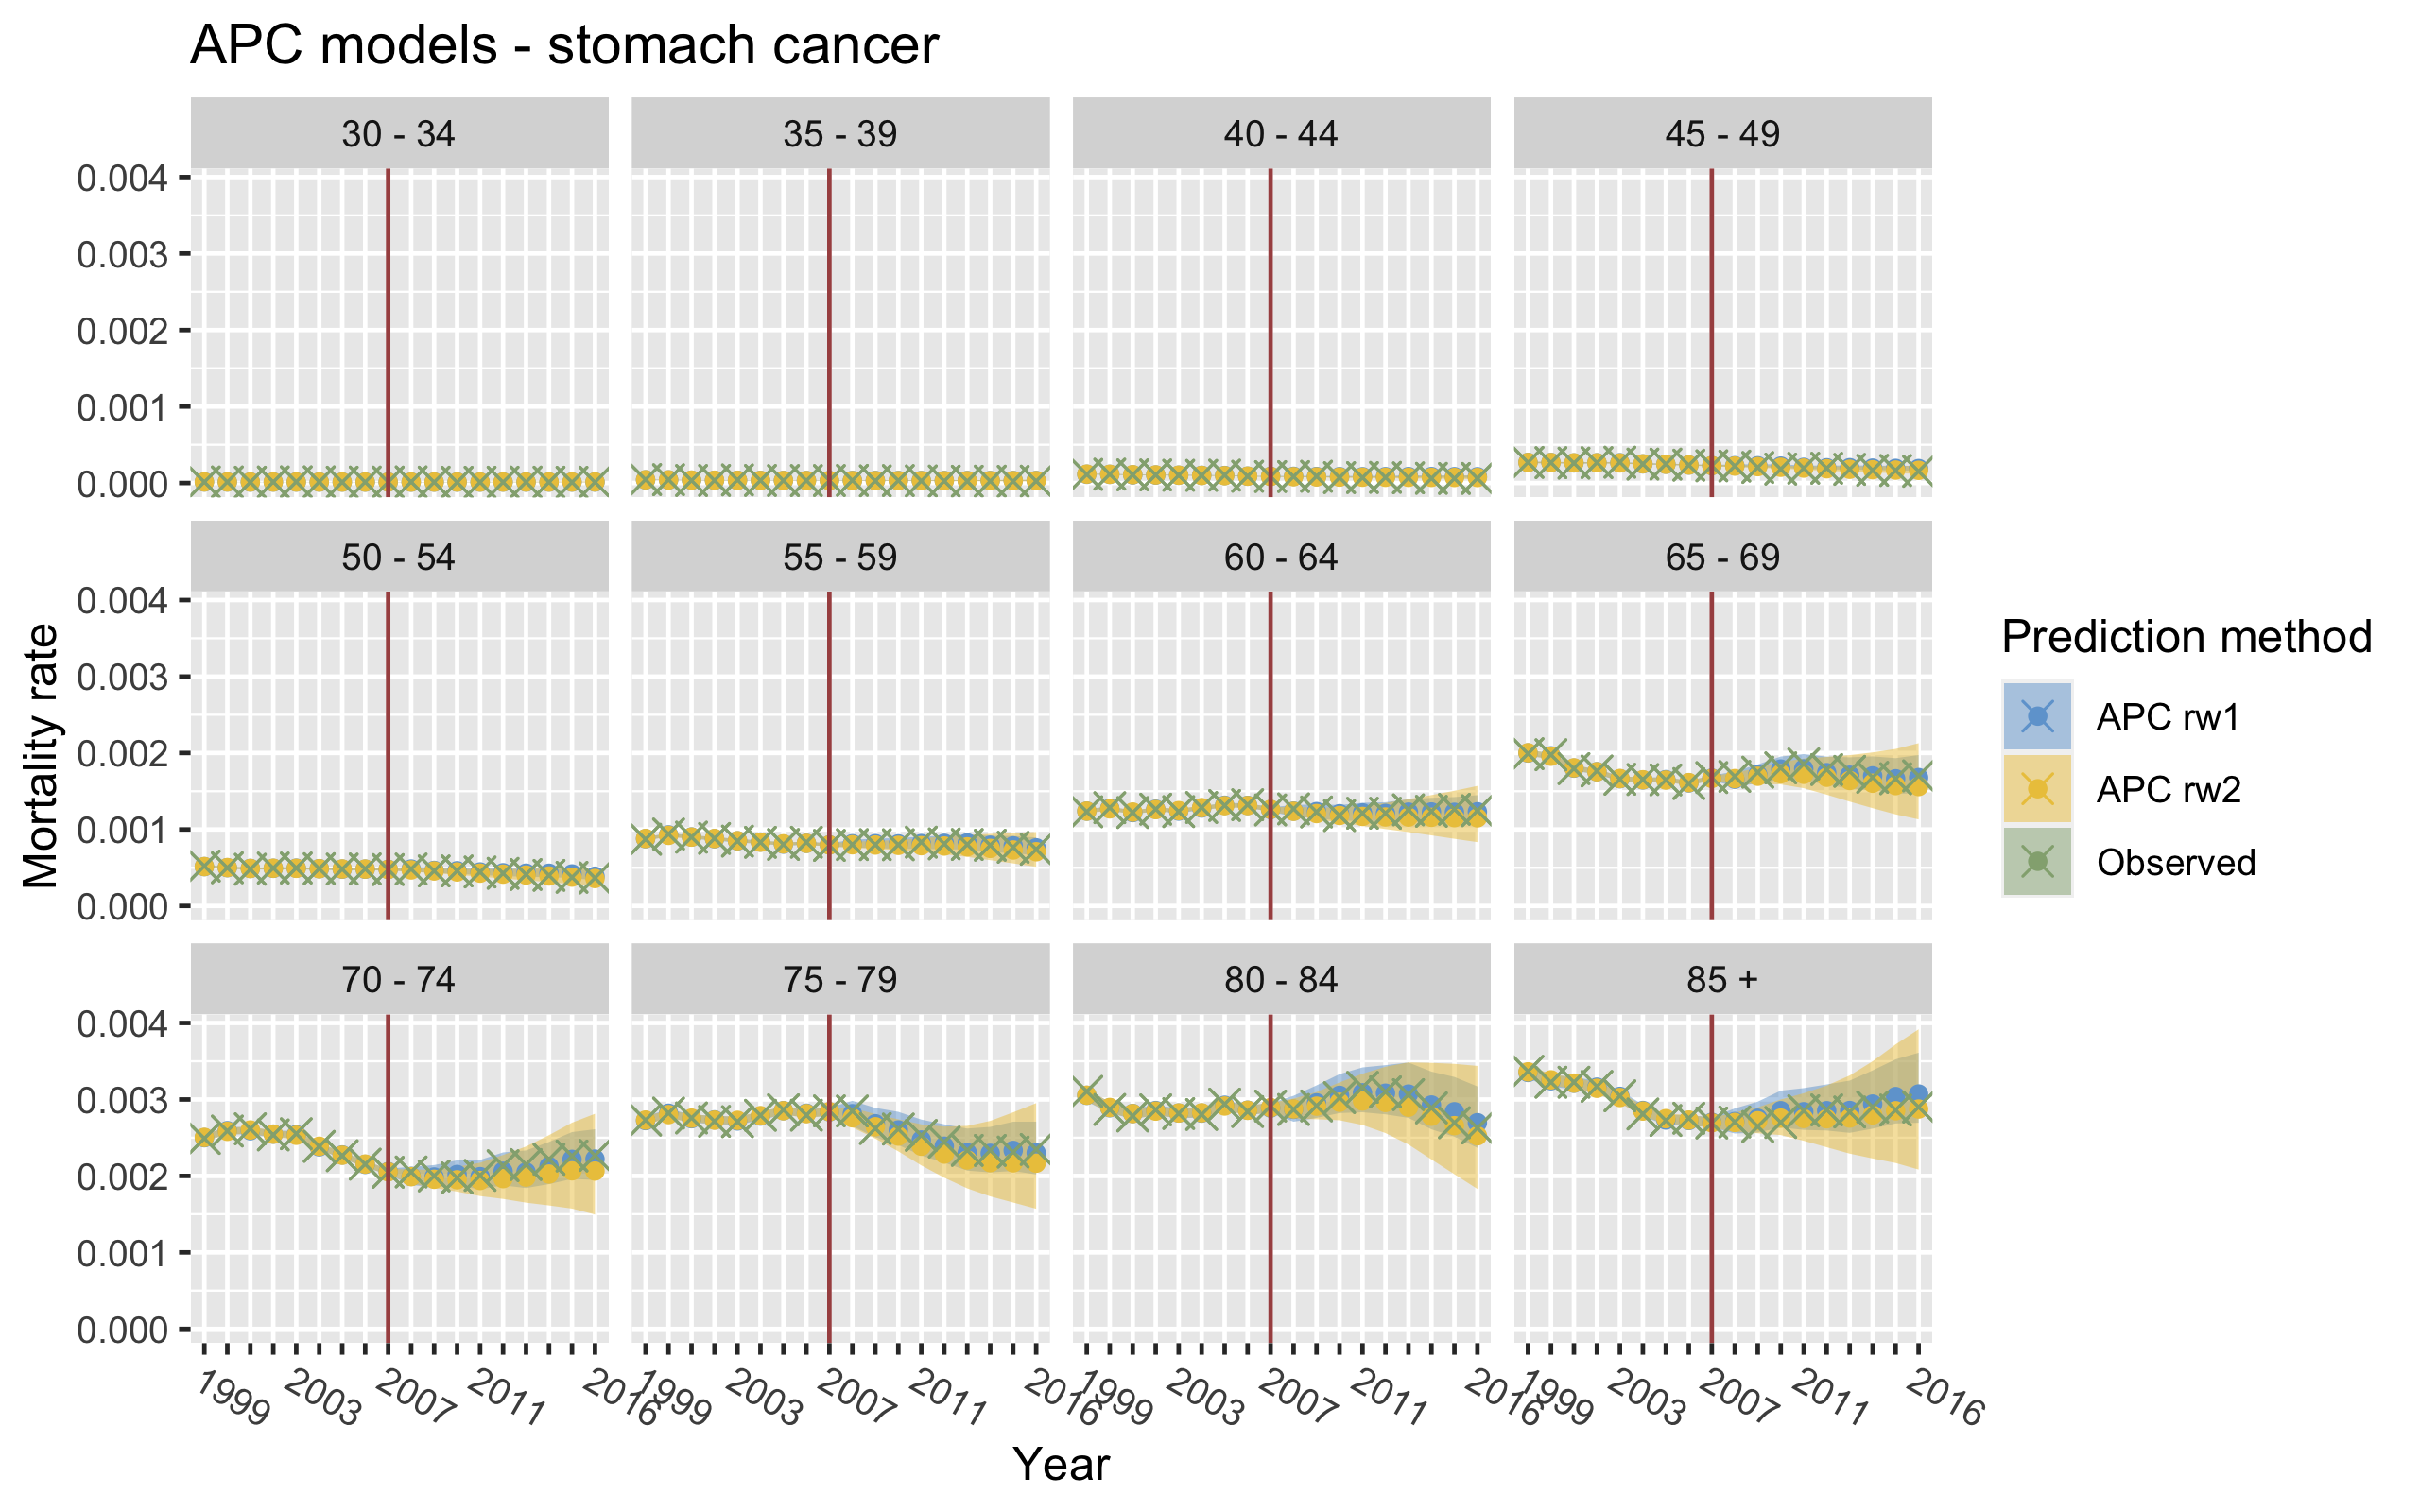
\includegraphics[width=\linewidth]{real-data/real-data-univariate/Figures/univariate-APC-by-period-stomach.png}
    \end{subfigure}
    \caption{The APC types of models predicting stomach cancer}
    \label{fig:uv-APC-stomach}
\end{figure}

Figures \ref{fig:uv-LCC-lung} and \ref{fig:uv-APC-lung} display the prediction results for lung cancer mortality, using the Lee-Carter and the APC methods, respectively. We present the predictions for each predicted year, with age groups along the x-axis (the left-most image in the figures) and for each age group, with all years along the x-axis (right-most image in the figures). For the images where results are displayed by age groups, we only show the results for ages above 30. This is simply because the real and predicted mortality rates are very close to zero for younger ages, so these results are not very interesting. The score statistics for these results are displayed in Table \textcolor{myDarkGreen}{TODO}. Figures \ref{fig:uv-LCC-stomach} and \ref{fig:uv-APC-stomach} and Table \textcolor{myDarkGreen}{TODO} show the same results for predictions of stomach cancer mortality. 
\newpar
From Figures \ref{fig:uv-LCC-lung} and \ref{fig:uv-LCC-stomach} we observe that, for both lung and stomach cancer, the LCC and LCC-linear models perform significantly better than the LC-model. This difference is especially apparent for the older age groups. The LCC- and the LCC-linear models seem, from the plotted results, to give very similar, and quite good, predictions. These observations are confirmed by the score statistics in Table \textcolor{myDarkGreen}{TODO}. The MDSS for the LC-model is clearly higher than the MDSS for the LCC and the LCC-linear models, which is a clear indication that the LC-model performs worse than the others. \textcolor{myDarkGreen}{The LCC and the LCC-linear models have very similar score statistics. The MDSS for the LCC model is slightly lower than the MDSS for the LCC-linear model, both for lung and stomach cancer, indicating that the former gives better predictions. Since this was our original proposed model, and we do not seem to gain performance in prediction by omitting the non-linear period term $\kappa_t$, we keep this model in our following investigation. Still, we underline that it seems like most of the period-related variability in the mortality rates can be explained by a linear trend. }

For the two APC models, APC1 and APC2, it is less clear which model perform the best. Figures \ref{fig:uv-APC-lung} and \ref{fig:uv-APC-stomach} display the results from using the APC models to predict lung and stomach cancer mortality. Firstly, we note that both the APC1 and APC2 models seem to predict the mortality rates well, both for lung and stomach cancer. We observe that for both cancer types, the APC2 model produces predictions with wider prediction intervals than the APC1 model does. We also observe that the prediction intervals from the APC2 model is widening with more recent years (the predictions get less sharp further into the future). This tendency is not as clear for the APC1 model. For lung cancer mortality, we observe from Figure \ref{fig:uv-APC-lung} that the APC2 predictions might be slightly more accurate than the APC1 predictions. We especially see this tendency for older age groups. For stomach cancer however, we are not able to determine which of the models are more accurate just from looking at the plots in Figure \ref{fig:uv-APC-stomach}. \textcolor{myDarkGreen}{TODO: include tables and say something about how RW2 is preferred based on MDSS} 

\begin{figure}[h!]
    \centering
    \begin{subfigure}[b]{.45\linewidth}
        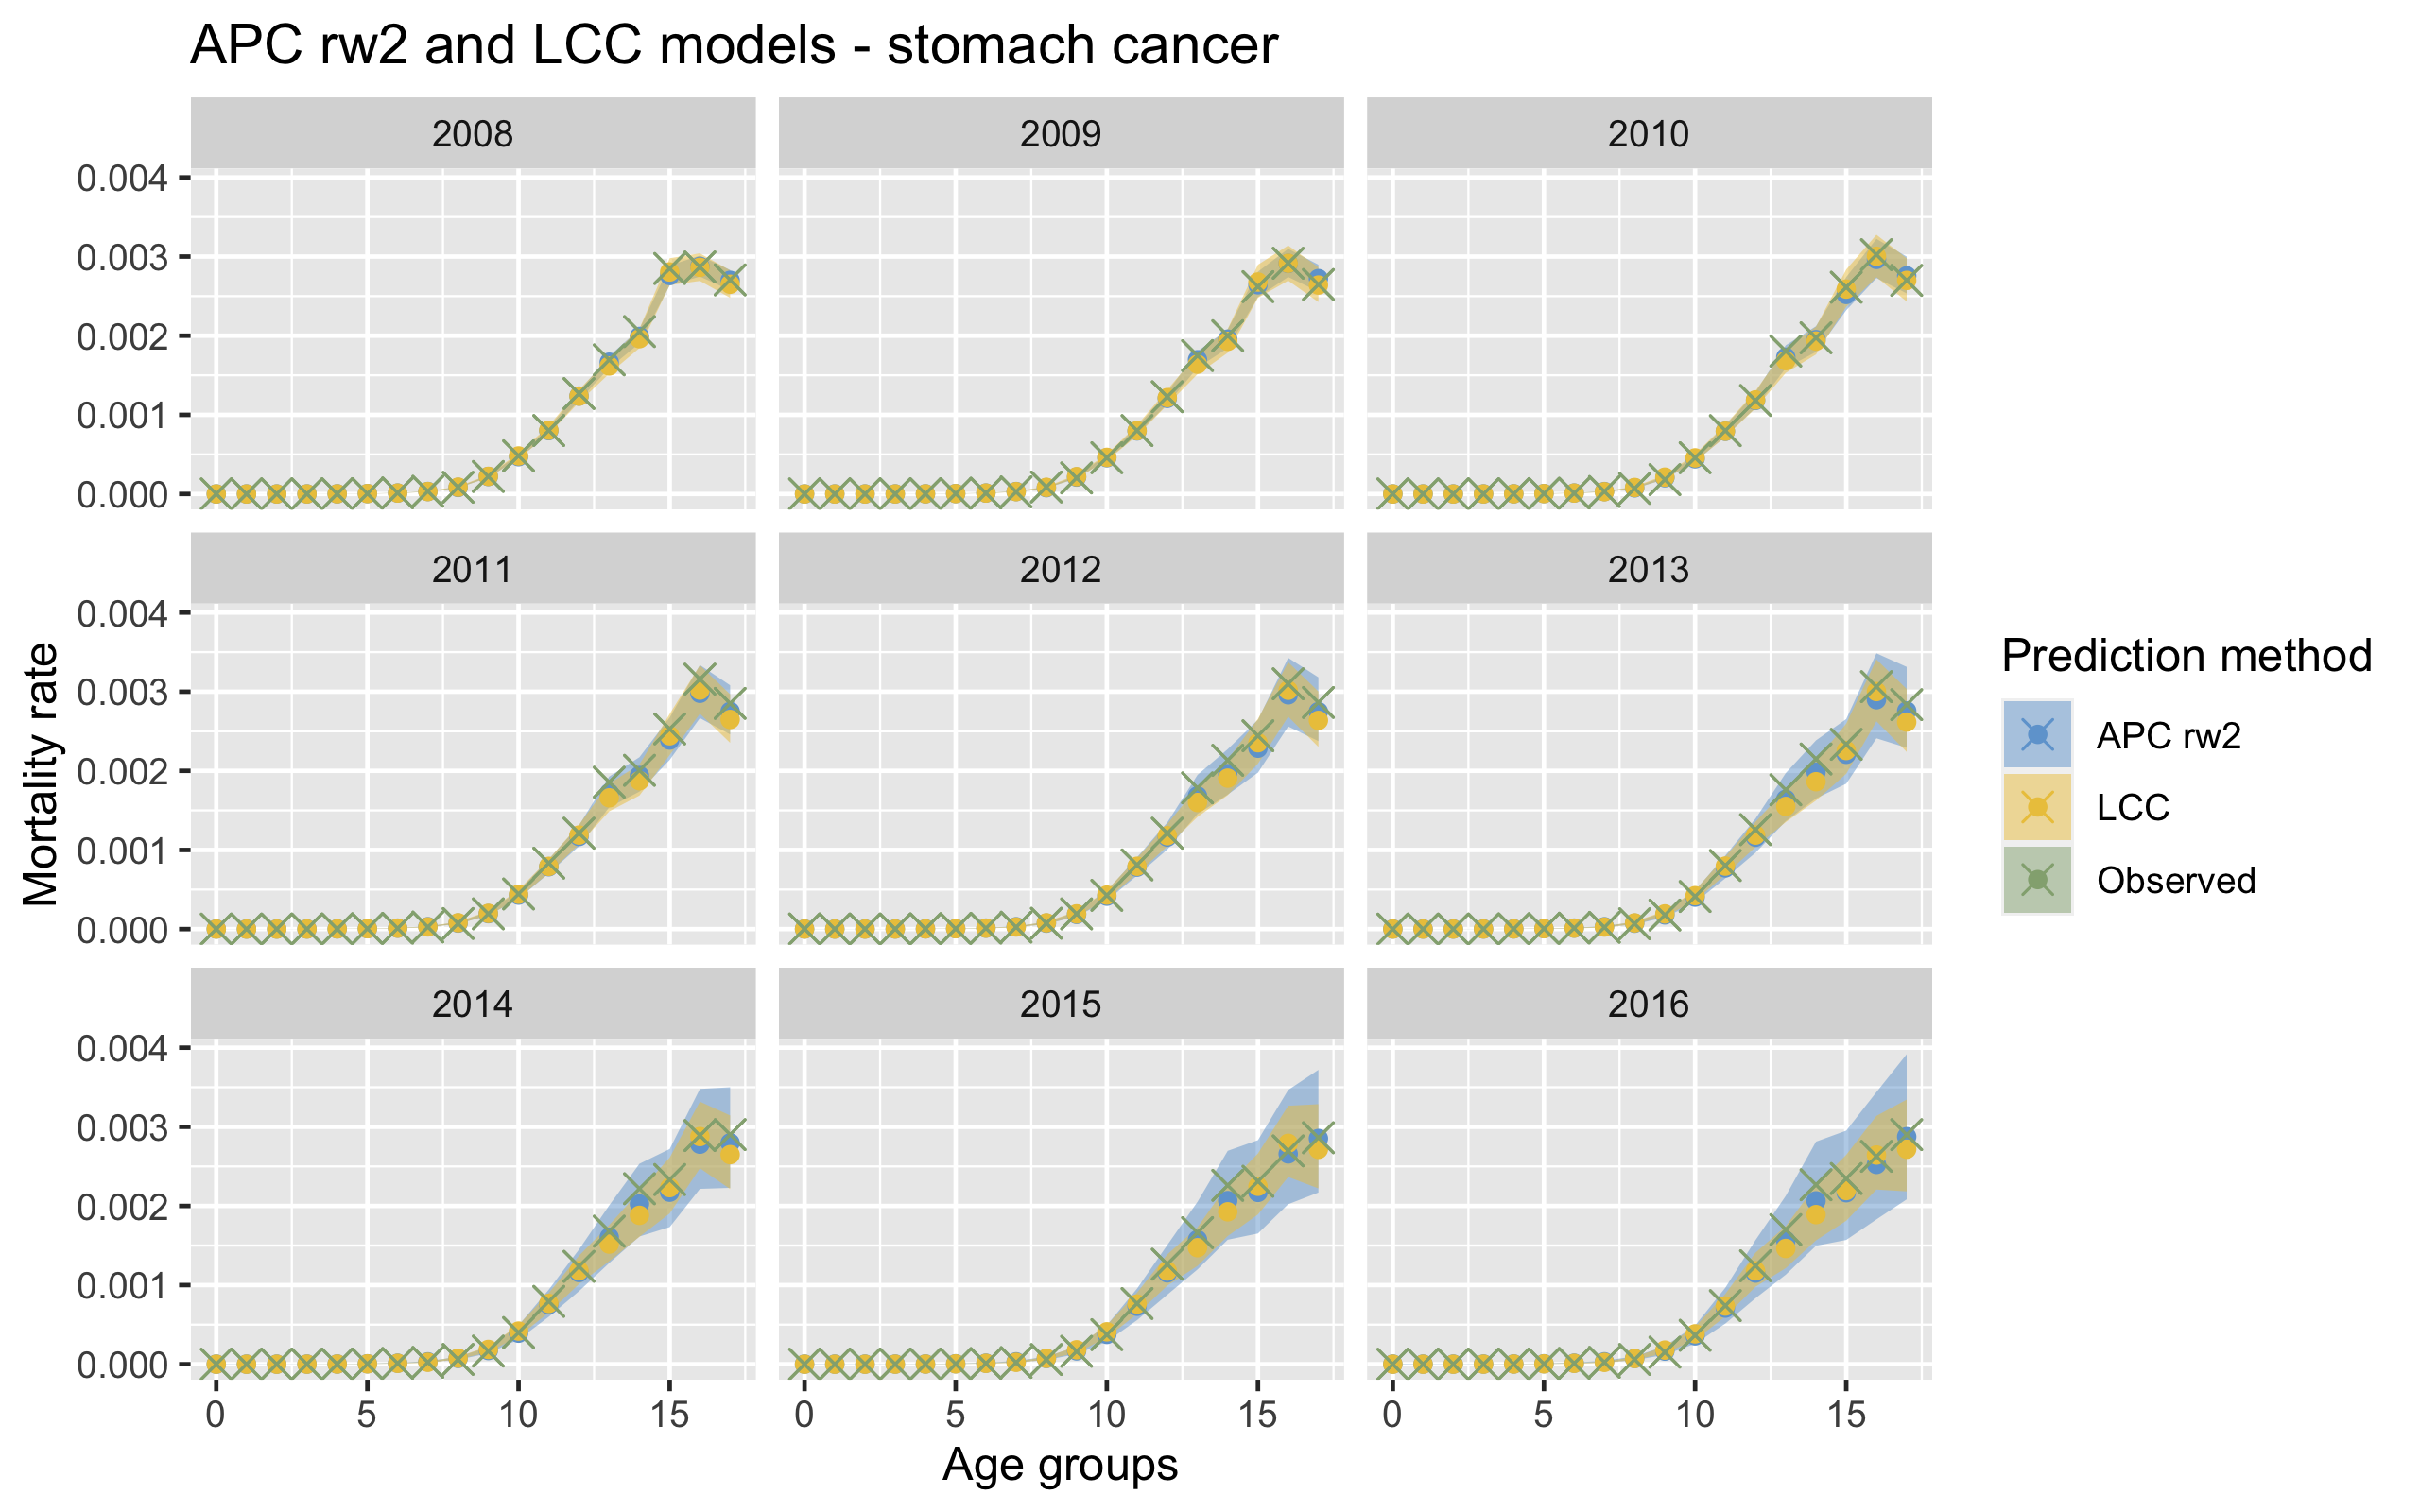
\includegraphics[width=\linewidth]{real-data/real-data-univariate/Figures/univariate-comparison-by-age-lung.png}
    \end{subfigure}
    \begin{subfigure}[b]{.45\linewidth}
        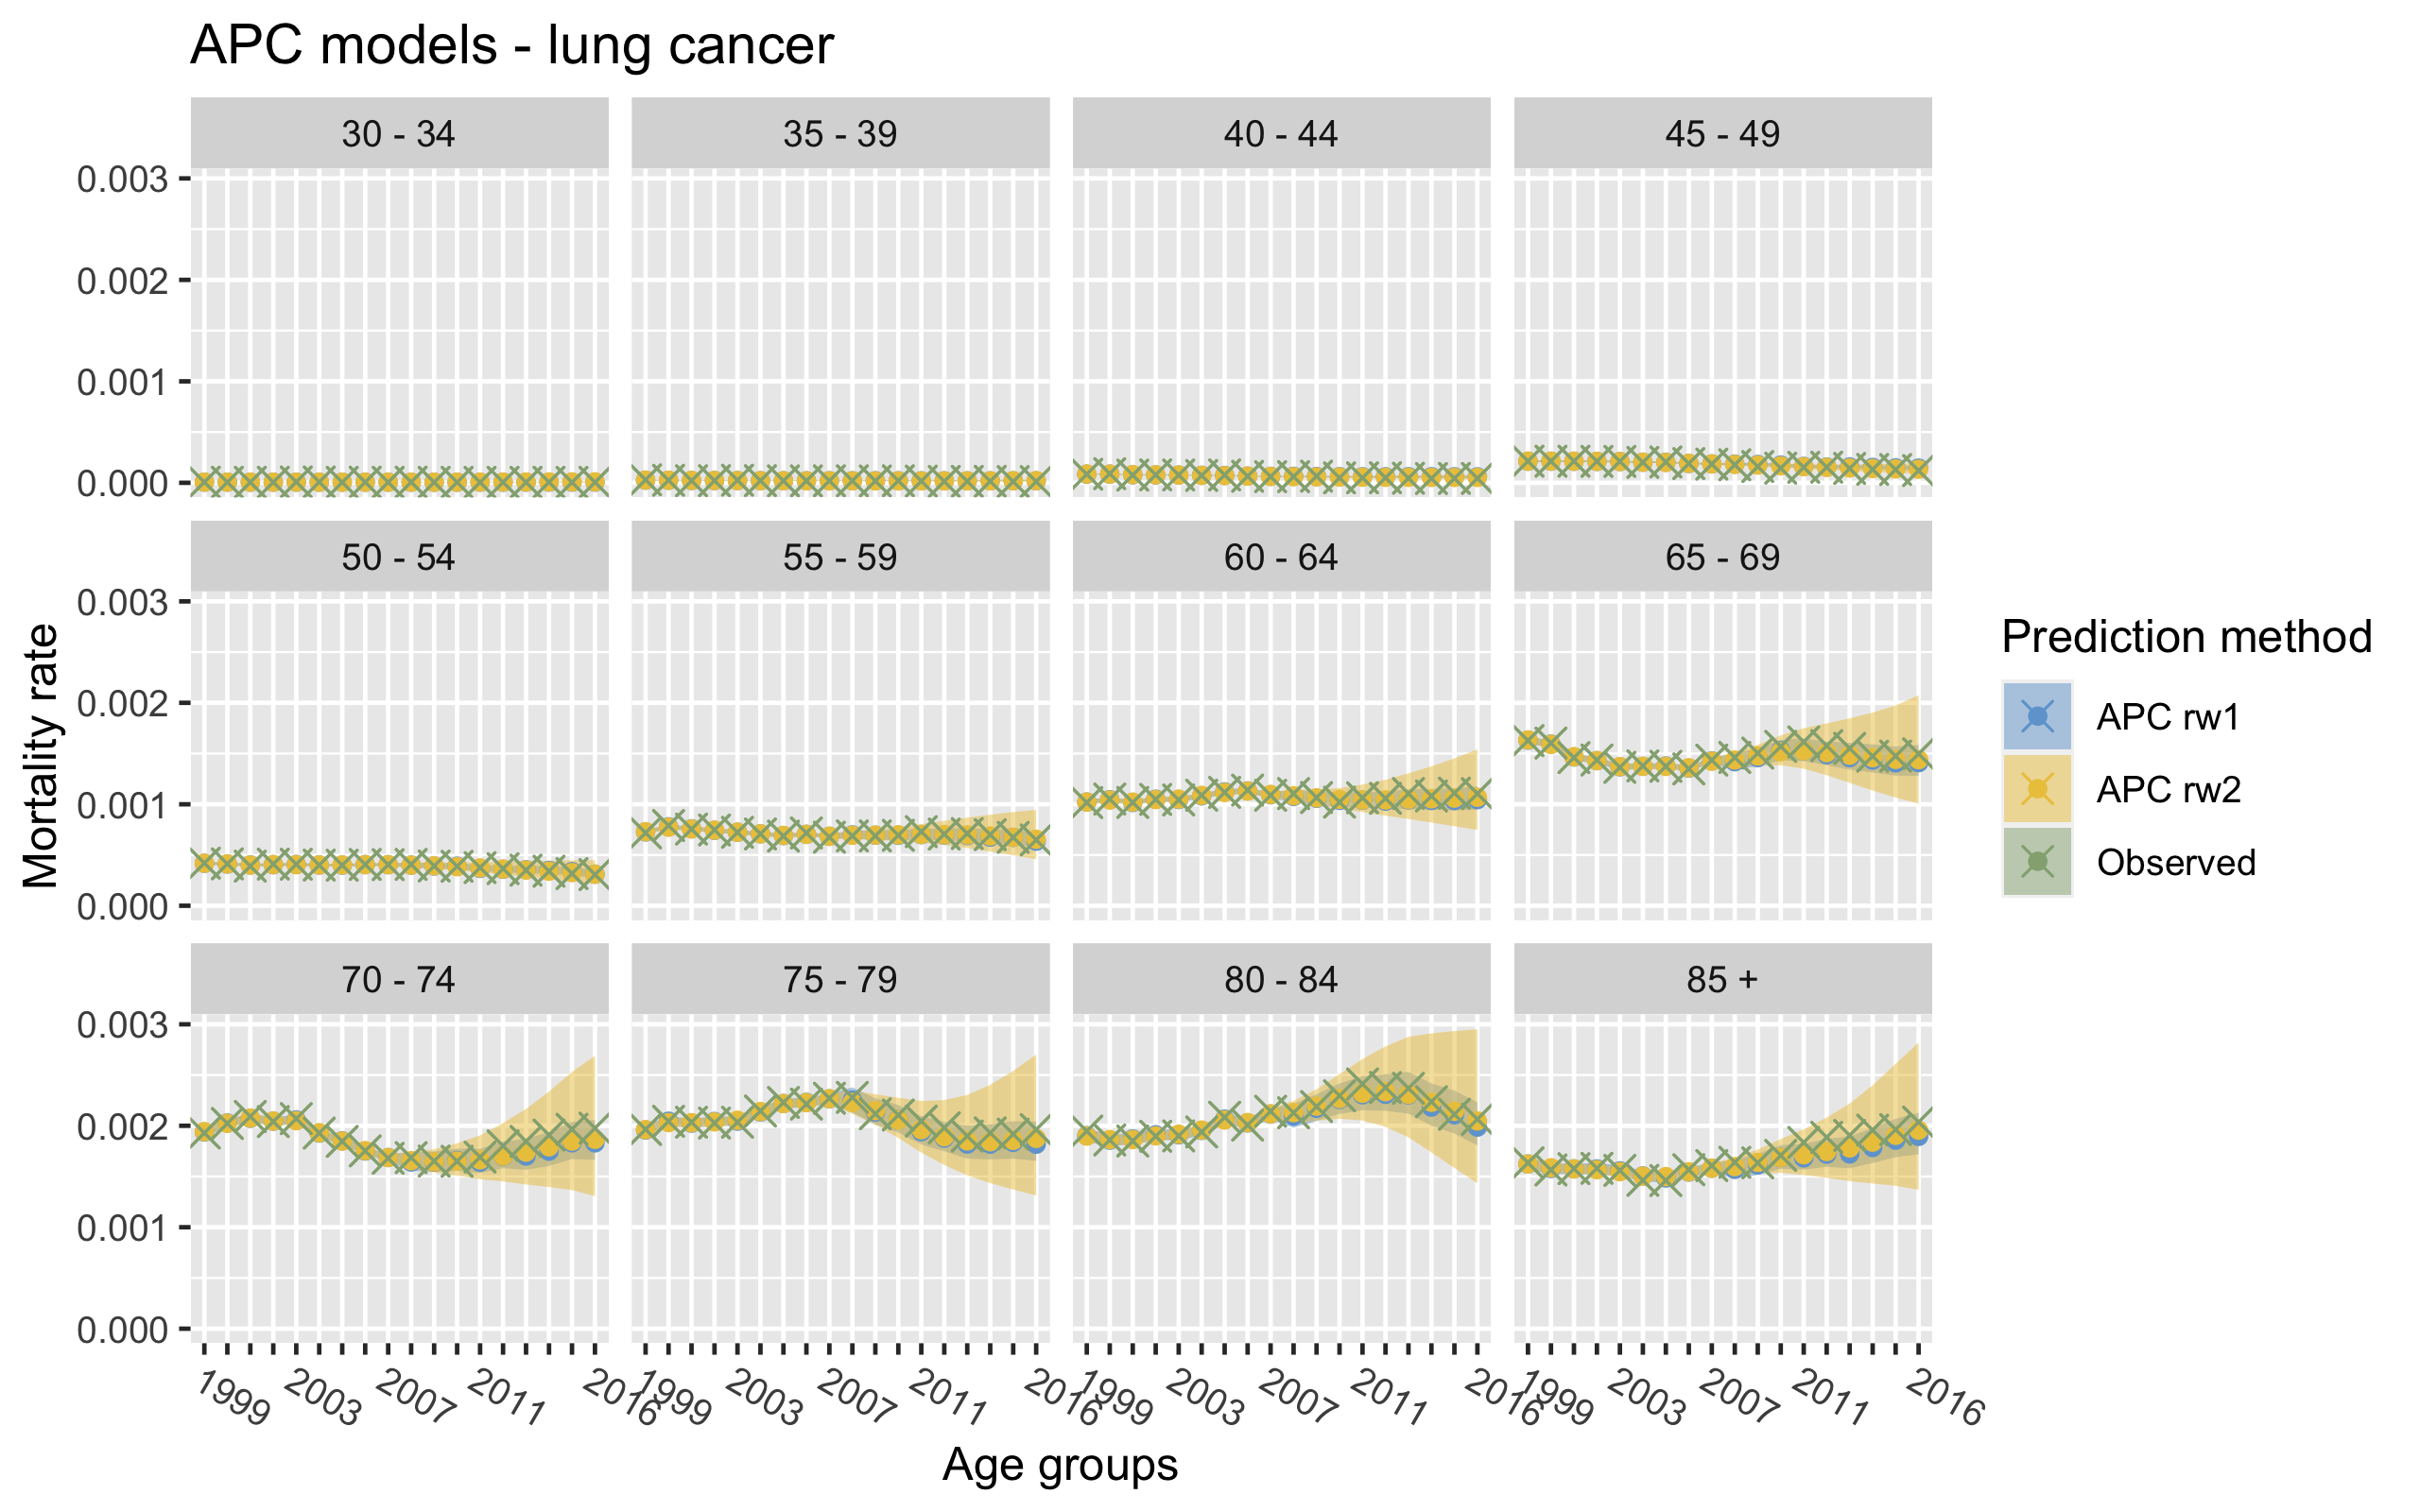
\includegraphics[width=\linewidth]{real-data/real-data-univariate/Figures/univariate-comparison-by-period-lung.png}
    \end{subfigure}
    \caption{The best-performing APC and LC-type models for lung cancer}
    \label{fig:uv-comparison-lung}
\end{figure}

\begin{figure}[h!]
    \centering
    \begin{subfigure}[b]{.45\linewidth}
        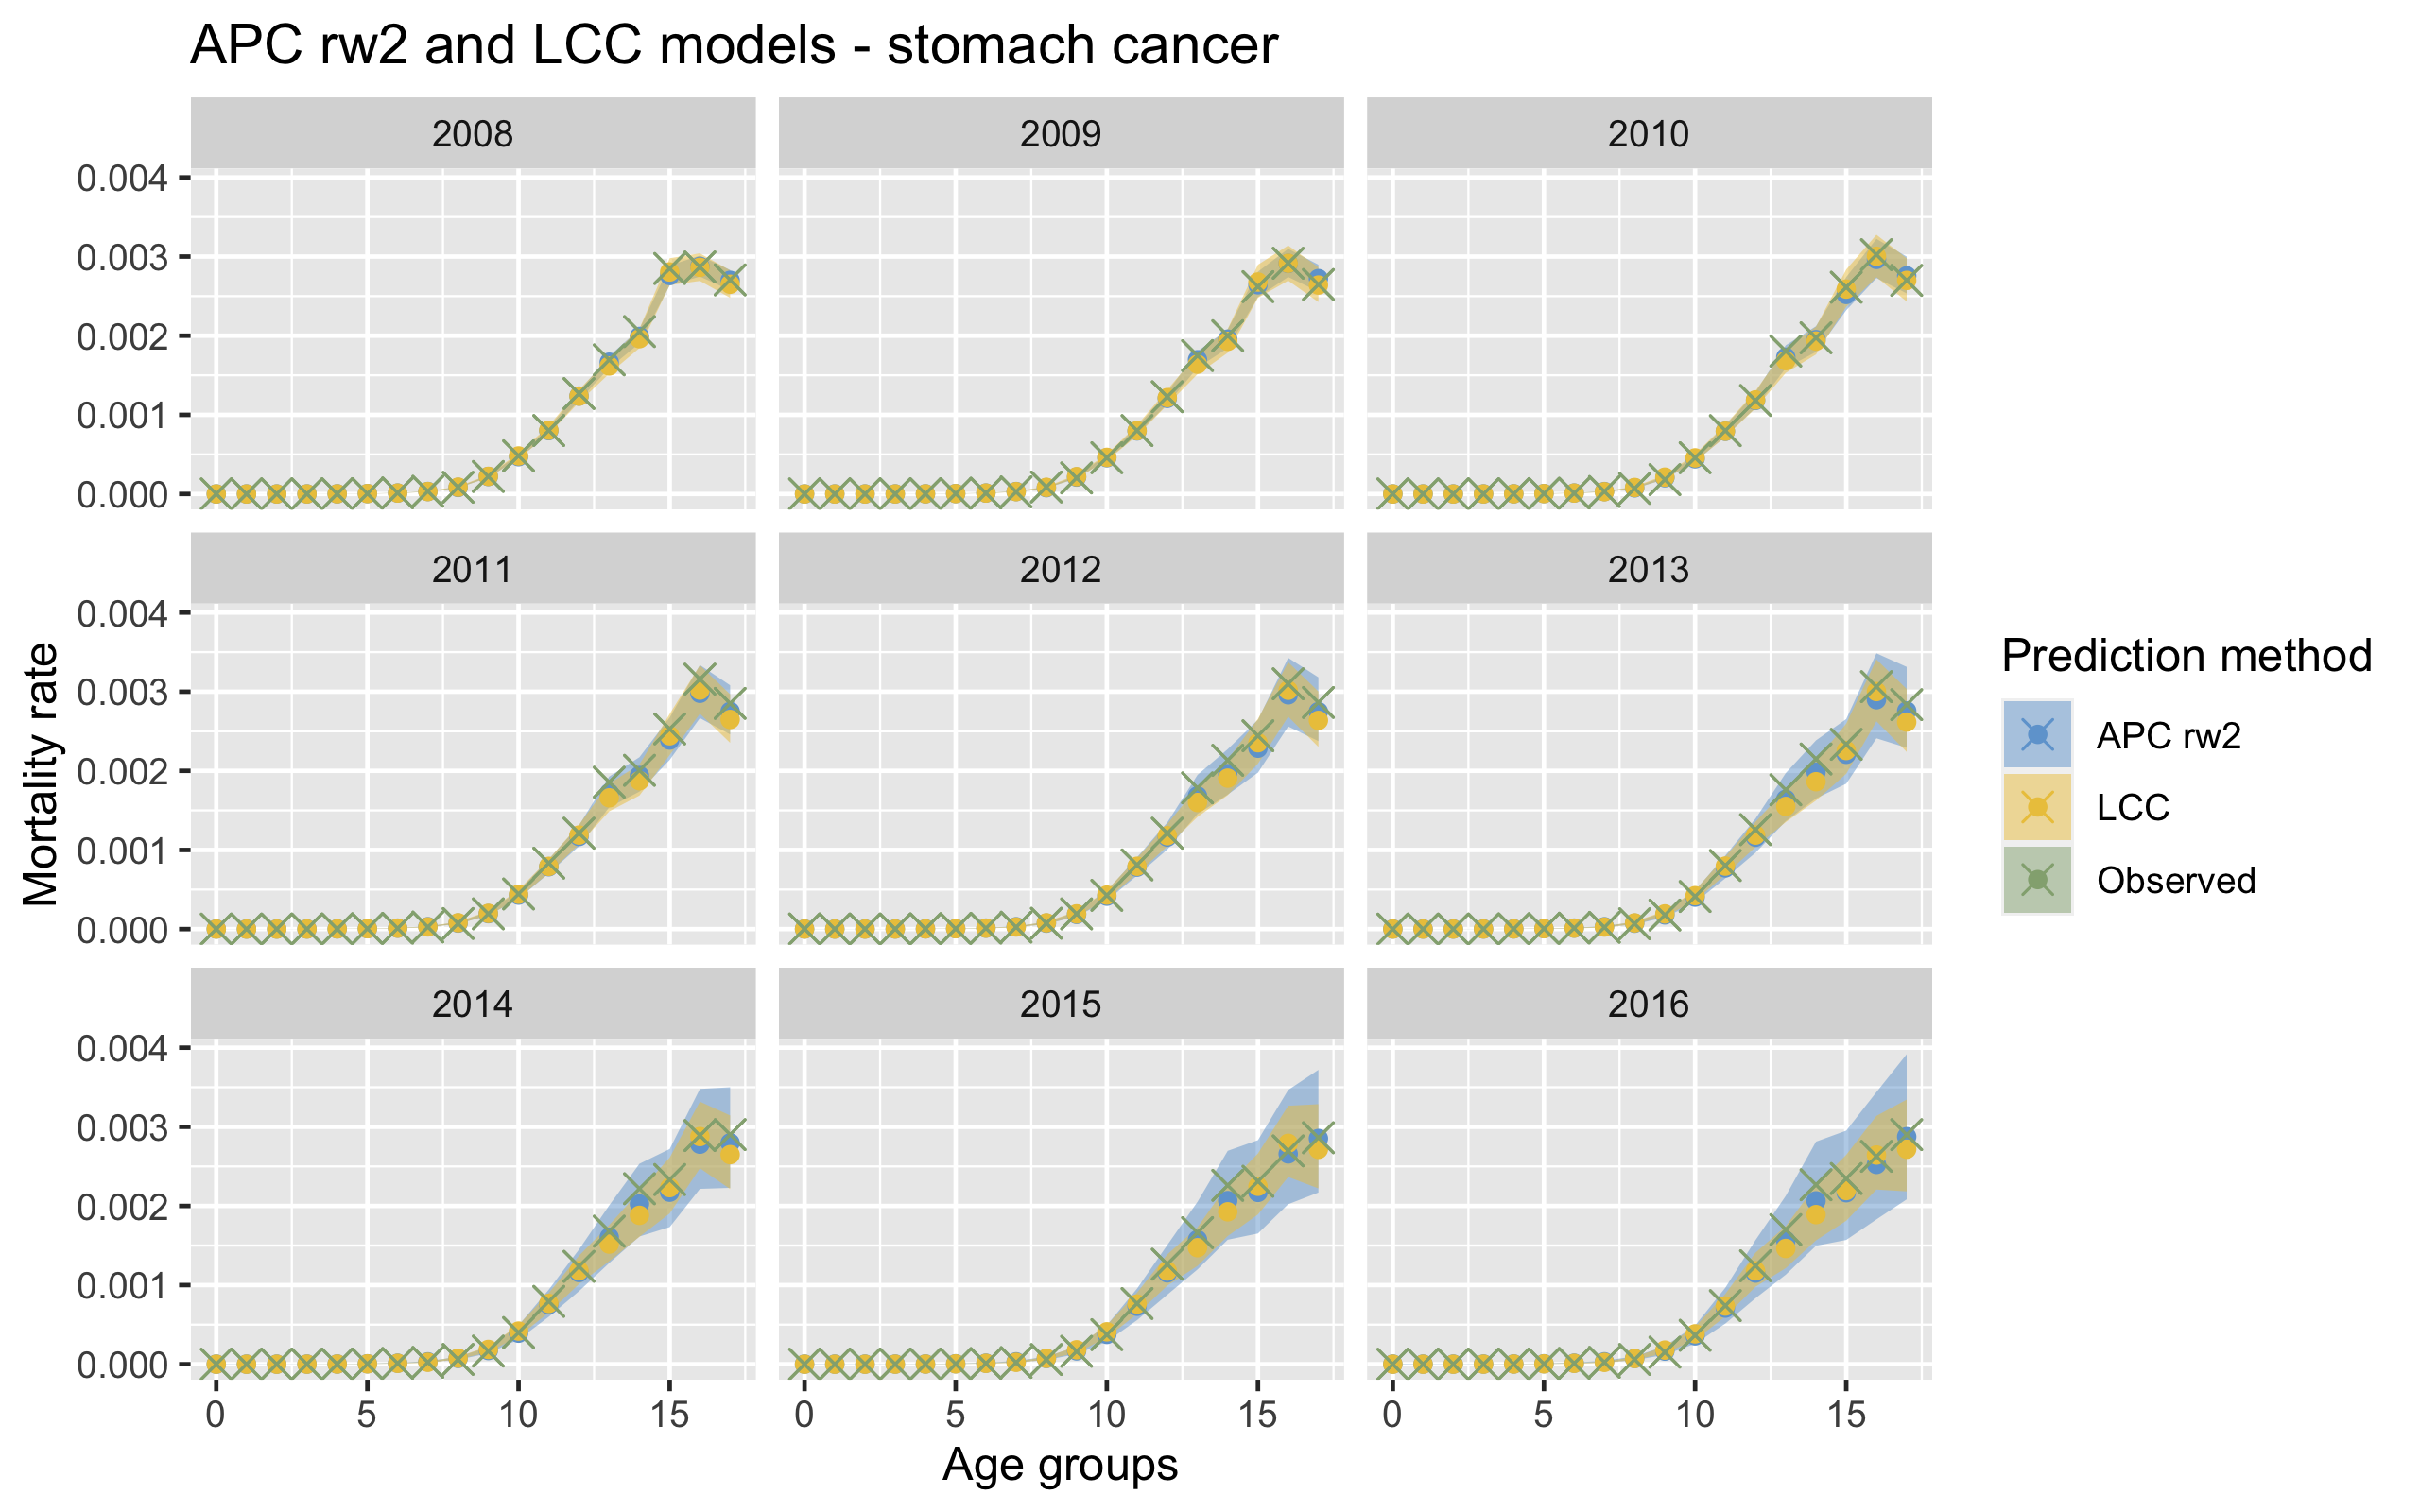
\includegraphics[width=\linewidth]{real-data/real-data-univariate/Figures/univariate-comparison-by-age-stomach.png}
    \end{subfigure}
    \begin{subfigure}[b]{.45\linewidth}
        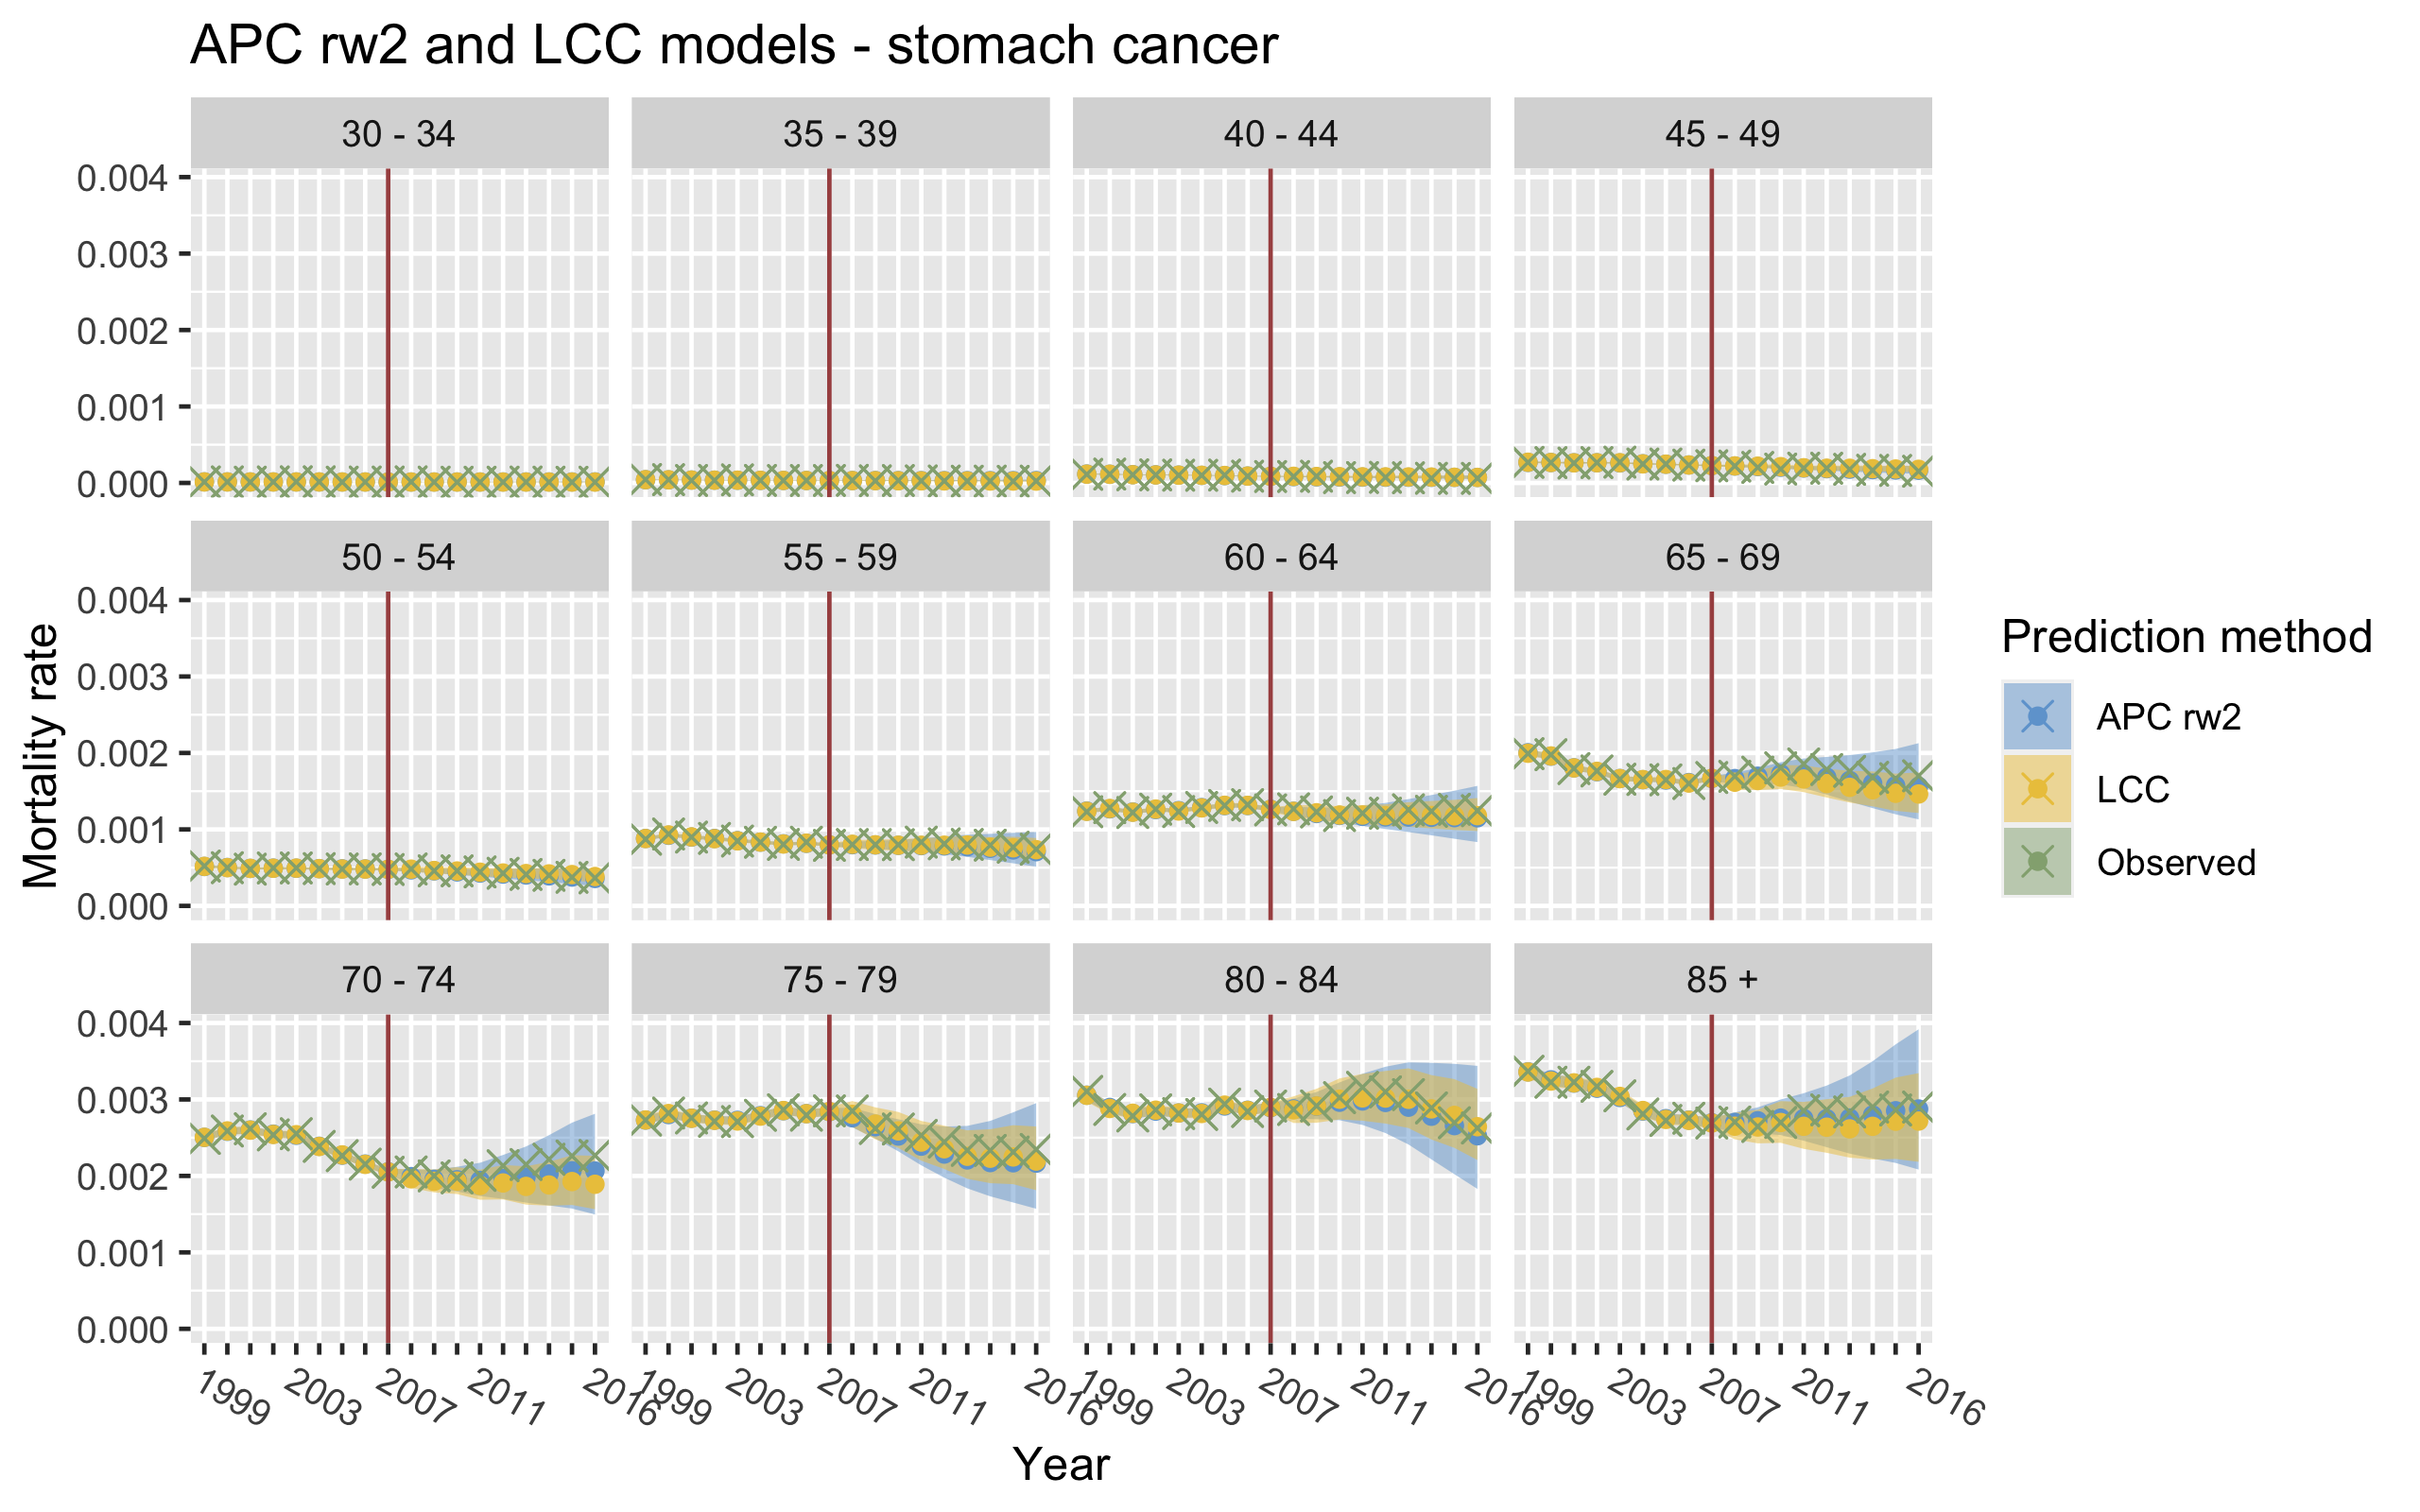
\includegraphics[width=\linewidth]{real-data/real-data-univariate/Figures/univariate-comparison-by-period-stomach.png}
    \end{subfigure}
    \caption{The best-performing APC and LC-type models for stomach cancer}
    \label{fig:uv-comparison-stomach}
\end{figure}

Figures \ref{fig:uv-comparison-lung} and \ref{fig:uv-comparison-stomach} display the results from the Lee-Carter and the APC models with the lowest MDSS, the LCC- and the APC2-models respectively. For both cancer types, the APC2 model has the lowest MDSS, and we see from the plotted results that it seem to be slightly more accurate than the LCC model. We do, however note that the prediction intervals are narrower for the LCC model predictions for both cancer types. \textcolor{myDarkGreen}{Say anything more about this? }

\newpage
\subsection{Prediction in the Multivariate Case}

\textcolor{myDarkGreen}{
Intro: forskjell på multivariate og univariate. Referer til figuren av plottet data - tydelig forskjell på kjønnene, som kan tyde på at en multivariate modell vil fungere bedre. 
\newline \newline 
Hvilke modeller tester du? Her bør du ha snakket om tidligere hvilke modeller som kunne ha blitt testet (common age, period cohort og alle kombinasjonene) på et generelt nivå, og her forteller du hvordan disse appliseres (?) til de to beste modellene fra univariate analyse (LCC og APC2). Skriv opp disse modellene eksplisitt, og forklar notasjonen din. 
\newline \newline
Fortell hva slags priors du har brukt, og fortell om hvordan du implementerer multivariate modeller i inlabru. Ha kanskje med en kodesnutt for å vise syntaksen. 
}

\textcolor{myDarkGreen}{Thought: For the multivariate version where all effects are kept common, you should also have a common intercept! If not it might be very different to adjust one random effect to two different overall mortality rates?}

From the plots of the cancer mortality data in Section \ref{sec:GermanCancerData}, we observe a significant difference in male and female mortality rates, for both cancer types. The investigation of multivariate models with sex as a covariate, is then a natural next step in our analysis. We fit different multivariate models, as outlined in Section \ref{sec:multivariateAPC}, and compare the results. In other words, we now fit multivariate versions of Lee-Carter and APC models to the observed male and female cancer deaths, and use the male and female populations as the at-risk values. To avoid having to compare too many different models, we test only the Lee-Carter and APC models that displayed the best MDSS in the univariate case, namely the LCC-model and the APC2-model (for both lung and stomach cancer). It is not clear from the plots of the data which, if any, of the effects that should be kept common for male and female populations. Therefore, we find predictions using models with all combinations of common and separate age, period and cohort effects, and compare the results. We test the following versions of the LCC-model:
\begin{itemize}
    \item All common: $\eta_{x,t,s} = \mu_s + \alpha_x + \beta_x(\phi\cdot t + \kappa_t) + \gamma_k + \epsilon_{x,t,s}$
    \item Common age, period: $\eta_{x,t,s} = \mu_s + \alpha_x + \beta_x(\phi\cdot t + \kappa_t) + \gamma_{k,s} + \epsilon_{x,t,s}$
    \item Common age, cohort: $\eta_{x,t,s} = \mu_s + \alpha_x + \beta_x(\phi_s\cdot t + \kappa_{t,s}) + \gamma_{k} + \epsilon_{x,t,s}$
    \item Common period, cohort: $\eta_{x,t,s} = \mu_s + \alpha_{x,s} + \beta_{x,s}(\phi\cdot t + \kappa_t) + \gamma_{k} + \epsilon_{x,t,s}$
    \item Common age: $\eta_{x,t,s} = \mu_s + \alpha_x + \beta_x(\phi_s\cdot t + \kappa_{t,s}) + \gamma_{k,s} + \epsilon_{x,t,s}$
    \item Common period: $\eta_{x,t,s} = \mu_s + \alpha_{x,s} + \beta_{x,s}(\phi\cdot t + \kappa_{t}) + \gamma_{k,s} + \epsilon_{x,t,s}$
    \item Common cohort: $\eta_{x,t,s} = \mu_s + \alpha_{x,s} + \beta_{x,s}(\phi_s\cdot t + \kappa_{t,s}) + \gamma_{k} + \epsilon_{x,t,s}$
    \item No common: $\eta_{x,t,s} = \mu_s + \alpha_{x,s} + \beta_{x,s}(\phi_s\cdot t + \kappa_{t,s}) + \gamma_{k,s} + \epsilon_{x,t,s}$
\end{itemize}
Note that the "No common" version of the model is equivalent to fitting two separate univariate LCC models to the male and female parts of the data. Note also that we always keep $\alpha_x$ and $\beta_x$ either common or separate, we could have also included all versions of the model where one is kept common and the other is separate. We do not do this, simply to reduce the number of models we need to compare, and because we do not expect it to have a lot of impact on the result. \textcolor{myDarkGreen}{Do you have enough reason to say this? }
For the APC2-model, we test the following multivariate versions:
\begin{itemize}
    \item APC: $\eta_{x,t,s}= \mu_{s} + \rho_x + \phi_t + \psi_k + \epsilon_{x,t,s}$ 
    \item APc: $\eta_{x,t,s}= \mu_{s} + \rho_x + \phi_t + \psi_{k,s} + \epsilon_{x,t,s}$ 
    \item ApC: $\eta_{x,t,s}= \mu_{s} + \rho_x + \phi_{t,s} + \psi_{k} + \epsilon_{x,t,s}$ 
    \item aPC: $\eta_{x,t,s}= \mu_{s} + \rho_{x,s} + \phi_{t} + \psi_{k} + \epsilon_{x,t,s}$ 
    \item aPc: $\eta_{x,t,s}= \mu_{s} + \rho_{x,s} + \phi_{t} + \psi_{k,s} + \epsilon_{x,t,s}$ 
    \item apC: $\eta_{x,t,s}= \mu_{s} + \rho_{x,s} + \phi_{t, s} + \psi_{k} + \epsilon_{x,t,s}$ 
    \item apc: $\eta_{x,t,s}= \mu_{s} + \rho_{x,s} + \phi_{t, s} + \psi_{k, s} + \epsilon_{x,t,s}$
\end{itemize}
Following \textcite{rieblerHeld2010}, we name the different versions of the APC2-model by capital letter for the common effects and shared letters for the male- and female-specific effects. We present the results for lung and stomach cancer, respectively, in the following two sections. 
\newpar We alter the implementation of the prediction in \inlabru compared to the implementation of the univariate models. To implement the multivariate models, we use two likelihoods, one for each sex. For the effects that will not be common for male and females, we include two identical model components, named differently. These are included in one likelihood each. For the effects that are kept common, we only include one model component, which is used in both likelihoods. We only include male data in the male likelihood and female data in the female likelihood. Below, the part of the code used to produce predictions for the aPc-model is shown:


\subsubsection{Lung cancer data}
\textcolor{myDarkGreen}{
Inkluder først og fremst resultatene, og kommebter kort hva de viser. Her bør du også diskutere hvordan noen av konfigurasjonene ikke konvergerte for LCC modellene - finn en god måte å skrive det inn i resultatene. Fortell hvor mange iterasjoner du satte som maks. Snakk om at det er "reasonable to assume" at dette ikke gir noen forskjell på resultatet. Det at modellen bruker lang tid på å konveregere er i seg selv et tegn på at modellen ikke er godt egnet til å tilpasse dataen (?), i tillegg ser vi fra APC resultatene at modeller med mange felles effekter gir tydelig dårligere prediksjoner enn modeller med få felles effekter. Det er dermed ingen grunn til å tro at modellene som ikke konvergerte ville ha gitt bedre prediksjoner. 
Figurer:
\begin{itemize}
    \item Score for LCC-modeller (tabell)
    \item Score for APC-modeller (tabell)
    \item plott av to beste LCC
    \item plott av to beste APC
    \item Plott av beste APC sammen med beste LCC
    \item Plott av LCC-effekter (for beste modell)
\end{itemize}
}
\begin{table}[h!]
    \begin{tabular}{l |c c c }
        Model & MSE & MDSS & Contained 95\%-interval\\
        \hline
        All common          & 7.318\cdot 10^{-8} & -17.31 (-16.39)    & 0.9630 (0.75) \\
        Common age          & 3.527\cdot 10^{-8} & -18.48 (-19.67)   & 0.7639 (0.6451) \\
        Common age, cohort  & 3.521\cdot 10^{-8} & -16.53 (-19.15)  & 0.7407 (0.6358) \\
        Common age, period  & 4.847\cdot 10^{-8} & -18.31 (-19.06)   & 0.8565 (0.6914) \\
        Common cohort       & 1.705\cdot 10^{-8} & -18.86 (-21.02)  & 0.8519 (0.7222) \\
        Common period       & 2.198\cdot 10^{-8} & \textbf{-19.38} (-20.61)   & 0.9444 (0.7531) \\
        No common           & 2.184\cdot 10^{-8} & \textbf{-19.28} (-21.34)   & 0.9074 (0.7623) \\
    \end{tabular}
    \caption{\label{tab:LCC-lung}Score statistics for the different multivariate LCC models, for the lung cancer data set. The lowest mean DSS values are marked in bold font. }
\end{table}

\begin{figure}[h!]
    \centering
    \begin{subfigure}[b]{.45\linewidth}
        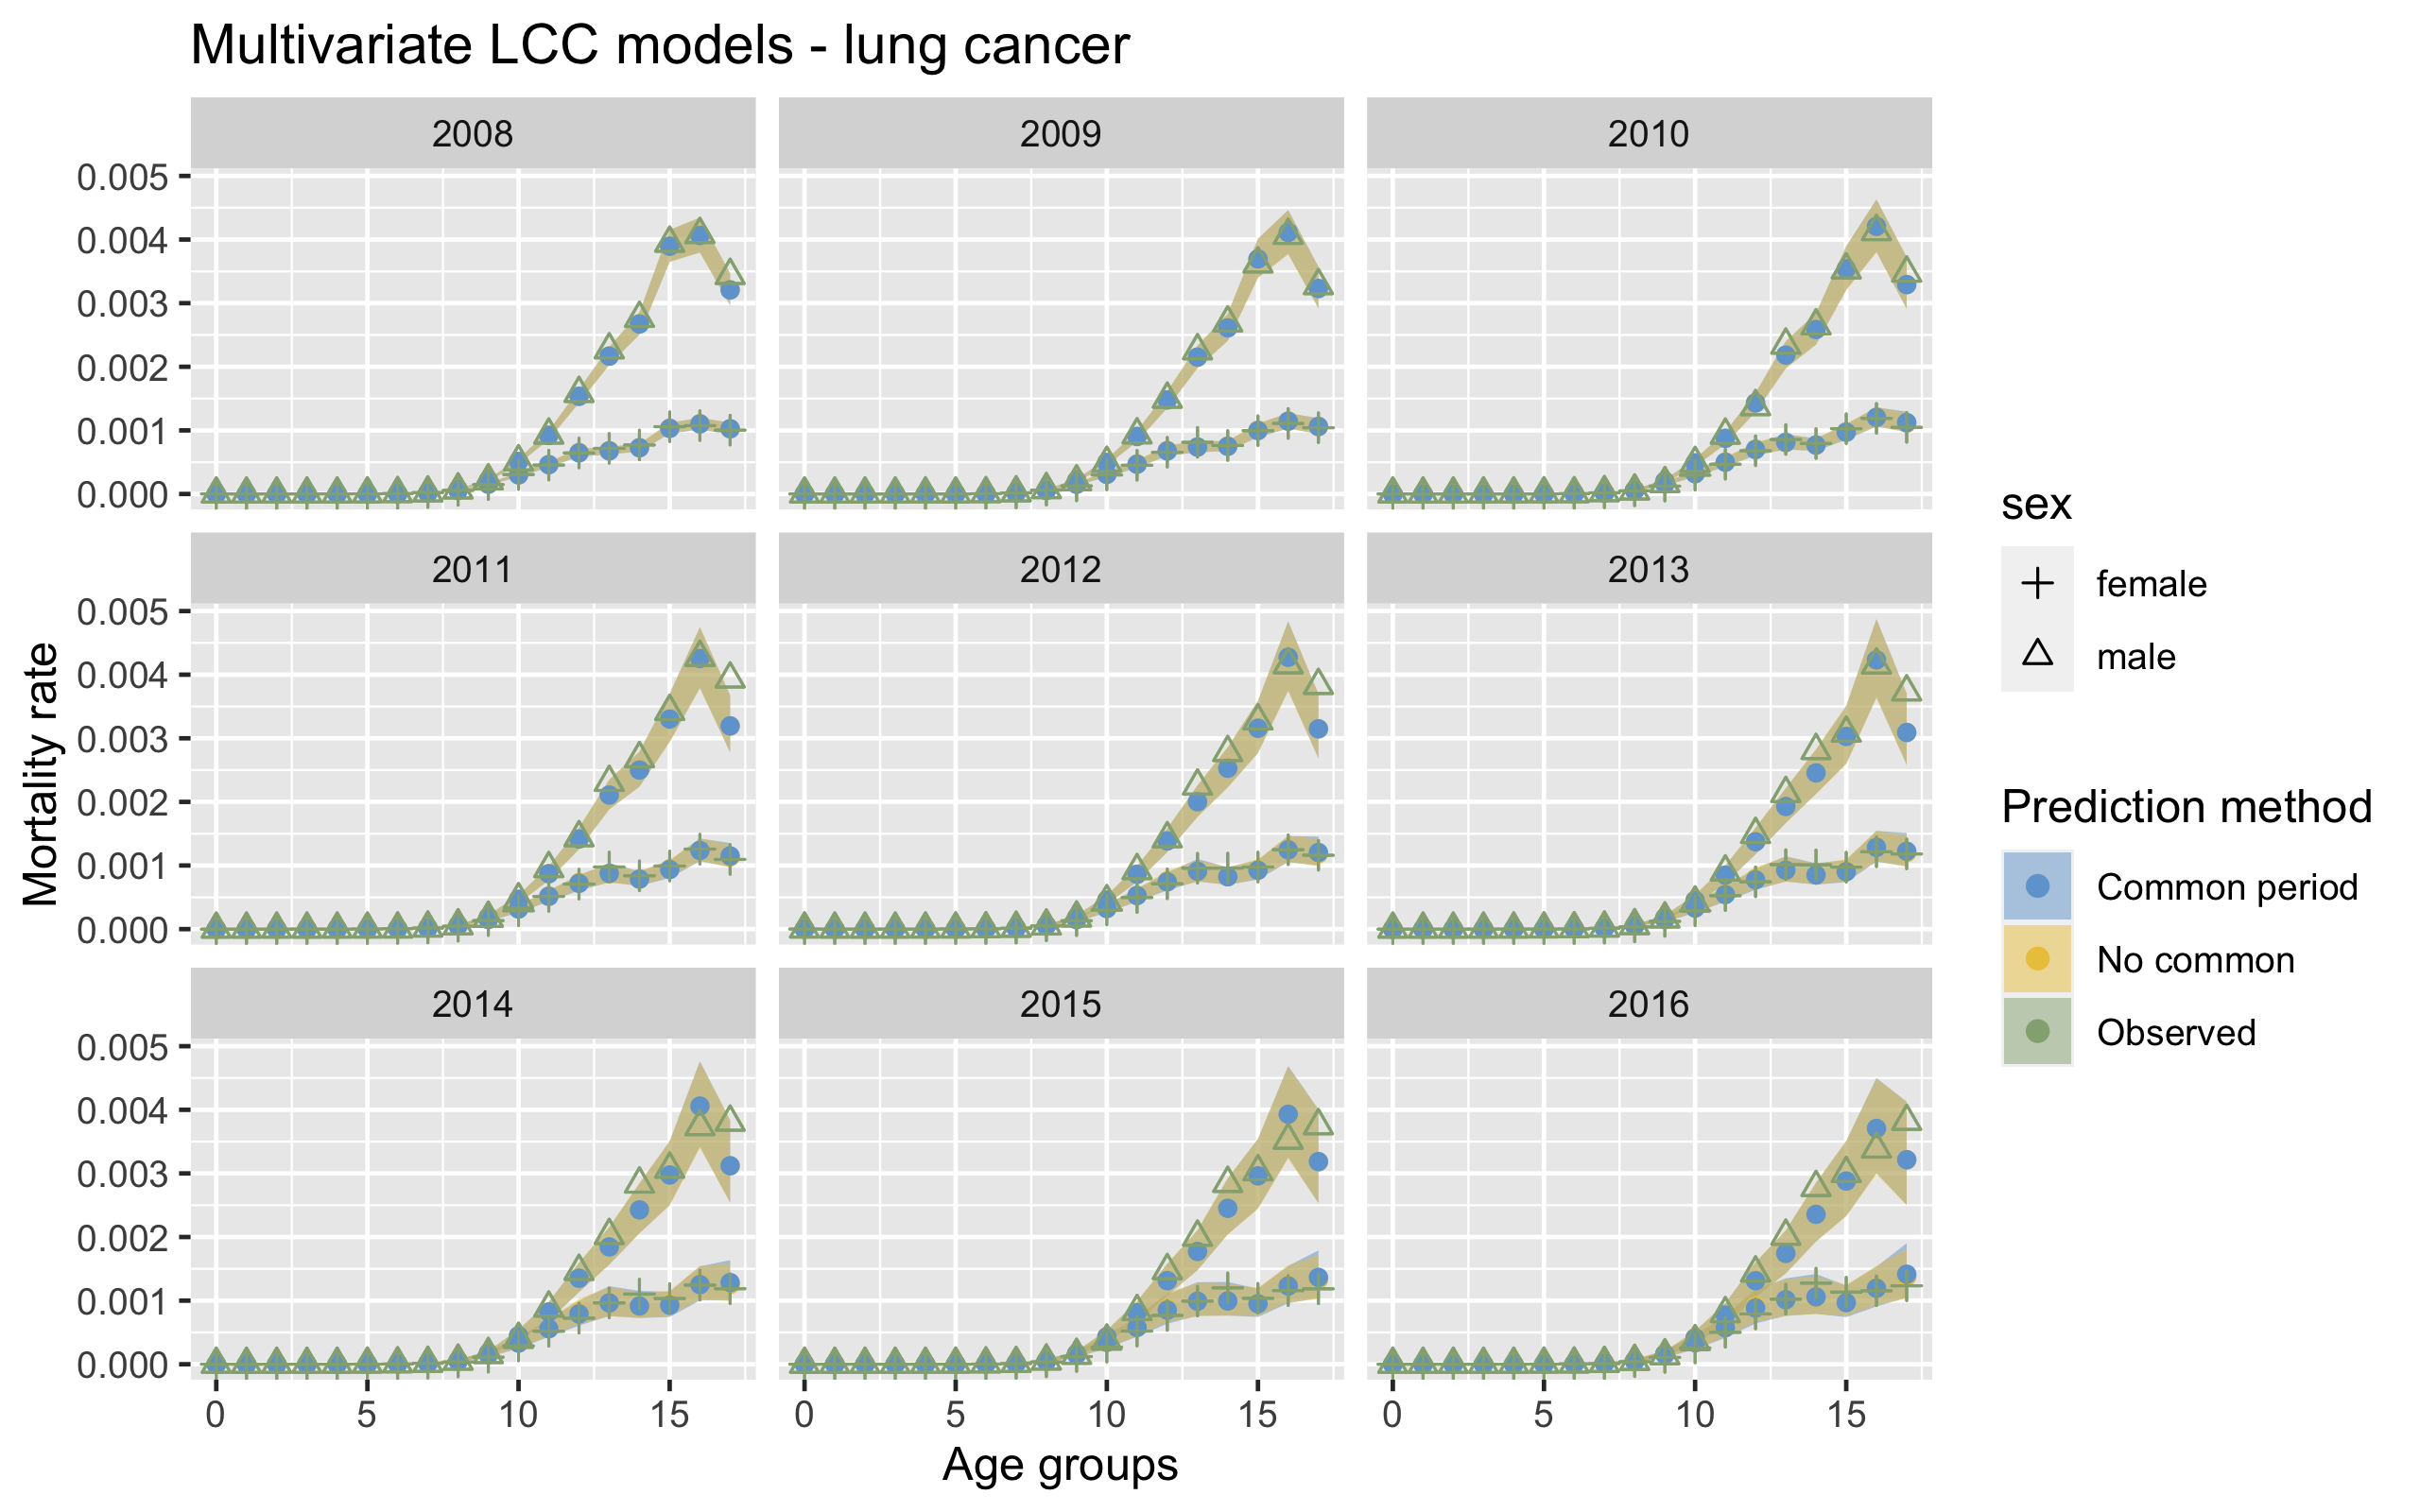
\includegraphics[width=\linewidth]{real-data/real-data-multivariate/Figures/multivariate-LCC-by-age-lung.png}
    \end{subfigure}
    \begin{subfigure}[b]{.45\linewidth}
        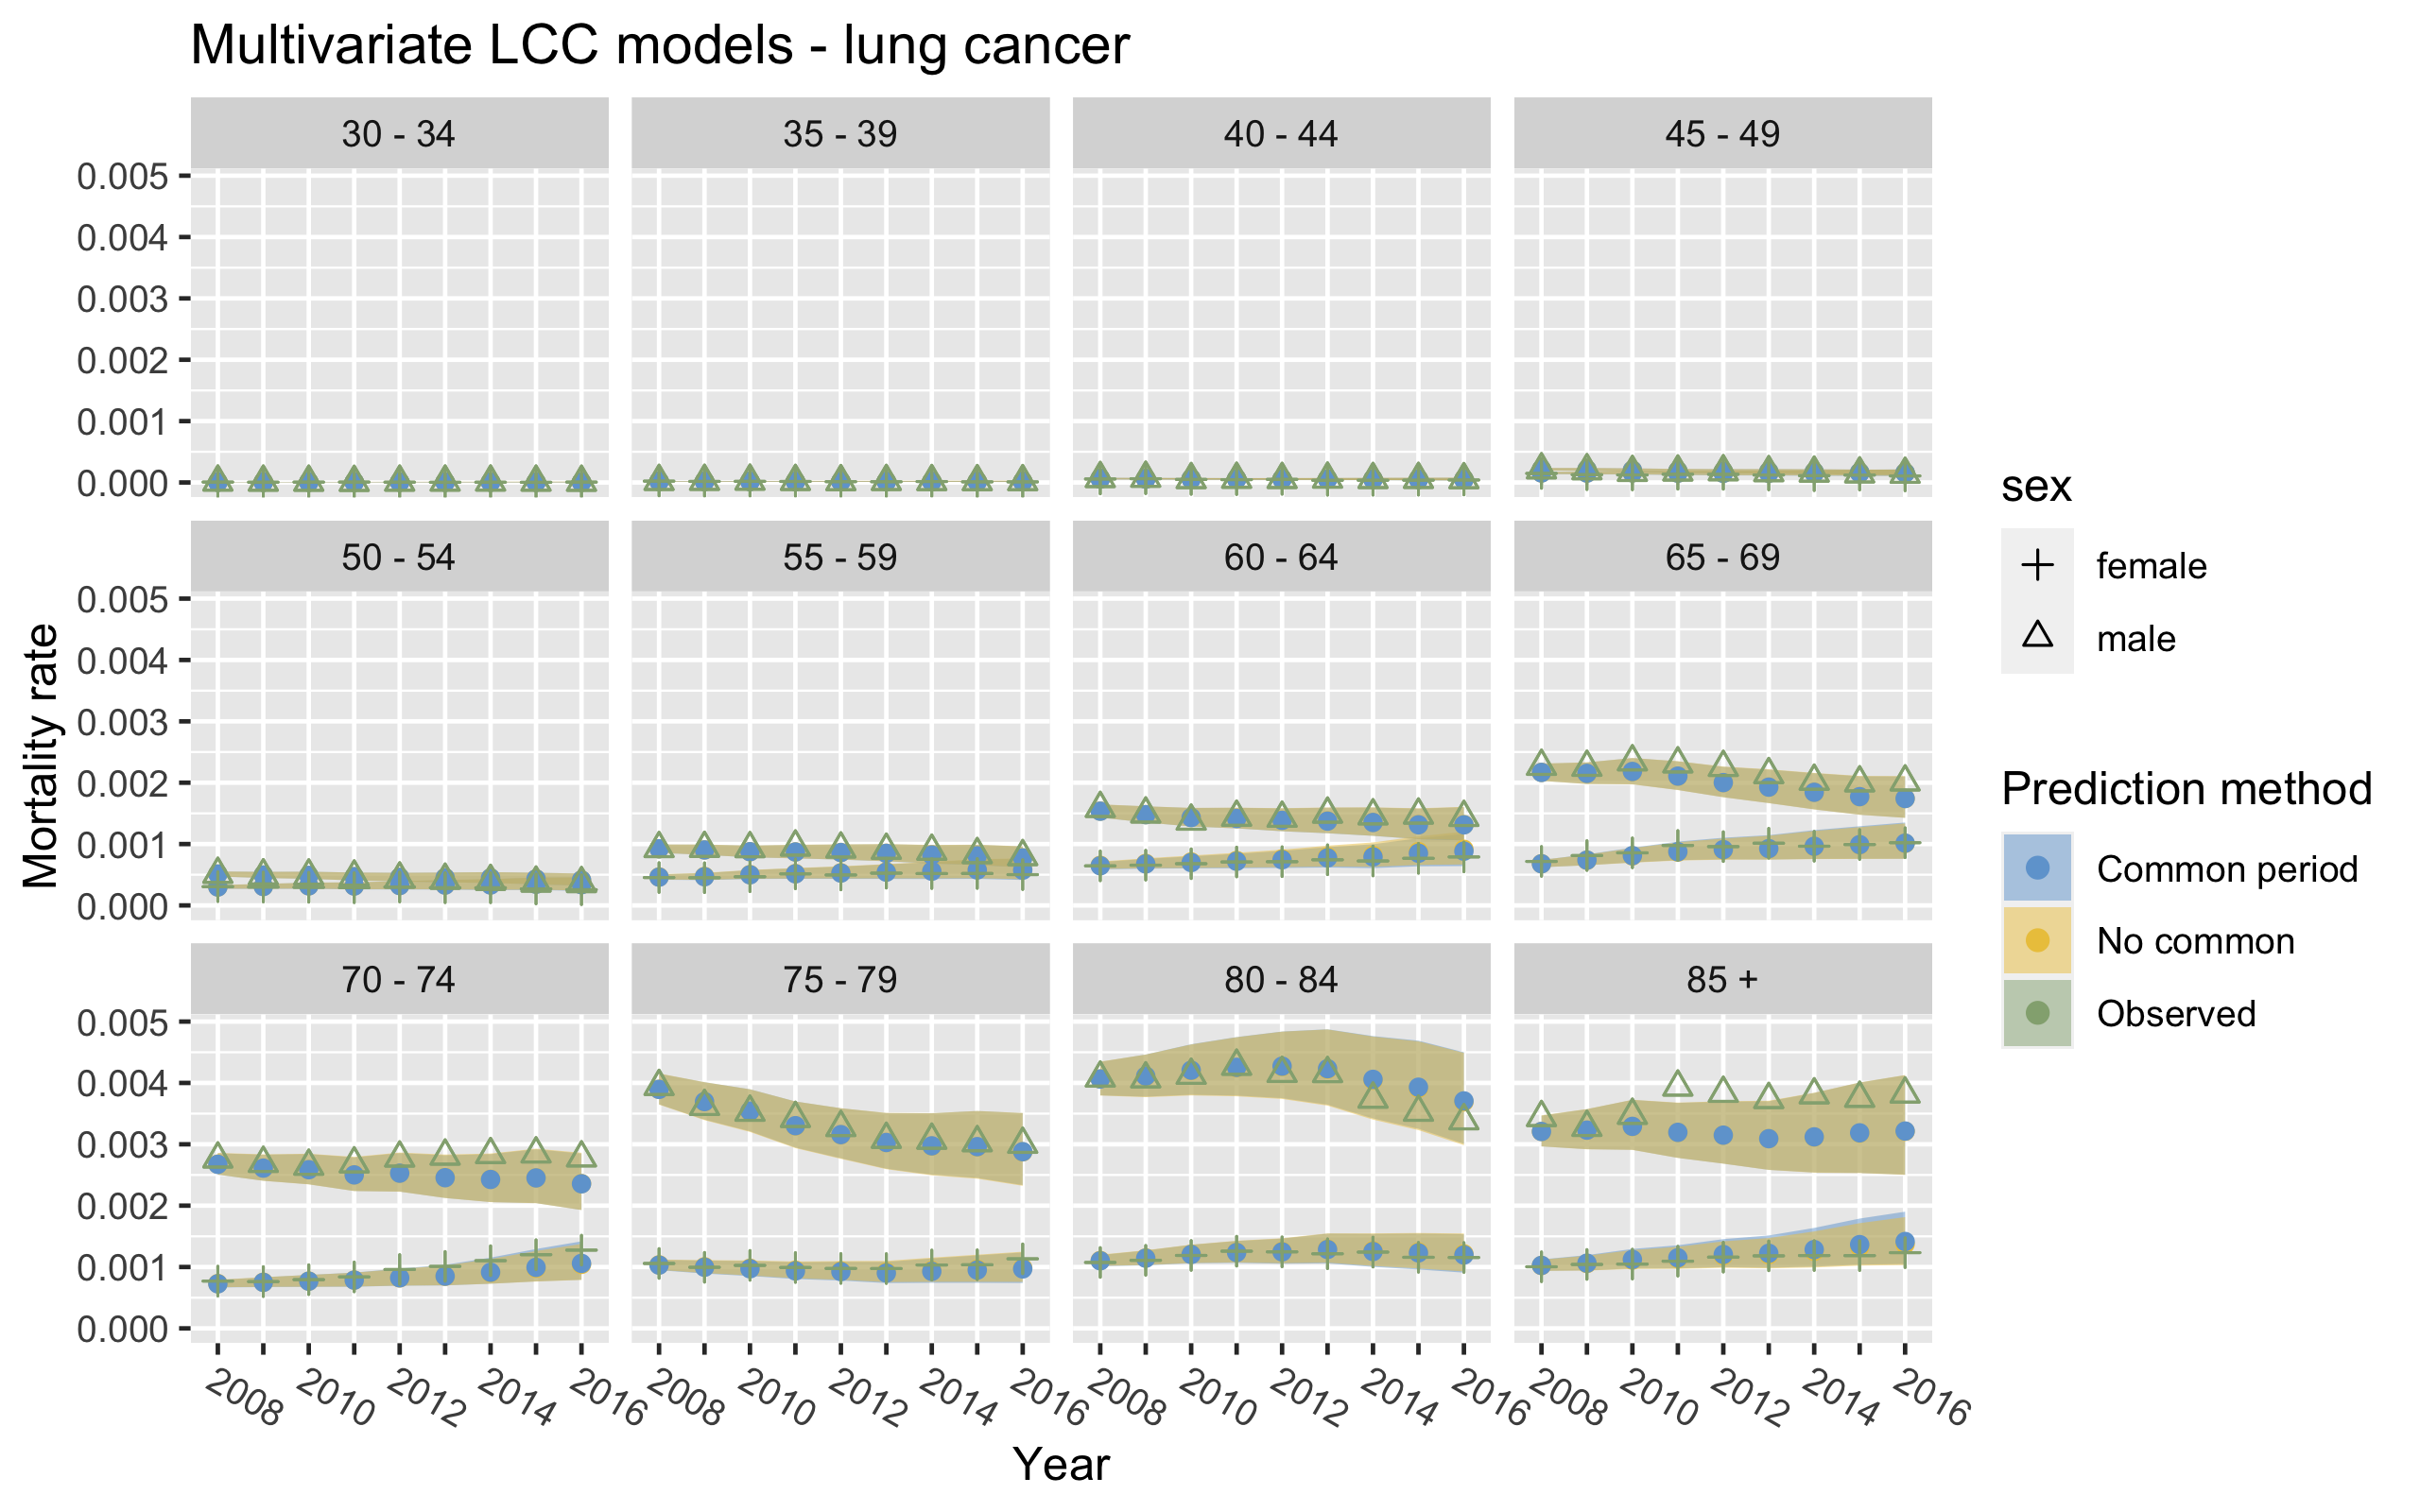
\includegraphics[width=\linewidth]{real-data/real-data-multivariate/Figures/multivariate-LCC-by-period-lung.png}
    \end{subfigure}
    \caption{The two best LCC models - by age (left) and period (right) for the lung cancer data set}
    \label{fig:mv-LCC-lung}
\end{figure}

\begin{figure}[h!]
    \centering
    \begin{subfigure}[b]{.45\linewidth}
        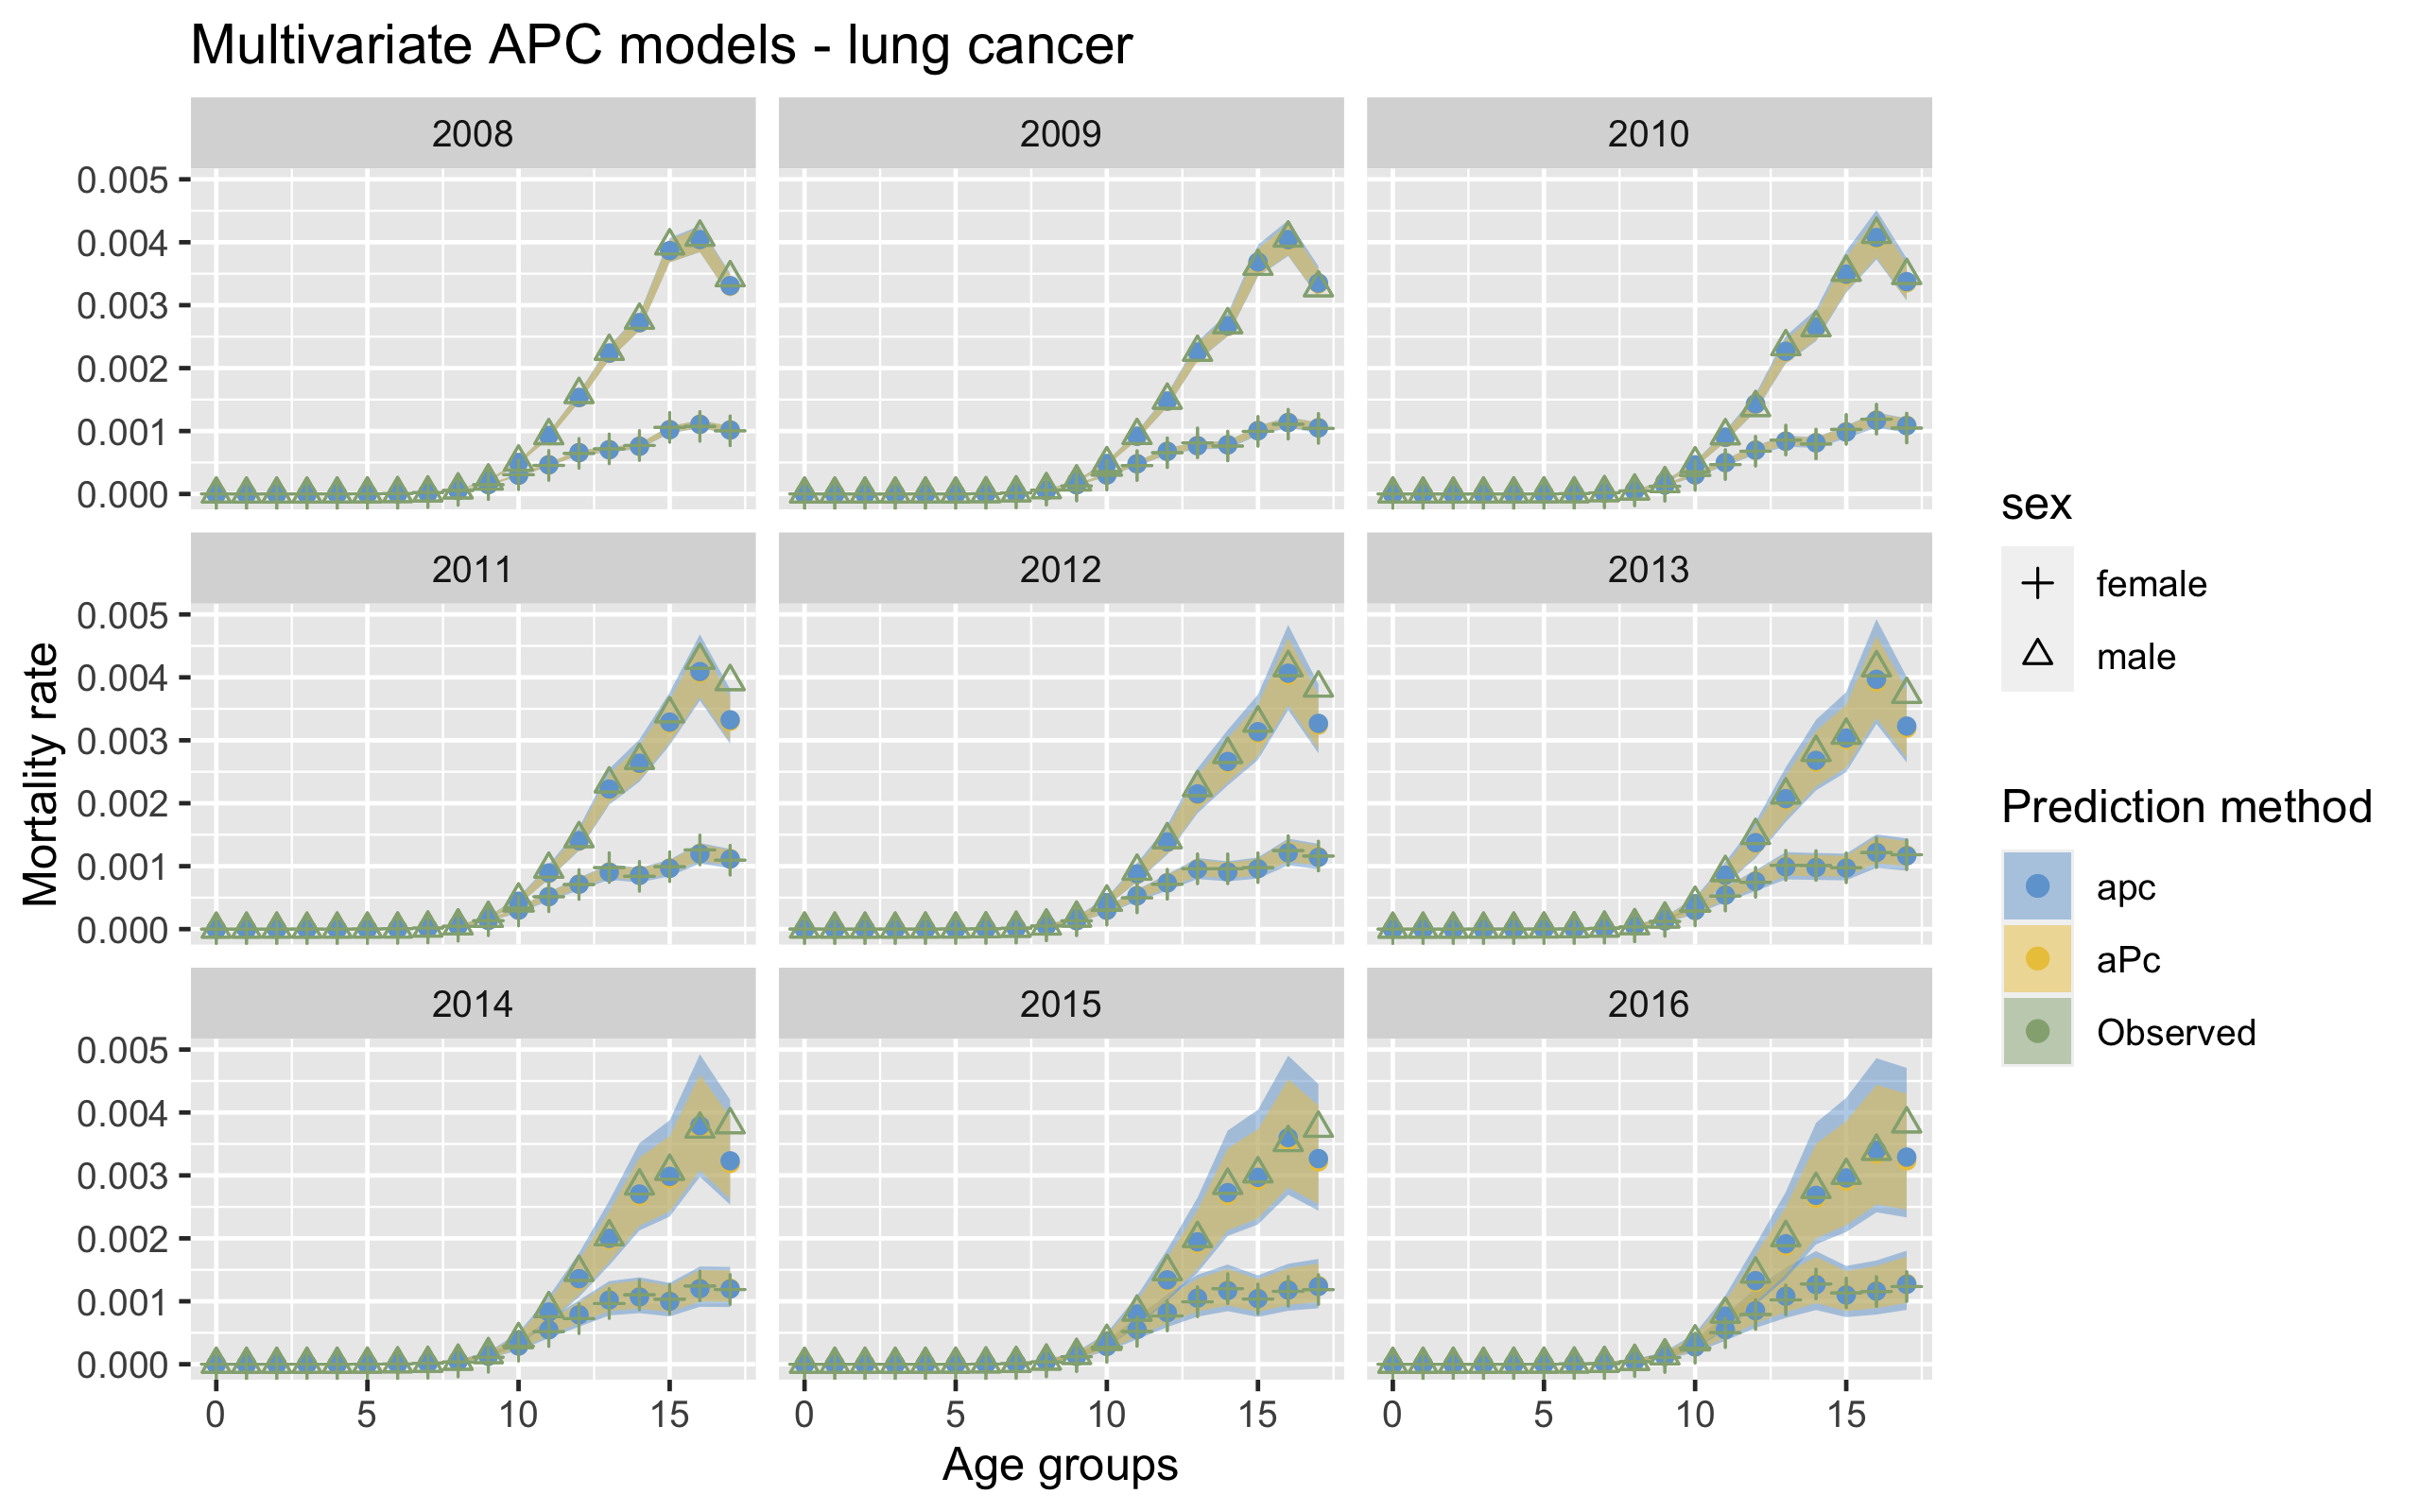
\includegraphics[width=\linewidth]{real-data/real-data-multivariate/Figures/multivariate-APC-by-age-lung.png}
    \end{subfigure}
    \begin{subfigure}[b]{.45\linewidth}
        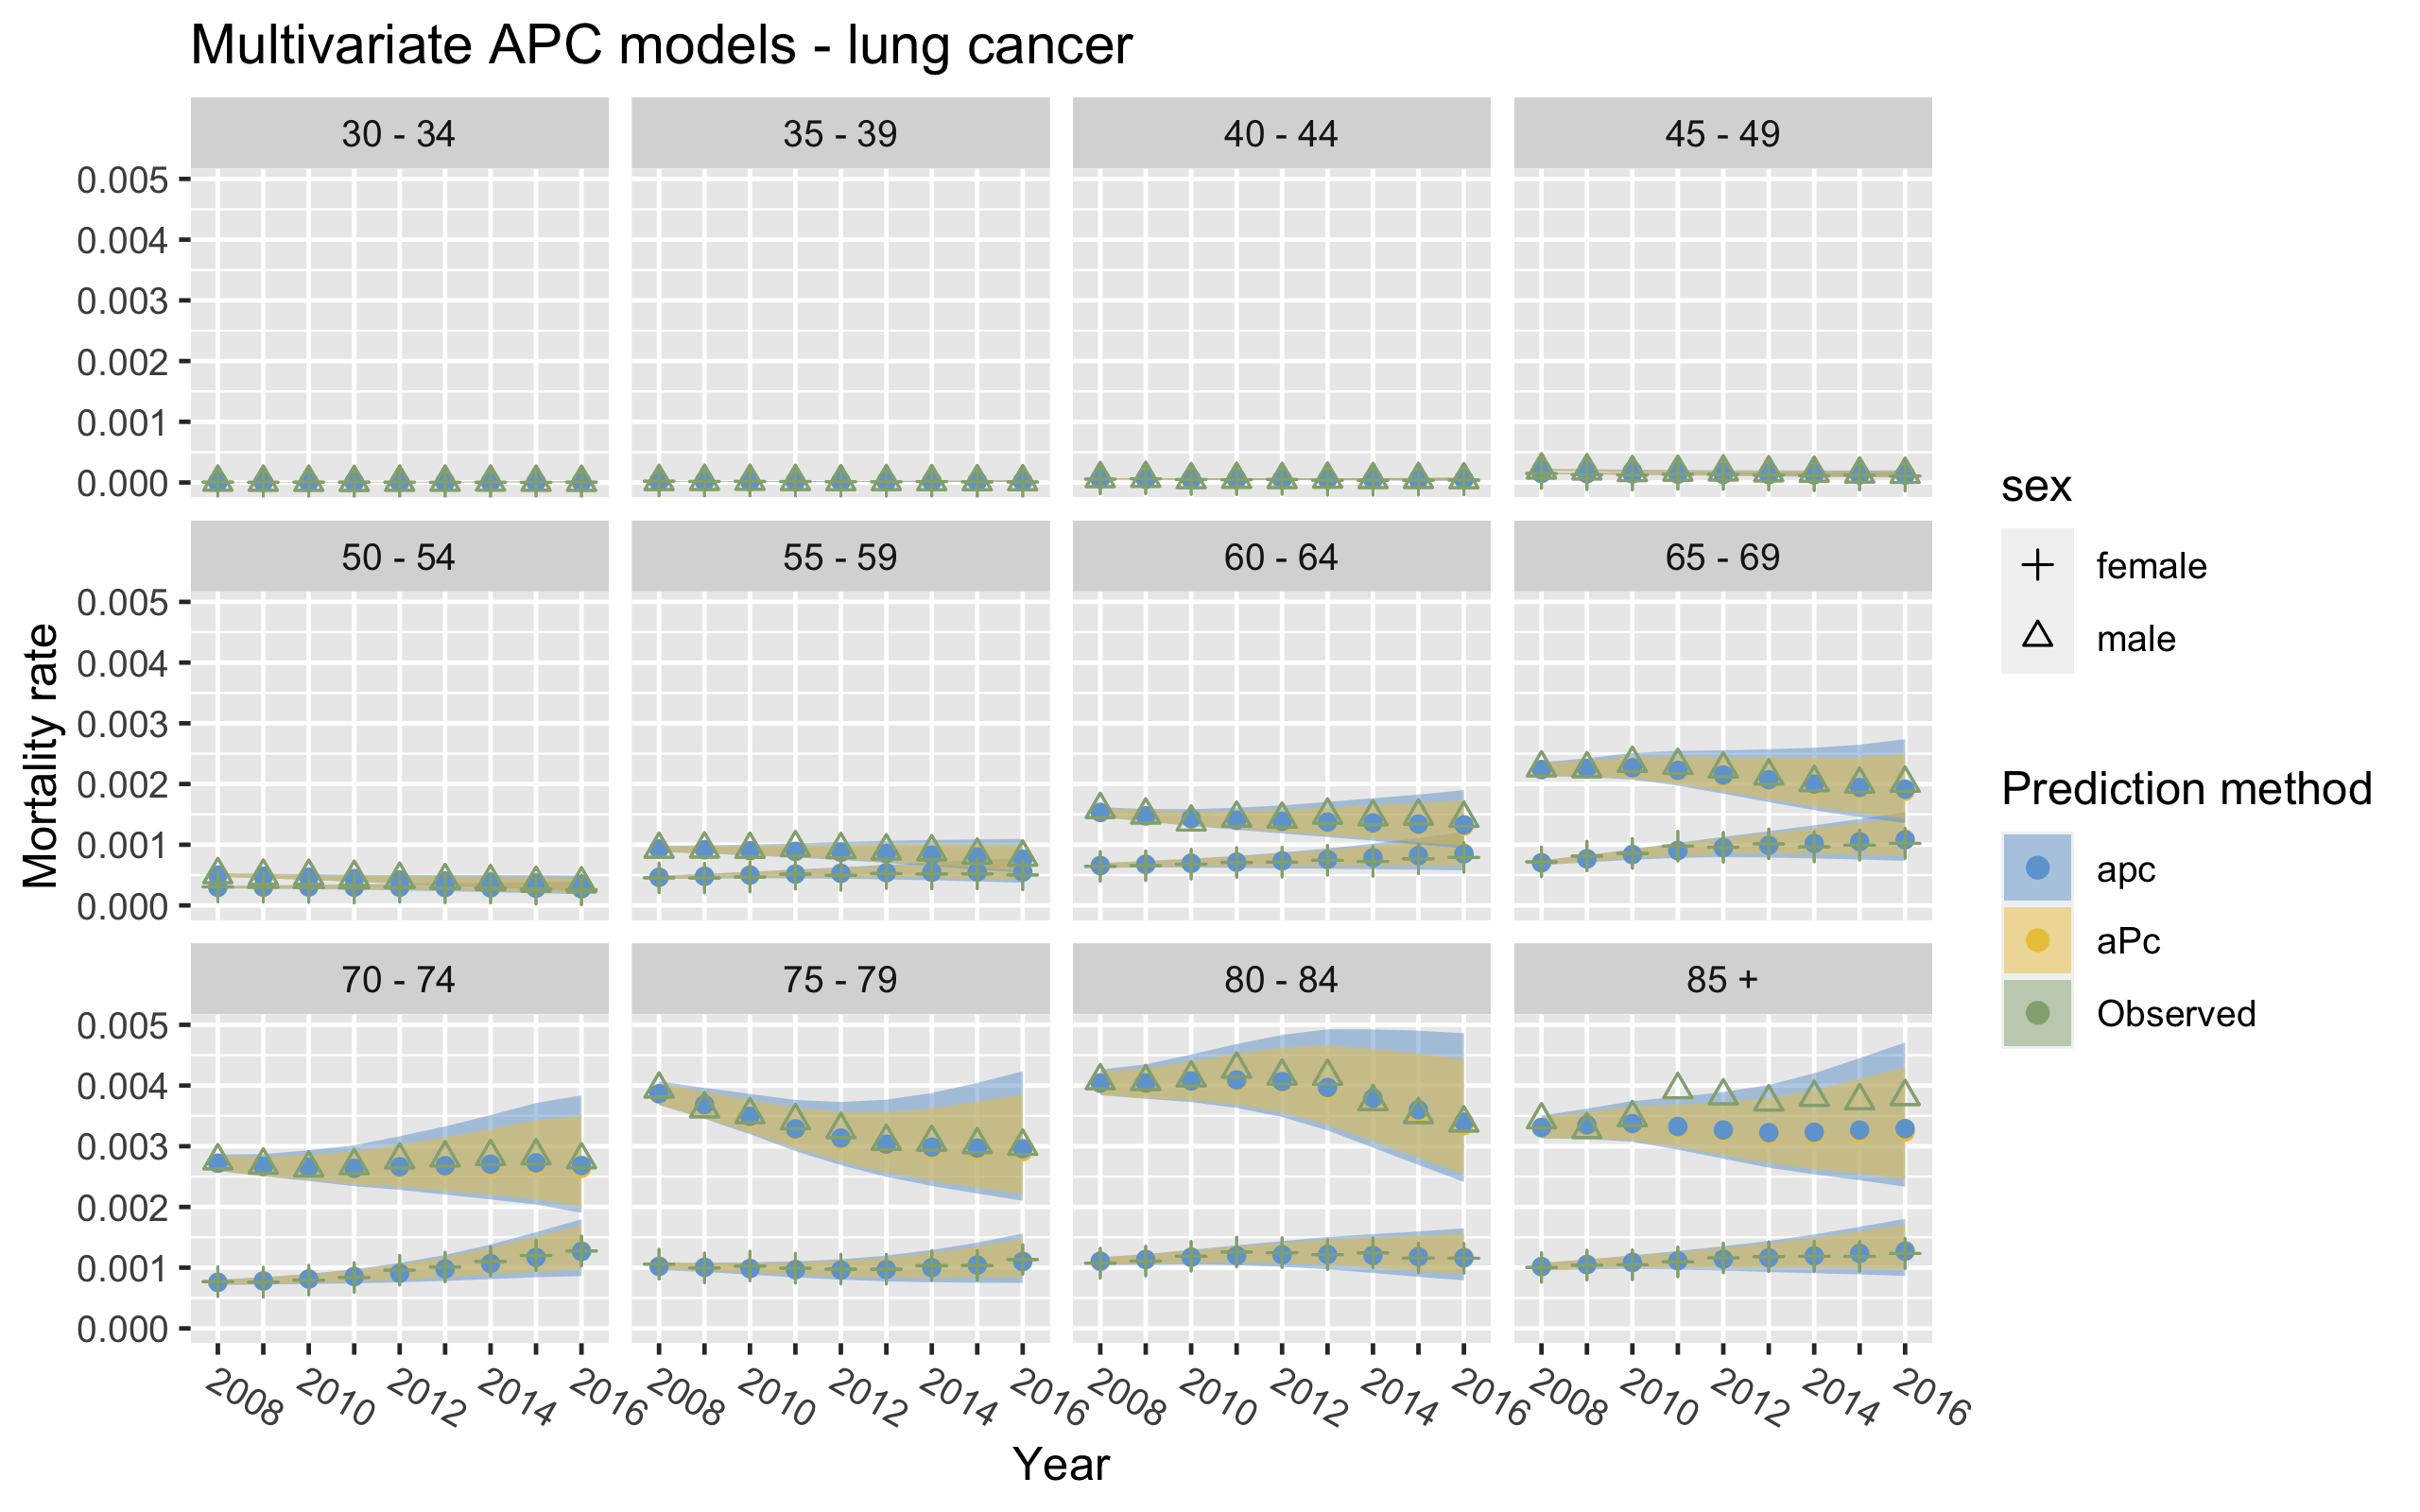
\includegraphics[width=\linewidth]{real-data/real-data-multivariate/Figures/multivariate-APC-by-period-lung.png}
    \end{subfigure}
    \caption{The two best APC models - by age (left) and period (right) for the lung cancer data set}
    \label{fig:mv-APC-lung}
\end{figure}

\begin{figure}[h!]
    \centering
    \begin{subfigure}[b]{.45\linewidth}
        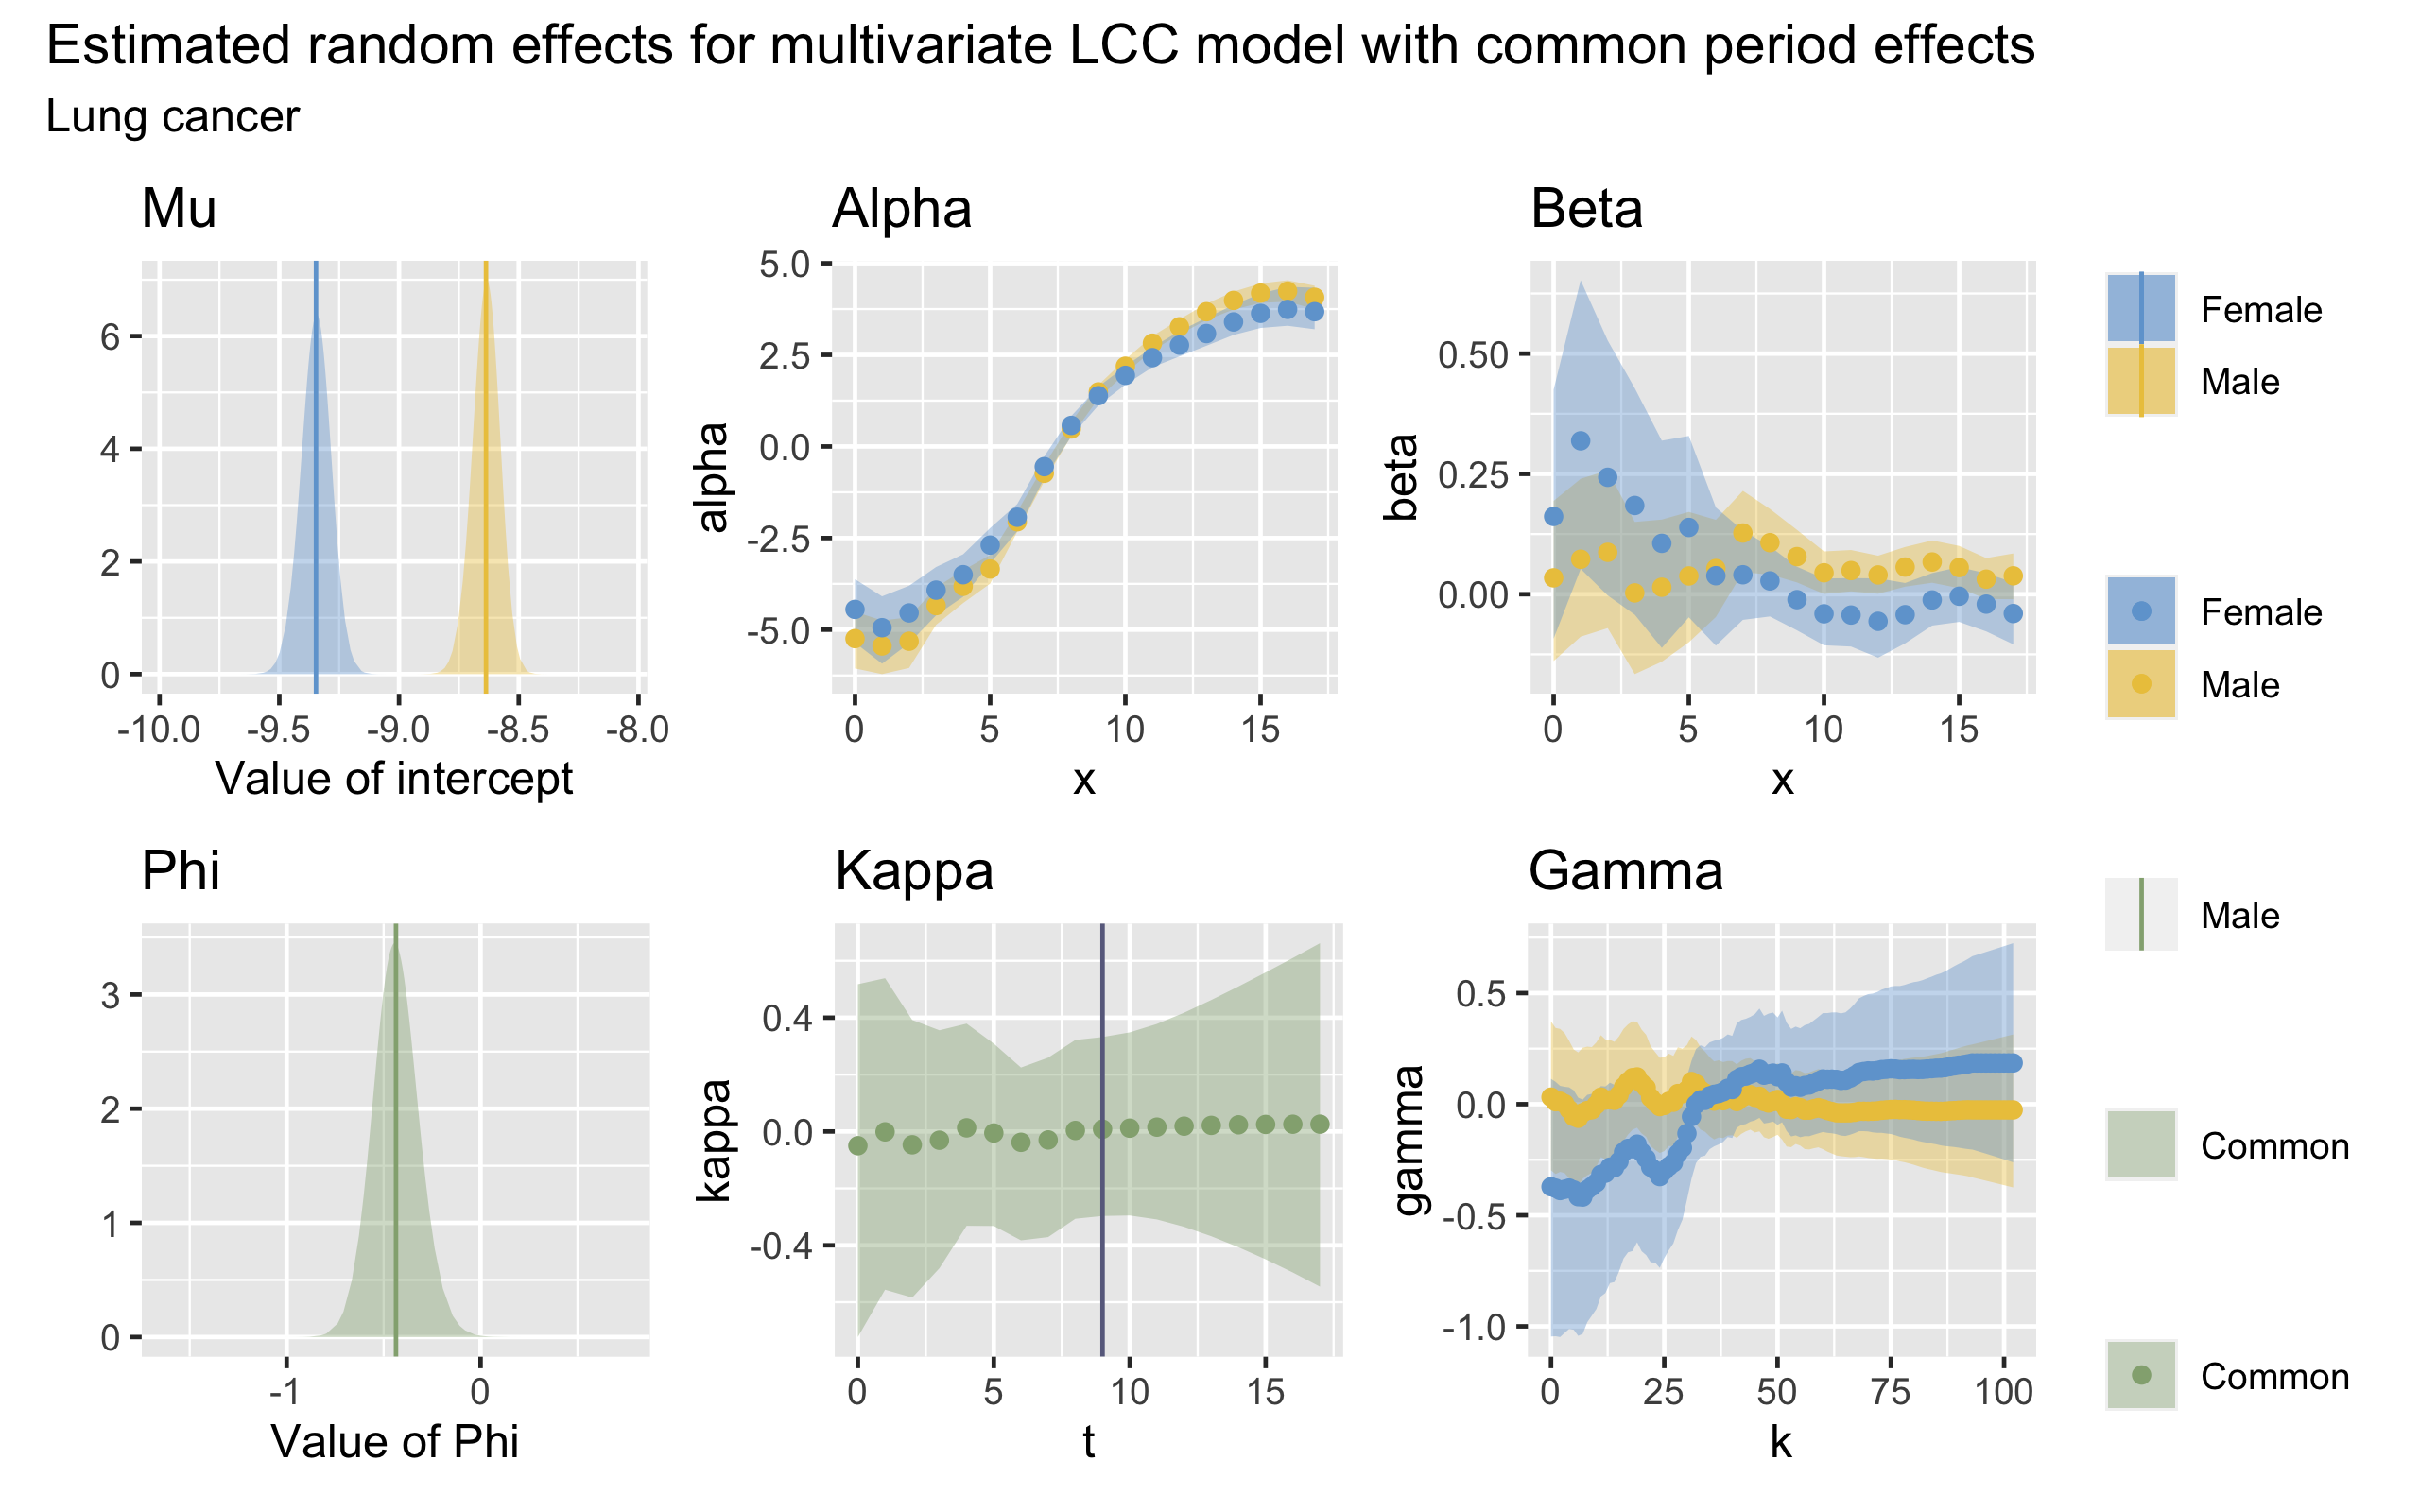
\includegraphics[width=\linewidth]{real-data/real-data-multivariate/Figures/effects-LCC-common-period-lung.png}
    \end{subfigure}
    \begin{subfigure}[b]{.45\linewidth}
        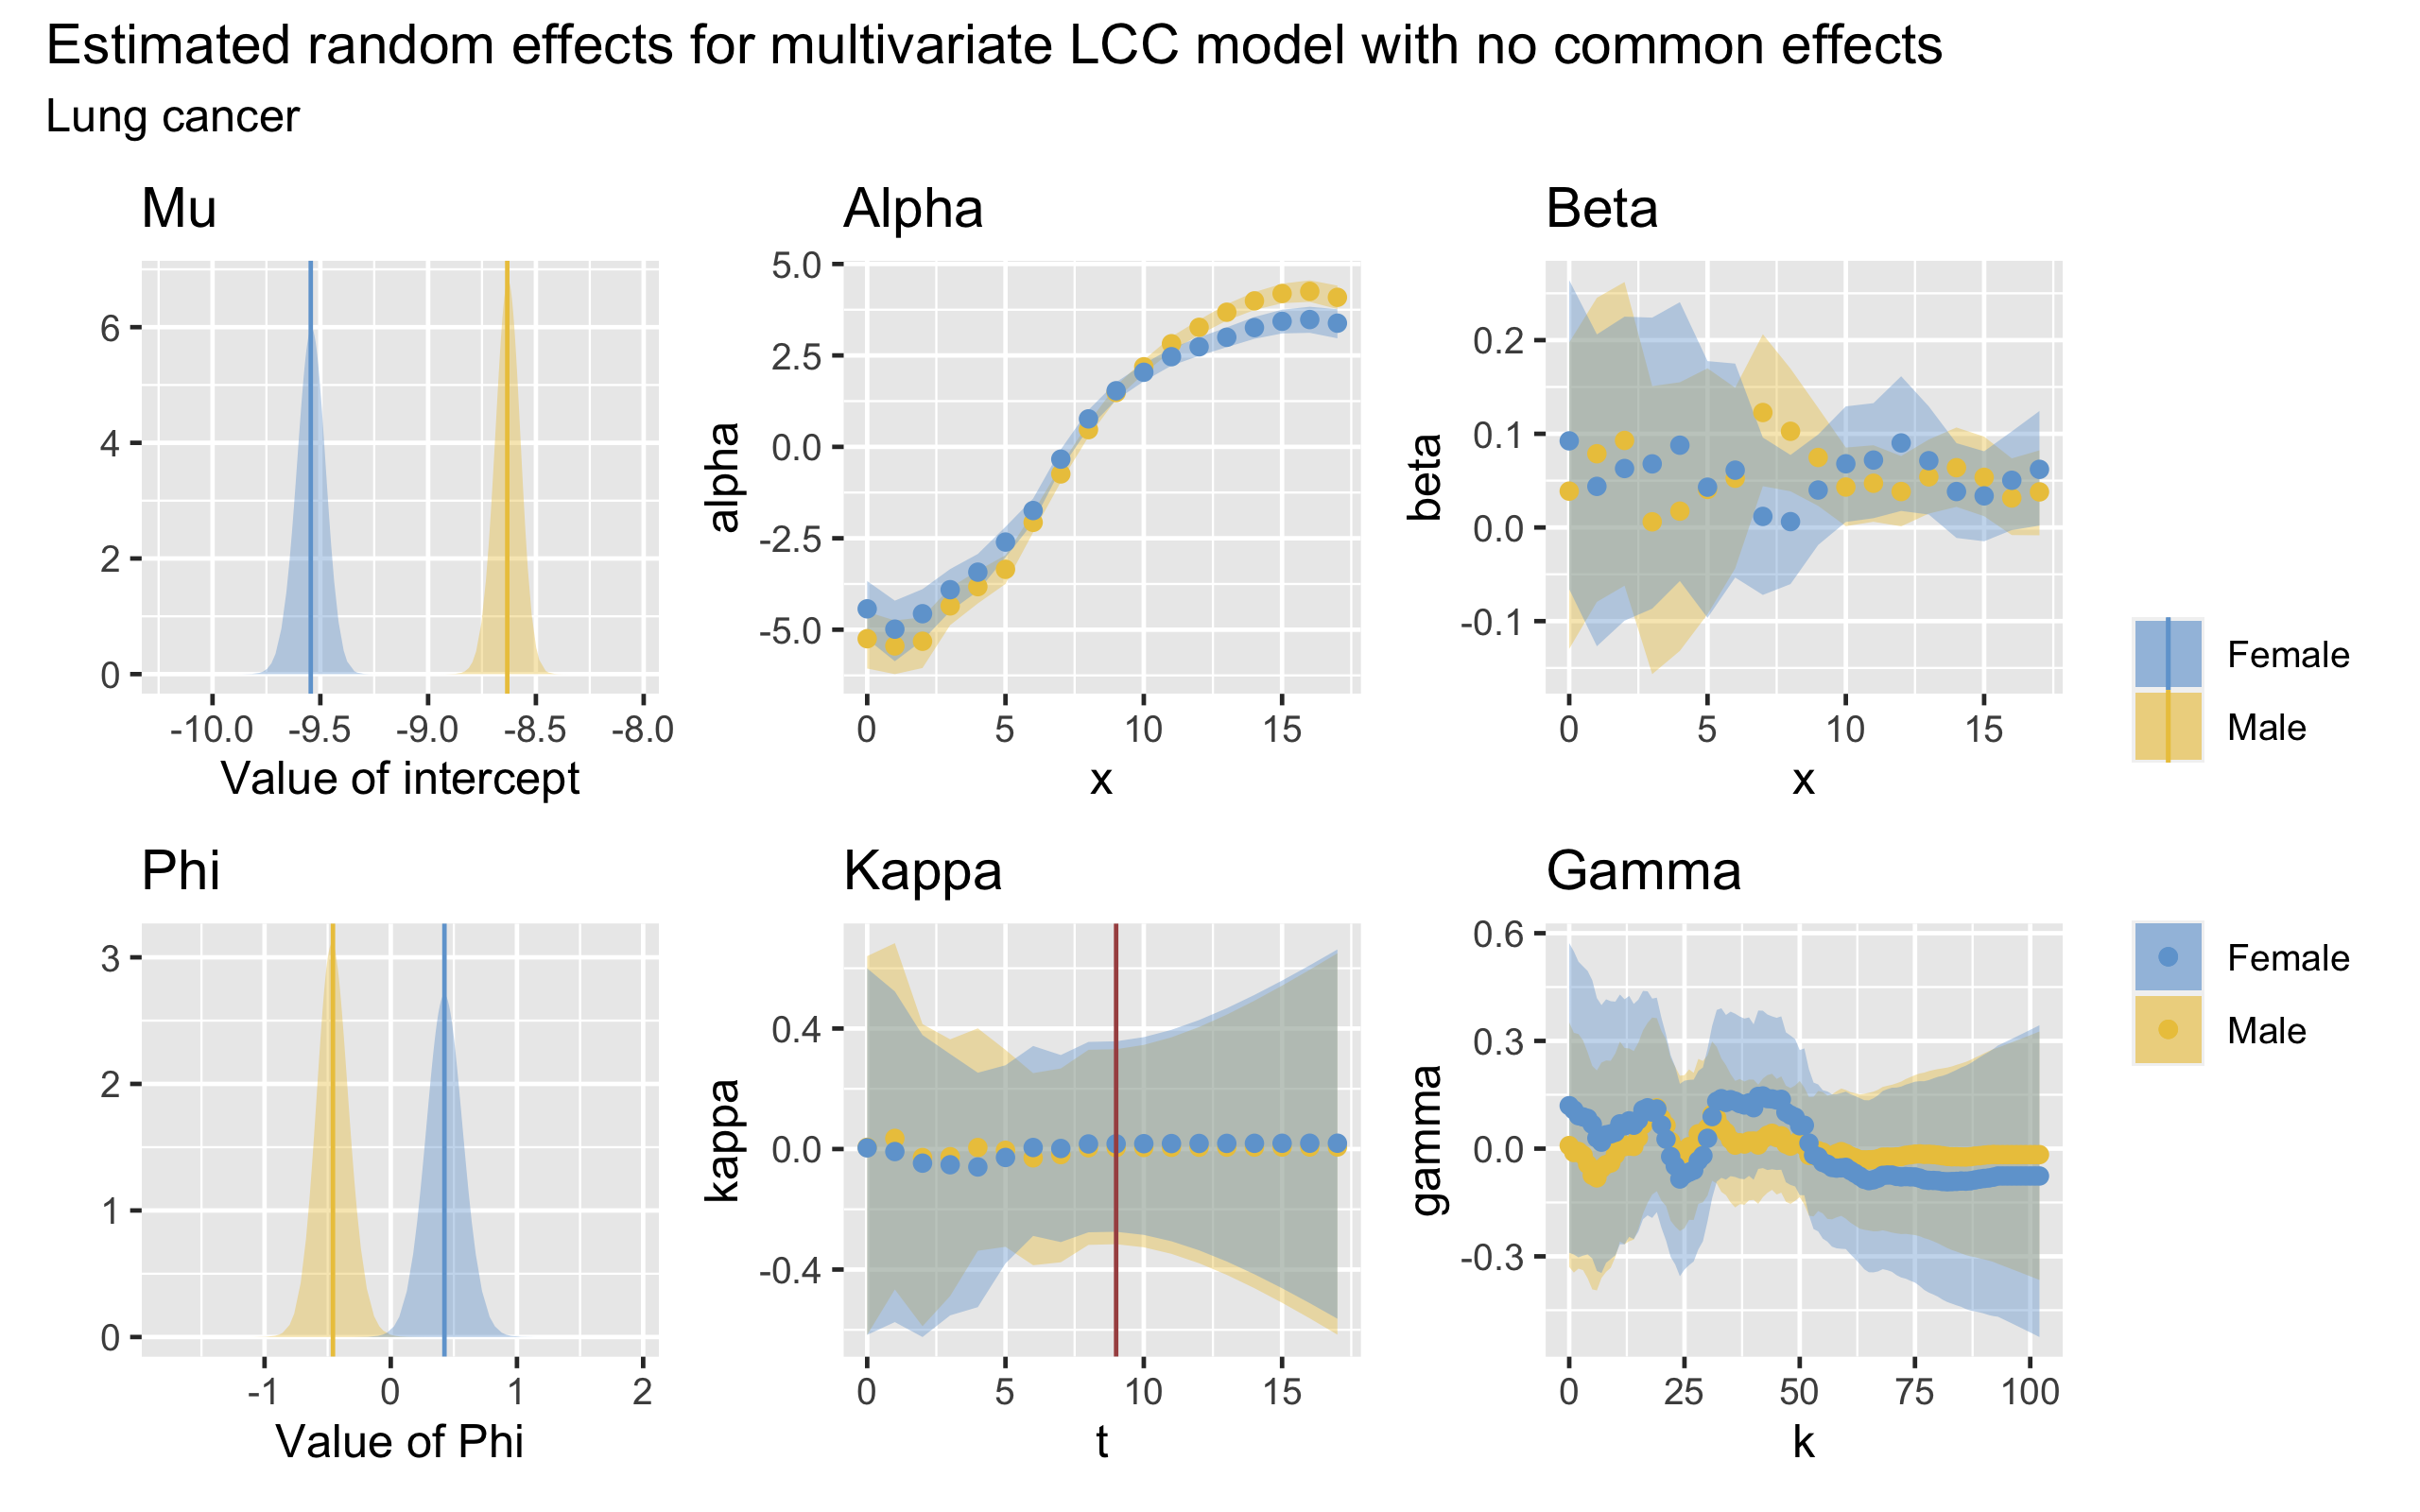
\includegraphics[width=\linewidth]{real-data/real-data-multivariate/Figures/effects-LCC-no-common-lung.png}
    \end{subfigure}
    \caption{Plots of the effects for the two best LCC models - LCC with common period effects (left) and LCC with no common effects (right) for the lung cancer data}
    \label{fig:effects-LCC-lung}
\end{figure}

\begin{figure}[h!]
    \centering
    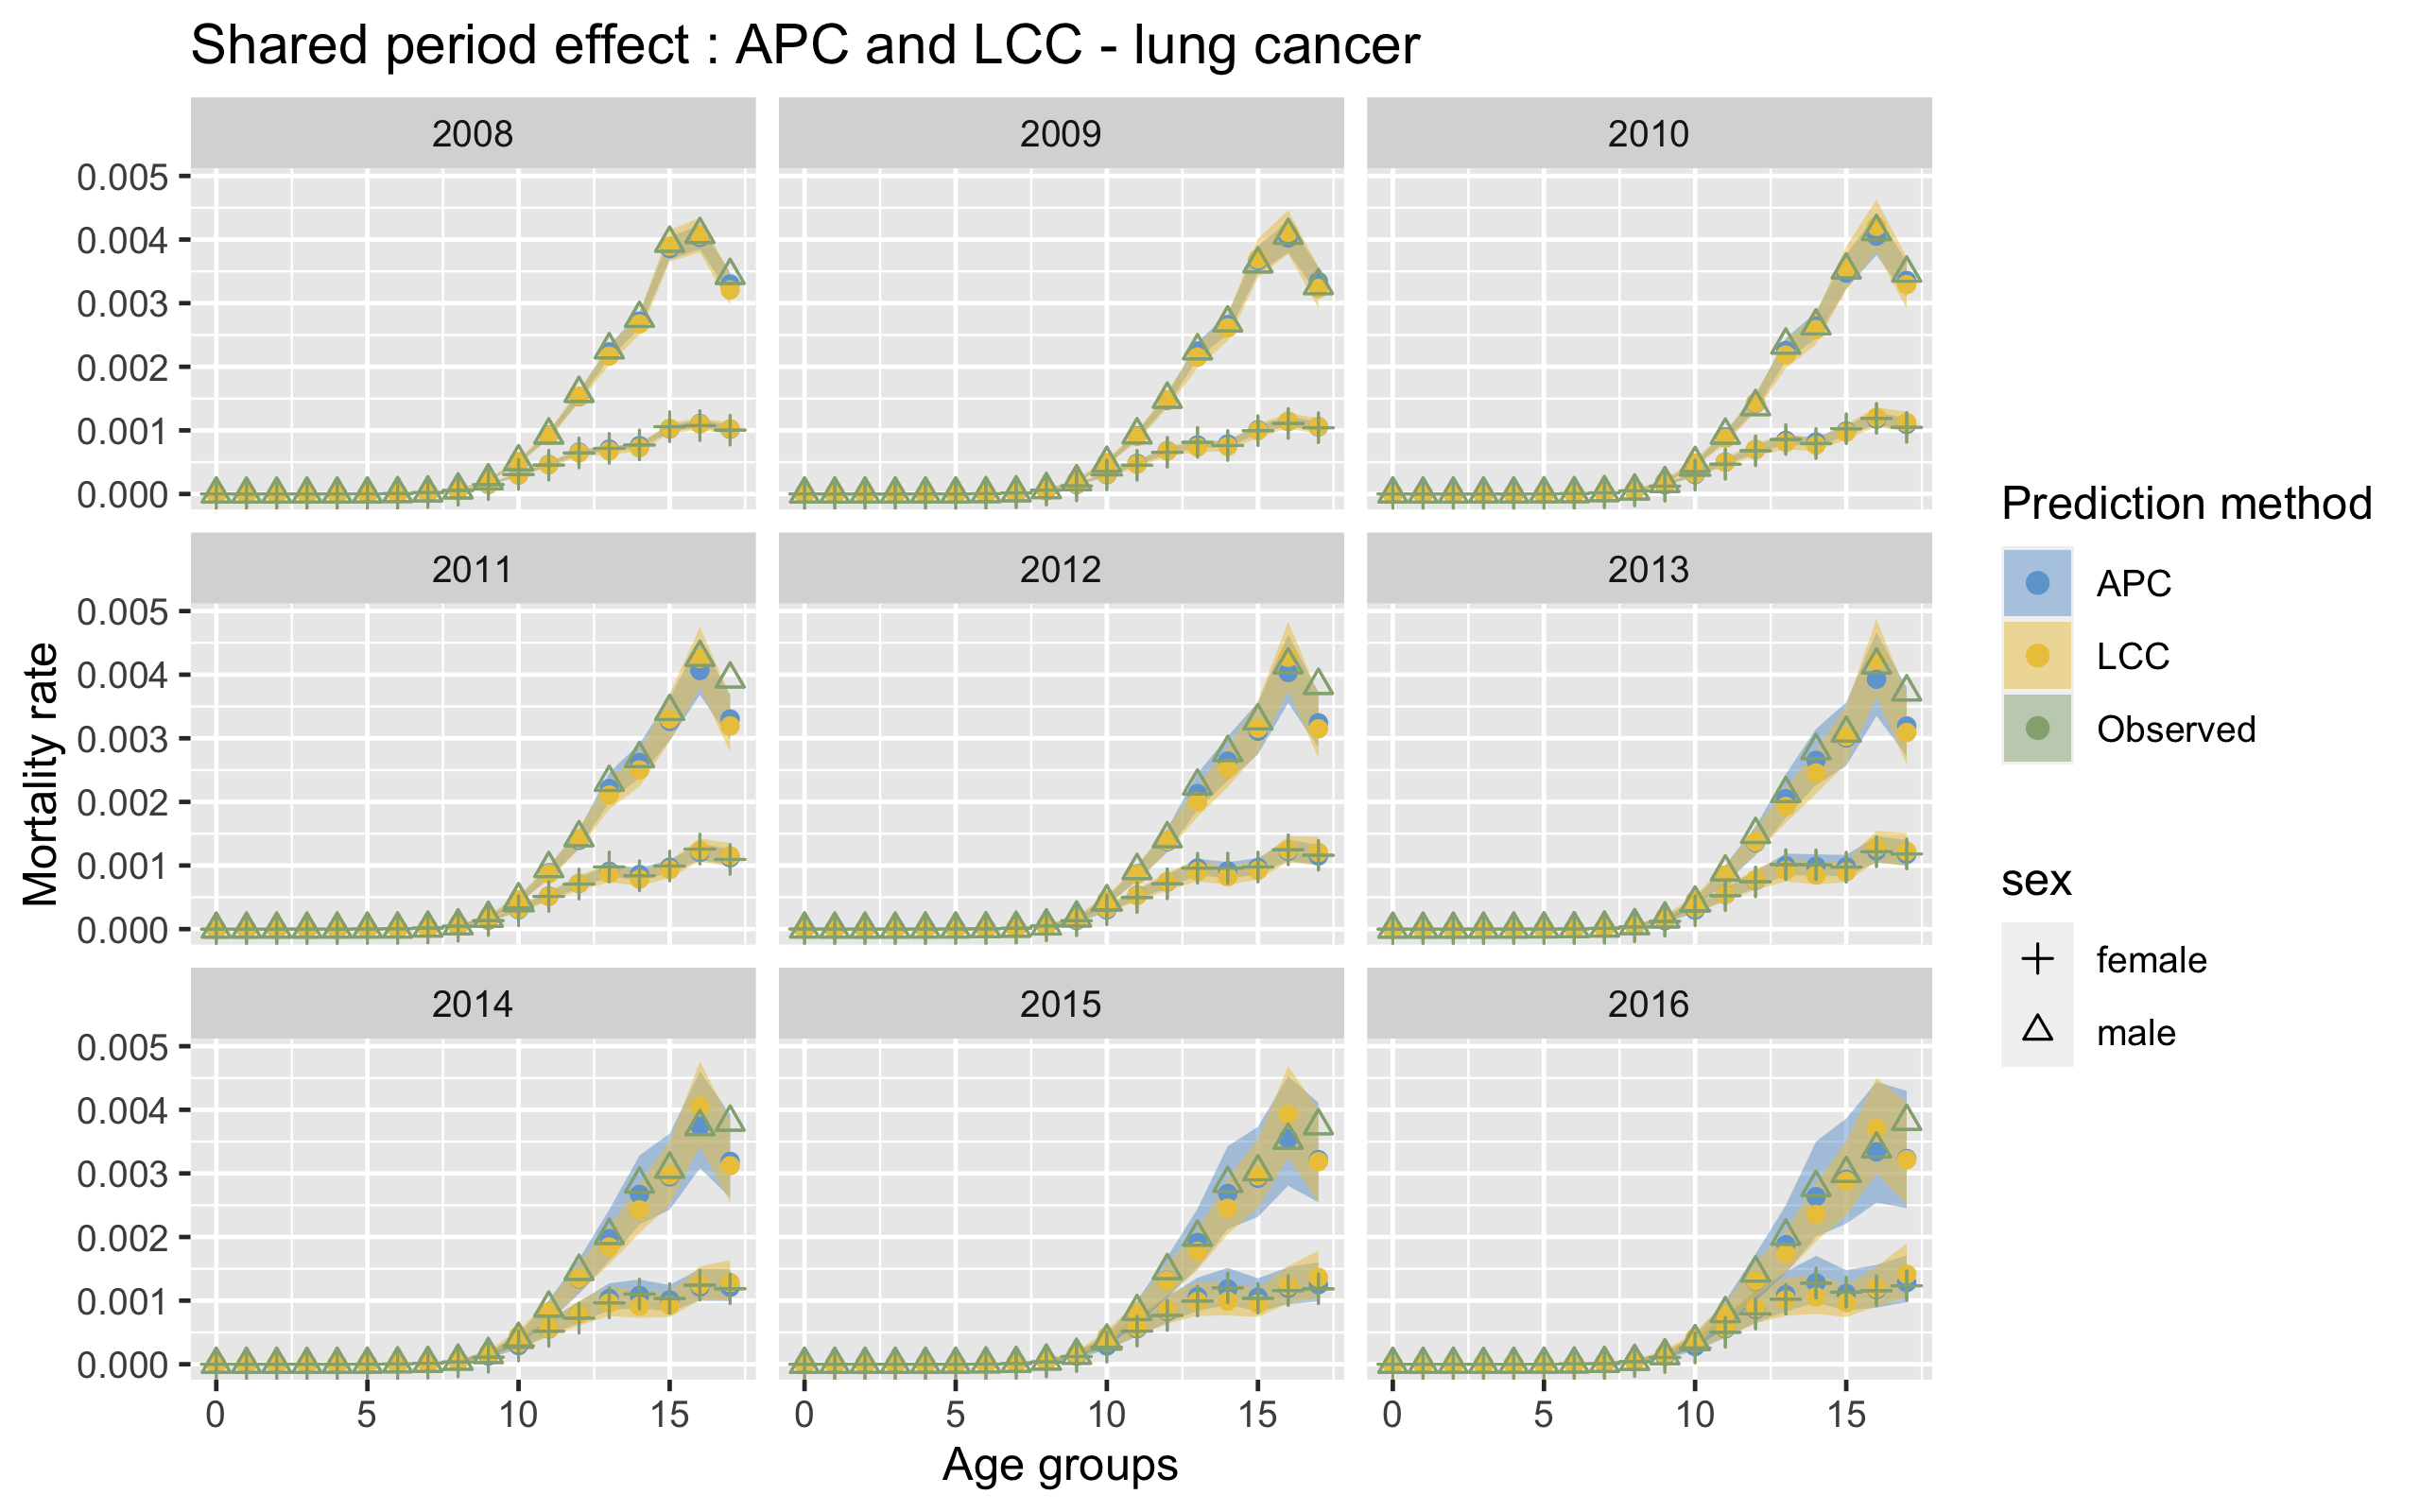
\includegraphics[width = .8\linewidth]{real-data/real-data-multivariate/Figures/multivariate-comparison-by-age-lung.png}
    \caption{Comparison of the best APC model and the best LCC model - by age}
    \label{fig:mv-LCC-by-period-lung}
\end{figure}

\begin{figure}[h!]
    \centering
    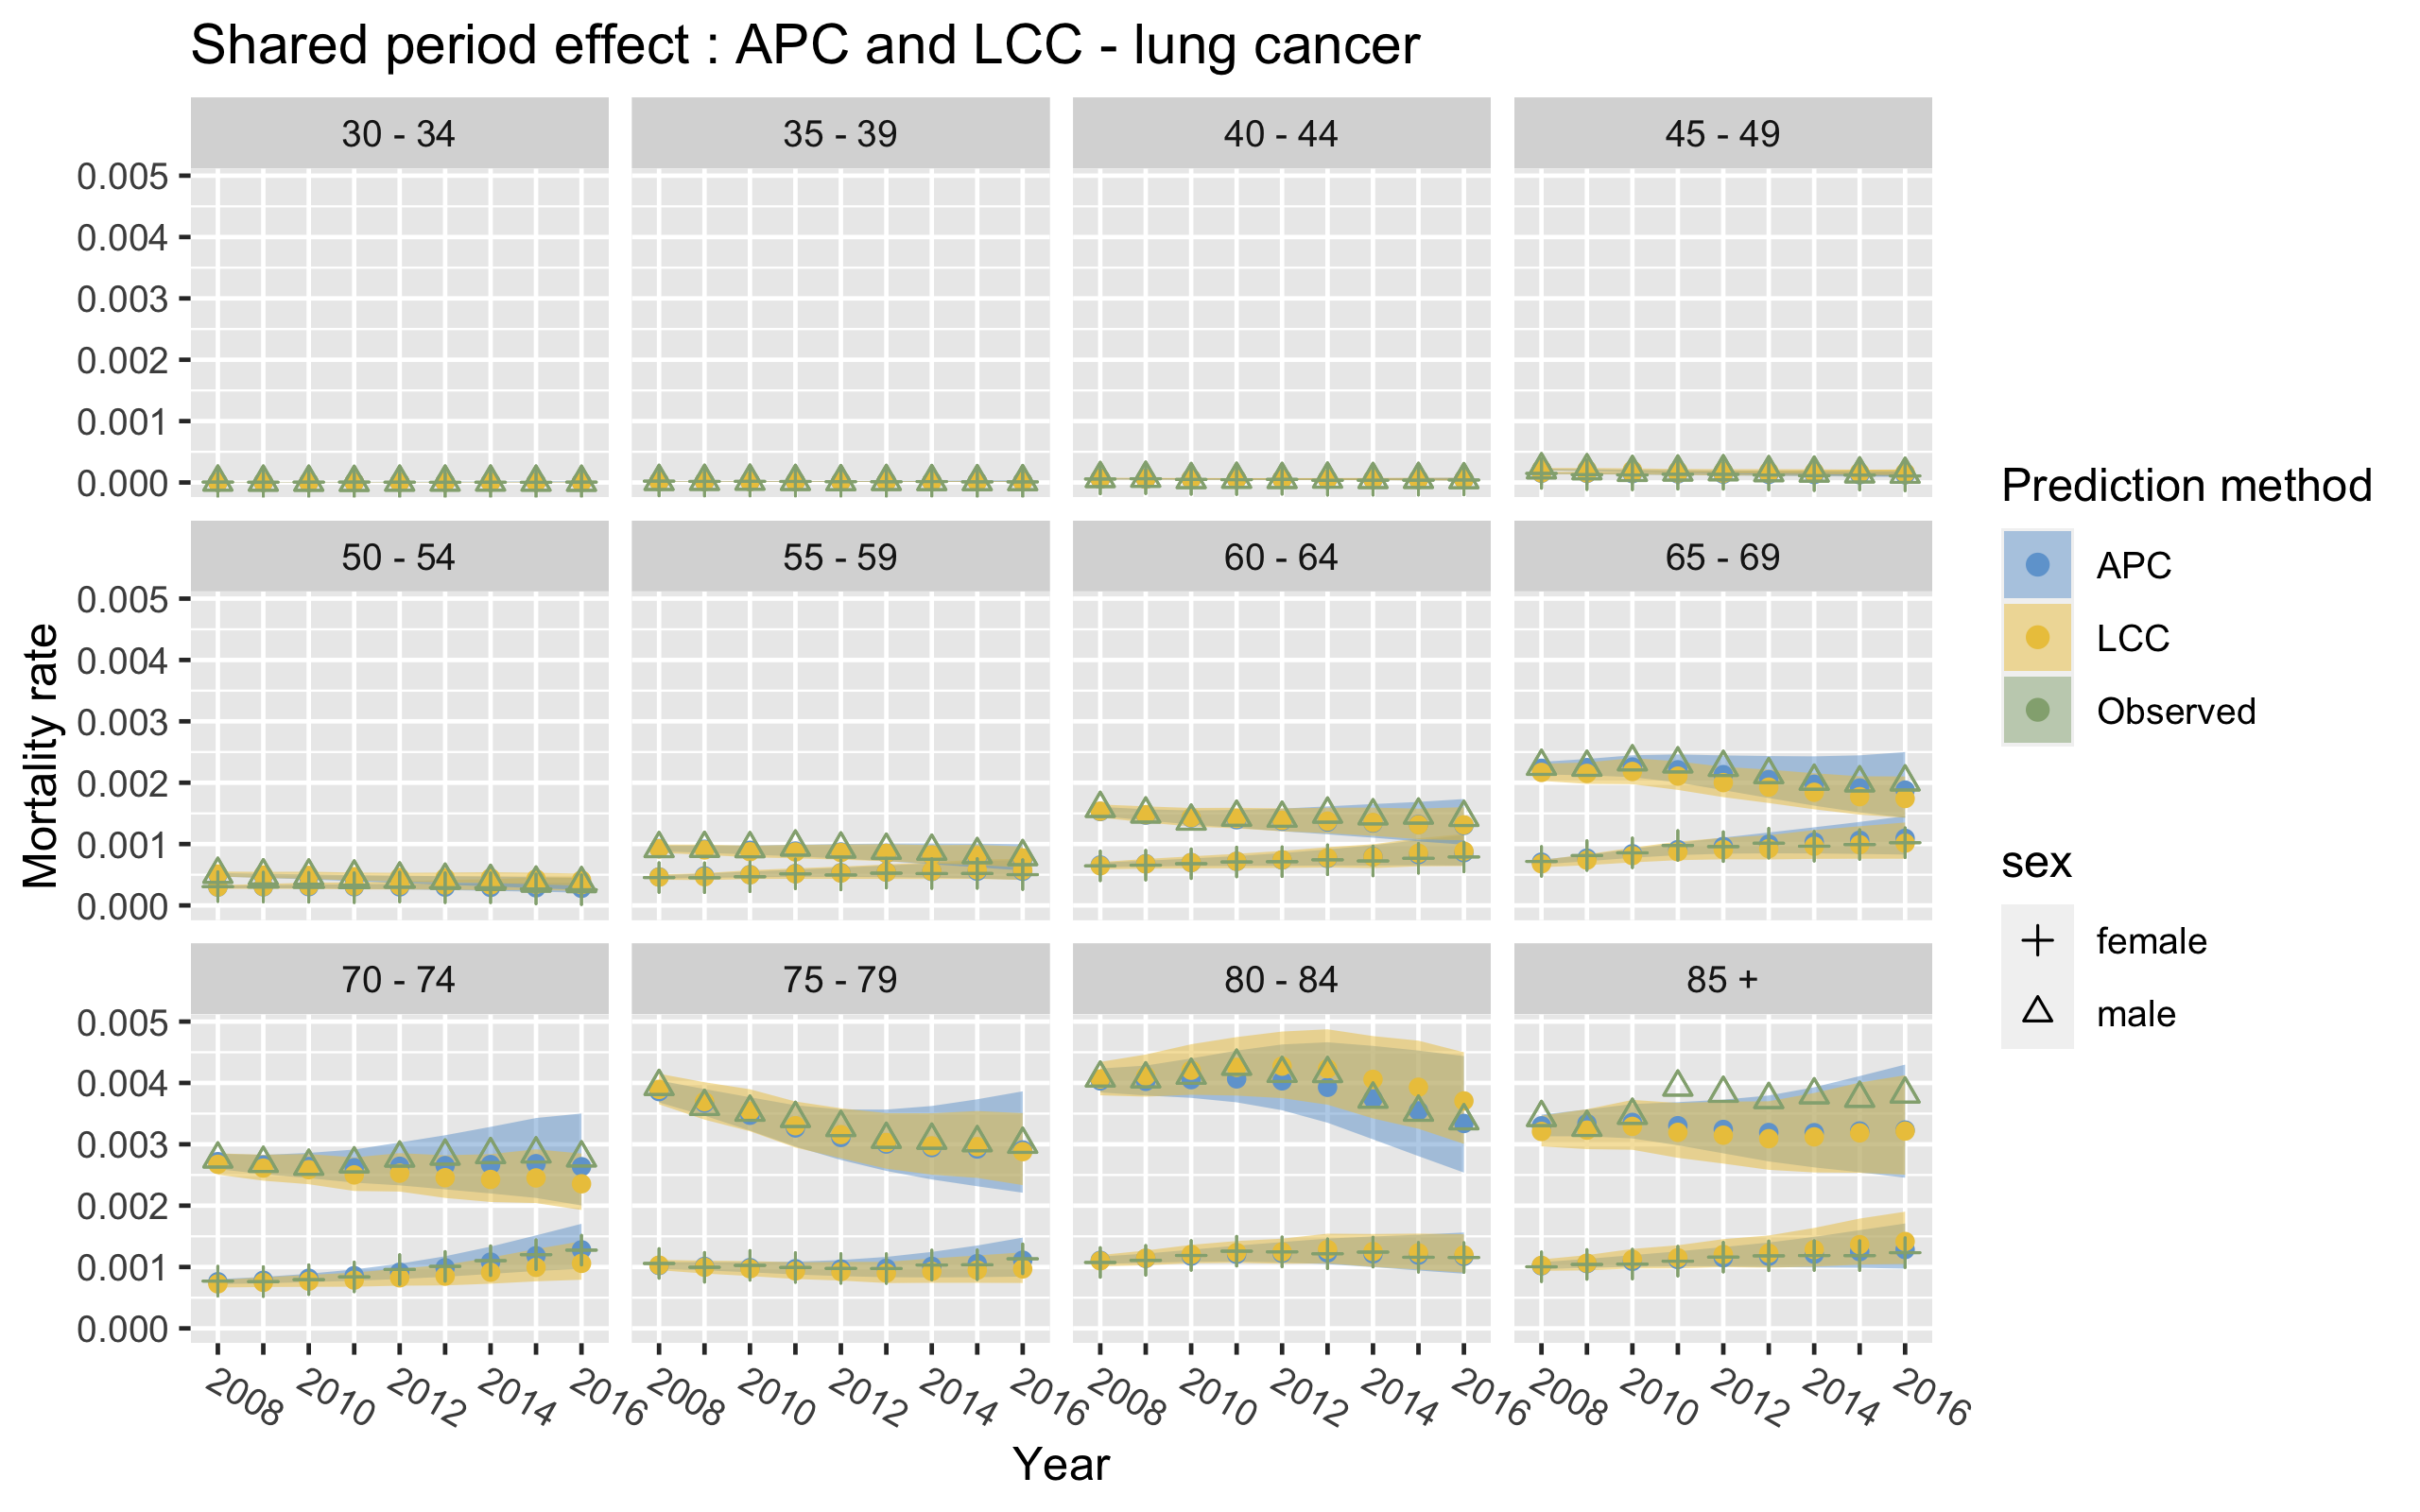
\includegraphics[width = .8\linewidth]{real-data/real-data-multivariate/Figures/multivariate-comparison-by-period-lung.png}
    \caption{Comparison of the best APC model and the best LCC model - by period}
    \label{fig:mv-APC-by-period-lung}
\end{figure}


\begin{table}[h!]
    \begin{tabular}{l |c c c }
        Model & MSE & MDSS & Contained 95\%-interval\\
        \hline
        apc    & 1.033e-8 & \textbf{-19.74} (-21.64)    & 0.9120 \\
        apC    & 2.437e-8 & -19.07 (-20.80)   & 0.8843 \\
        aPc    & 1.238e-8 & \textbf{-19.83} (-21.68)   & 0.9028 \\
        aPC    & 7.472e-8 & -17.70 (-20.09)   & 0.8889 \\
        Apc    & 6.709e-9 & -19.21 (-21.24)   & 0.8981 \\
        ApC    & 1.672e-7 & -15.81 (-18.83)   & 0.9954 \\
        APc    & 2.884e-8 & -18.71 (-20.96)   & 0.875  \\
        APC    & 9.055e-8 & -16.19 (-18.89)   & 0.9676 \\
    \end{tabular}
    \caption{\label{tab:APC-lung}Score statistics for the different multivariate APC models, for the lung cancer data set. The lowest mean DSS values are marked in bold font. }
\end{table}

\newpage
\subsubsection{Stomach cancer data}
\textcolor{myDarkGreen}{Så og si samme tekst og plott som for lung cancer - med andre diskusjoner dersom det oppstår}

\begin{table}[h!]
    \begin{tabular}{l |c c c }
        Model & MSE & MDSS & Contained 95\%-interval\\
        \hline
        All common            & 1.019e-7  & -17.04    & 0.9769 \\
        Common age            &  9.69e-8 & -17.92    & 0.7454 \\
        Common age, cohort    & 8.969e-8 & -16.93    & 0.7546 \\
        Common age, period    & 5.991e-8 & -18.04    & 0.8565 \\
        Common cohort         &  3.544e-8 & -18.13   & 0.8333 \\
        Common period         &  4.962e-8 & \textbf{-18.78}   & 0.875  \\
        Common period, cohort & 3.631e-8 & -18.01    & 0.8426 \\
        No shared             &  4.929e-8 & \textbf{-18.71}    & 0.8611 \\
    \end{tabular}
    \caption{\label{tab:LCC-stomach}Score statistics for the different multivariate LCC models, for the stomach cancer data set. The lowest mean DSS values are marked in bold font. }
\end{table}

\begin{table}[h!]
    \begin{tabular}{l |c c c }
        Model & MSE & MDSS & Contained 95\%-interval\\
        \hline
        apc    &0.00000002195 &\textbf{-19.32}    &0.9306 \\
        apC    &0.00000005602 &-18.51    &0.8657 \\
        aPc    &0.00000002535 &\textbf{-19.36}    &0.9120 \\
        aPC    &0.00000004120 &-17.57    &0.8611 \\
        Apc    &0.00000001330 &-18.68    &0.9120 \\
        ApC    &0.0000002969  &-15.15    &0.9861 \\
        APc    &0.00000003634 &-18.47    &0.875  \\
        APC    &0.00000008517 &-15.94    &0.9722 \\
    \end{tabular}
    \caption{\label{tab:APC-stomach}Score statistics for the different multivariate APC models, for the stomach cancer data set. The lowest mean DSS values are marked in bold font. }
\end{table}

\begin{figure}[h!]
    \centering
    \begin{subfigure}[b]{.45\linewidth}
        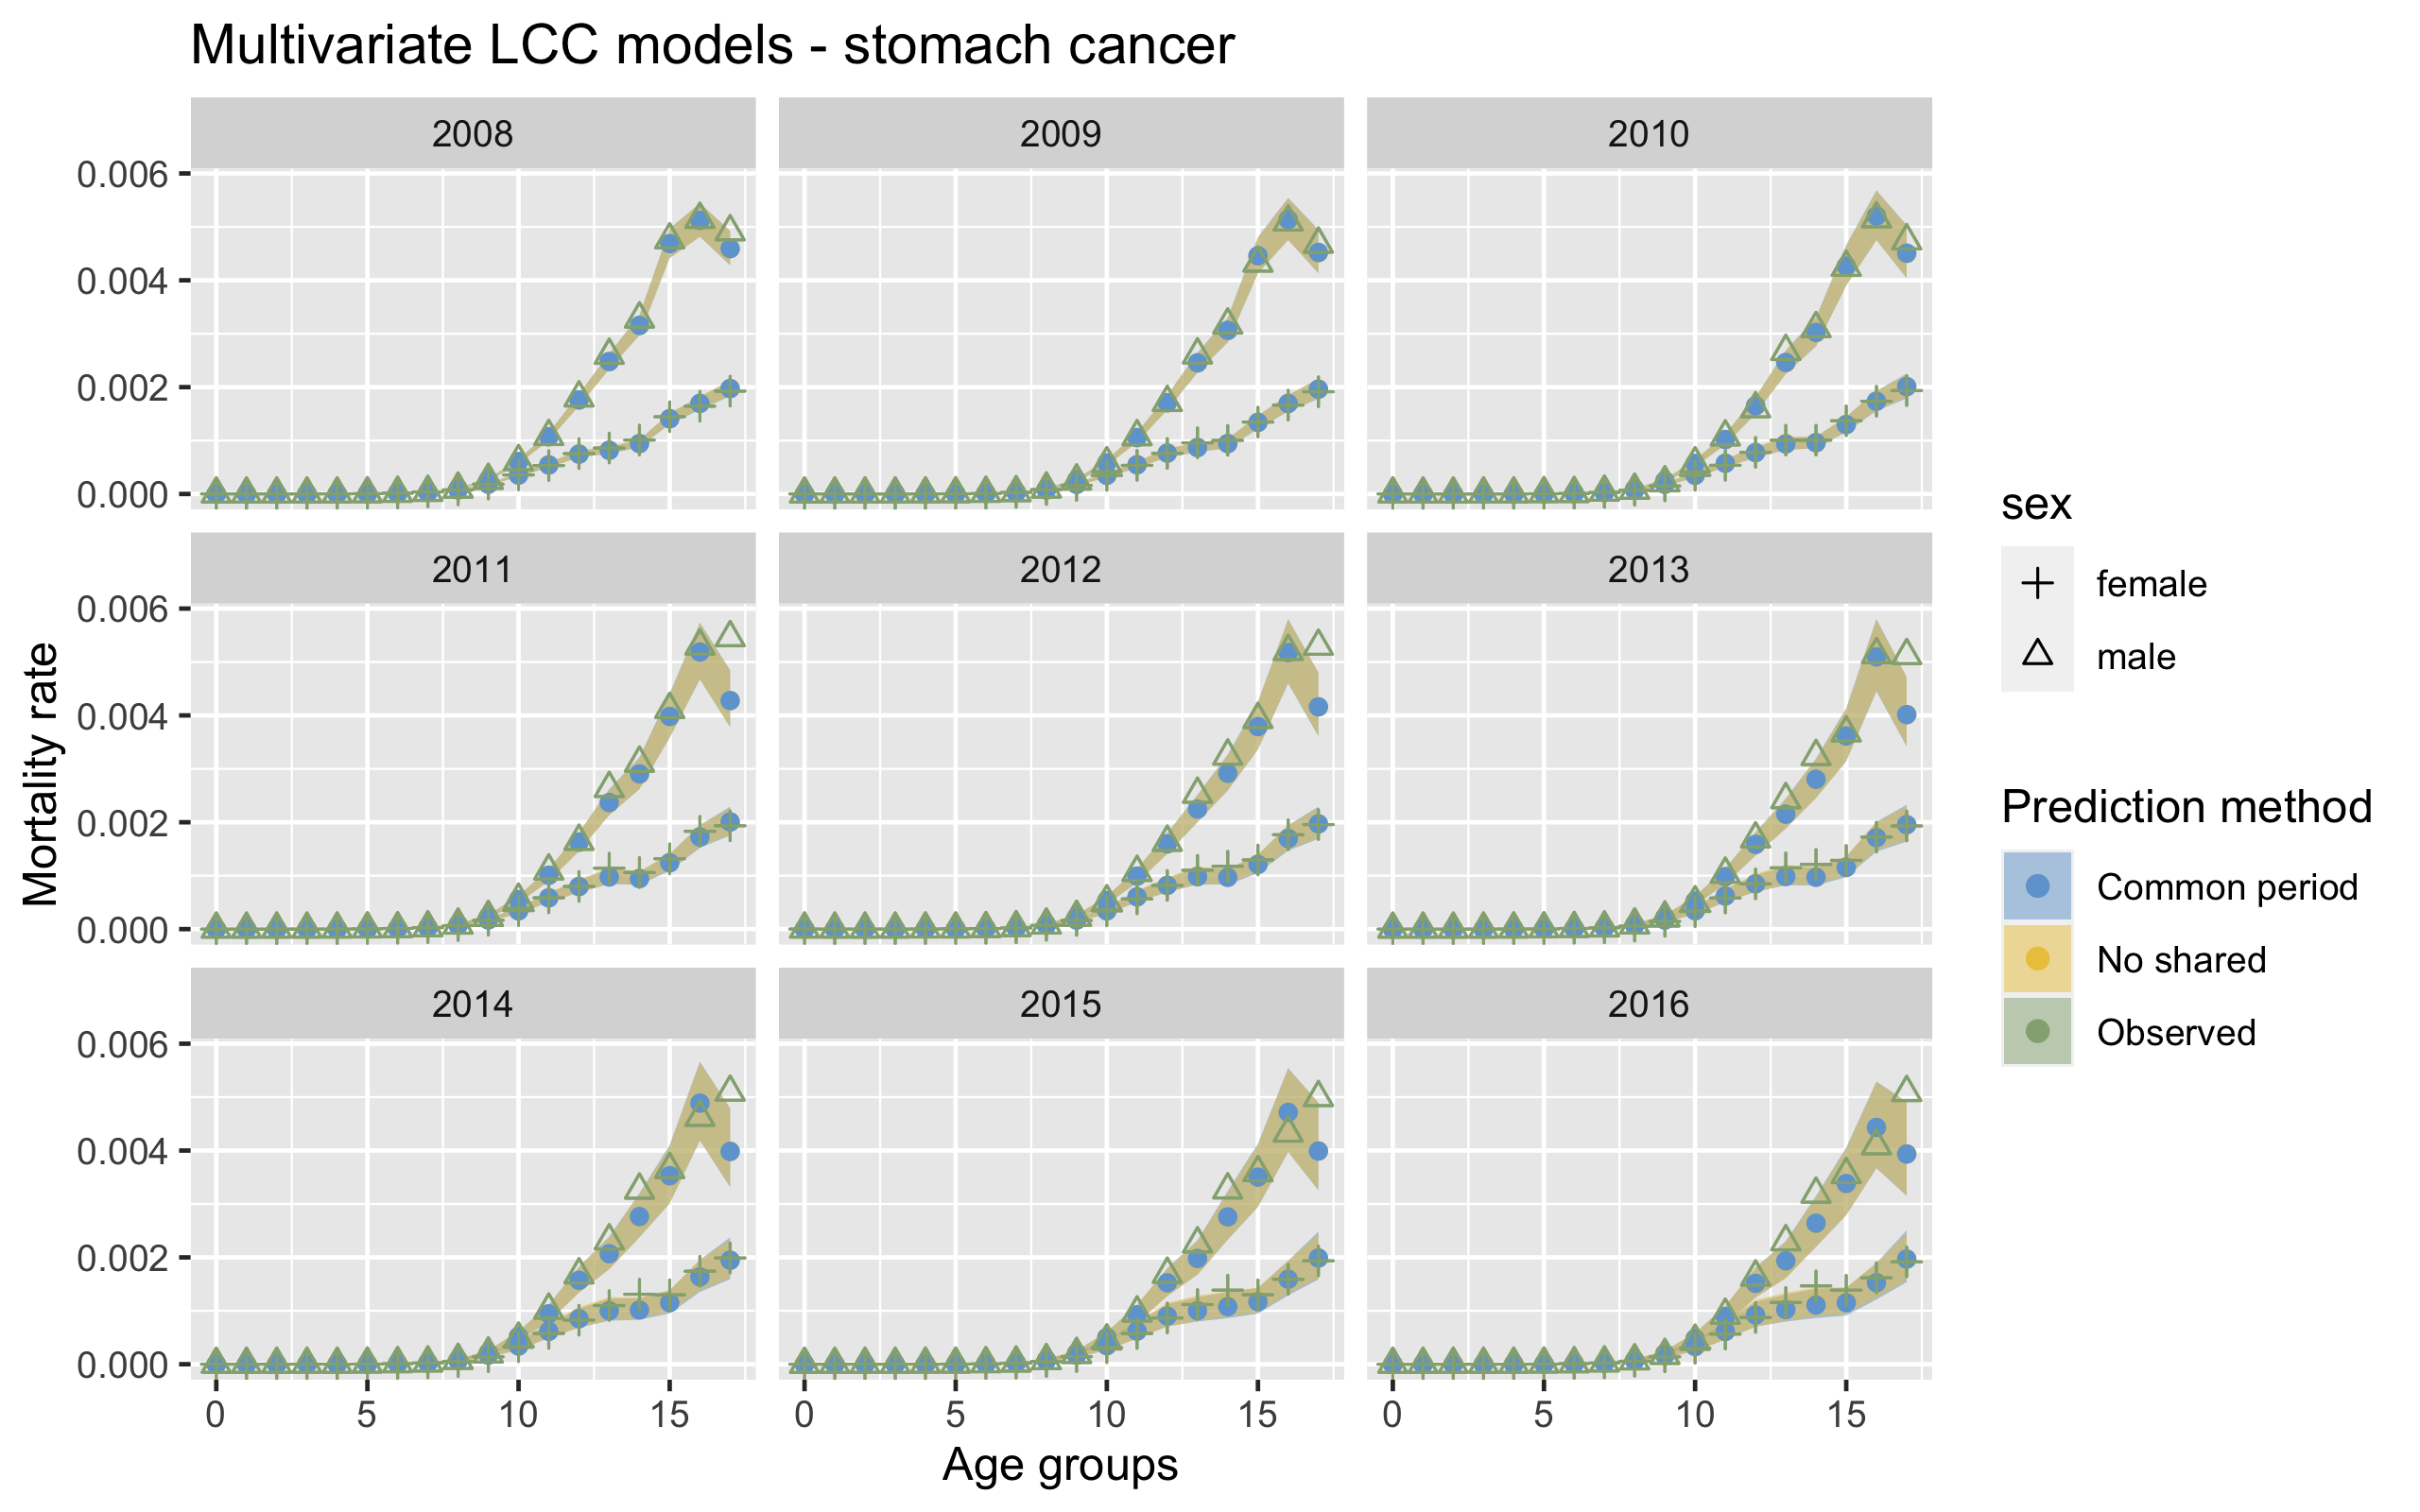
\includegraphics[width=\linewidth]{real-data/real-data-multivariate/Figures/multivariate-LCC-by-age-stomach.png}
    \end{subfigure}
    \begin{subfigure}[b]{.45\linewidth}
        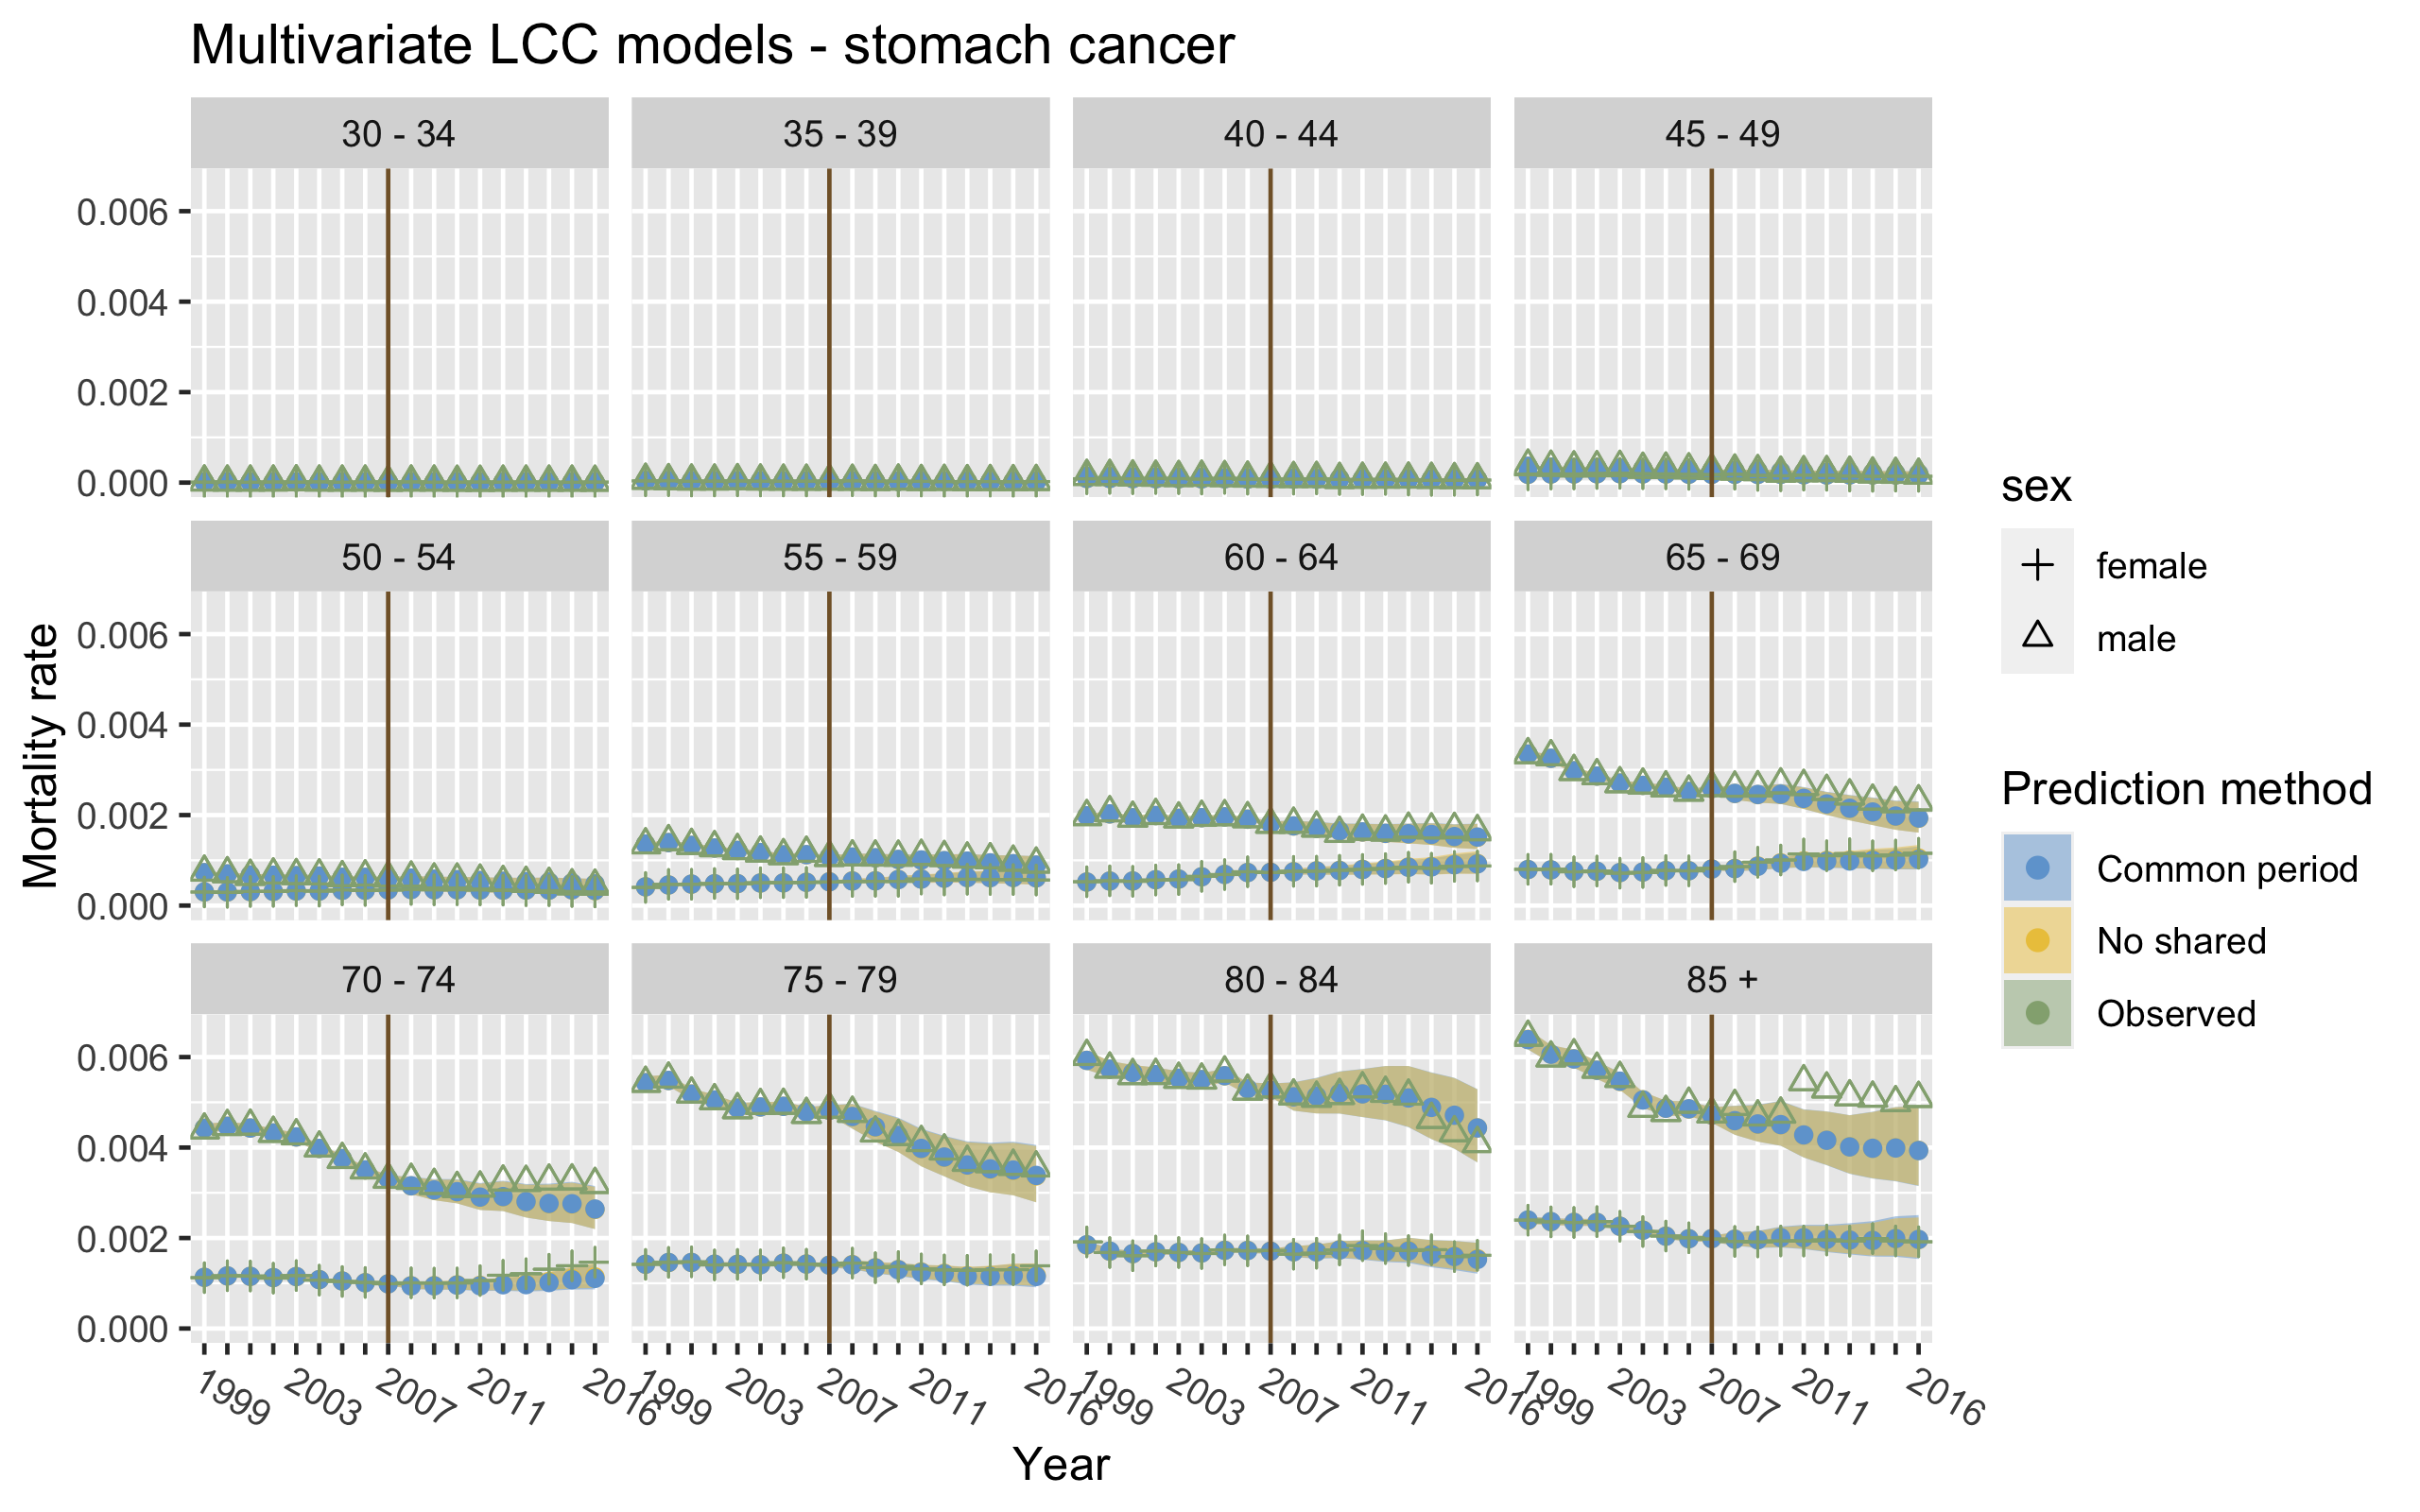
\includegraphics[width=\linewidth]{real-data/real-data-multivariate/Figures/multivariate-LCC-by-period-stomach.png}
    \end{subfigure}
    \caption{The two best LCC models - by age (left) and period (right) for the stomach cancer data set}
    \label{fig:mv-LCC-stomach}
\end{figure}

\begin{figure}[h!]
    \centering
    \begin{subfigure}[b]{.45\linewidth}
        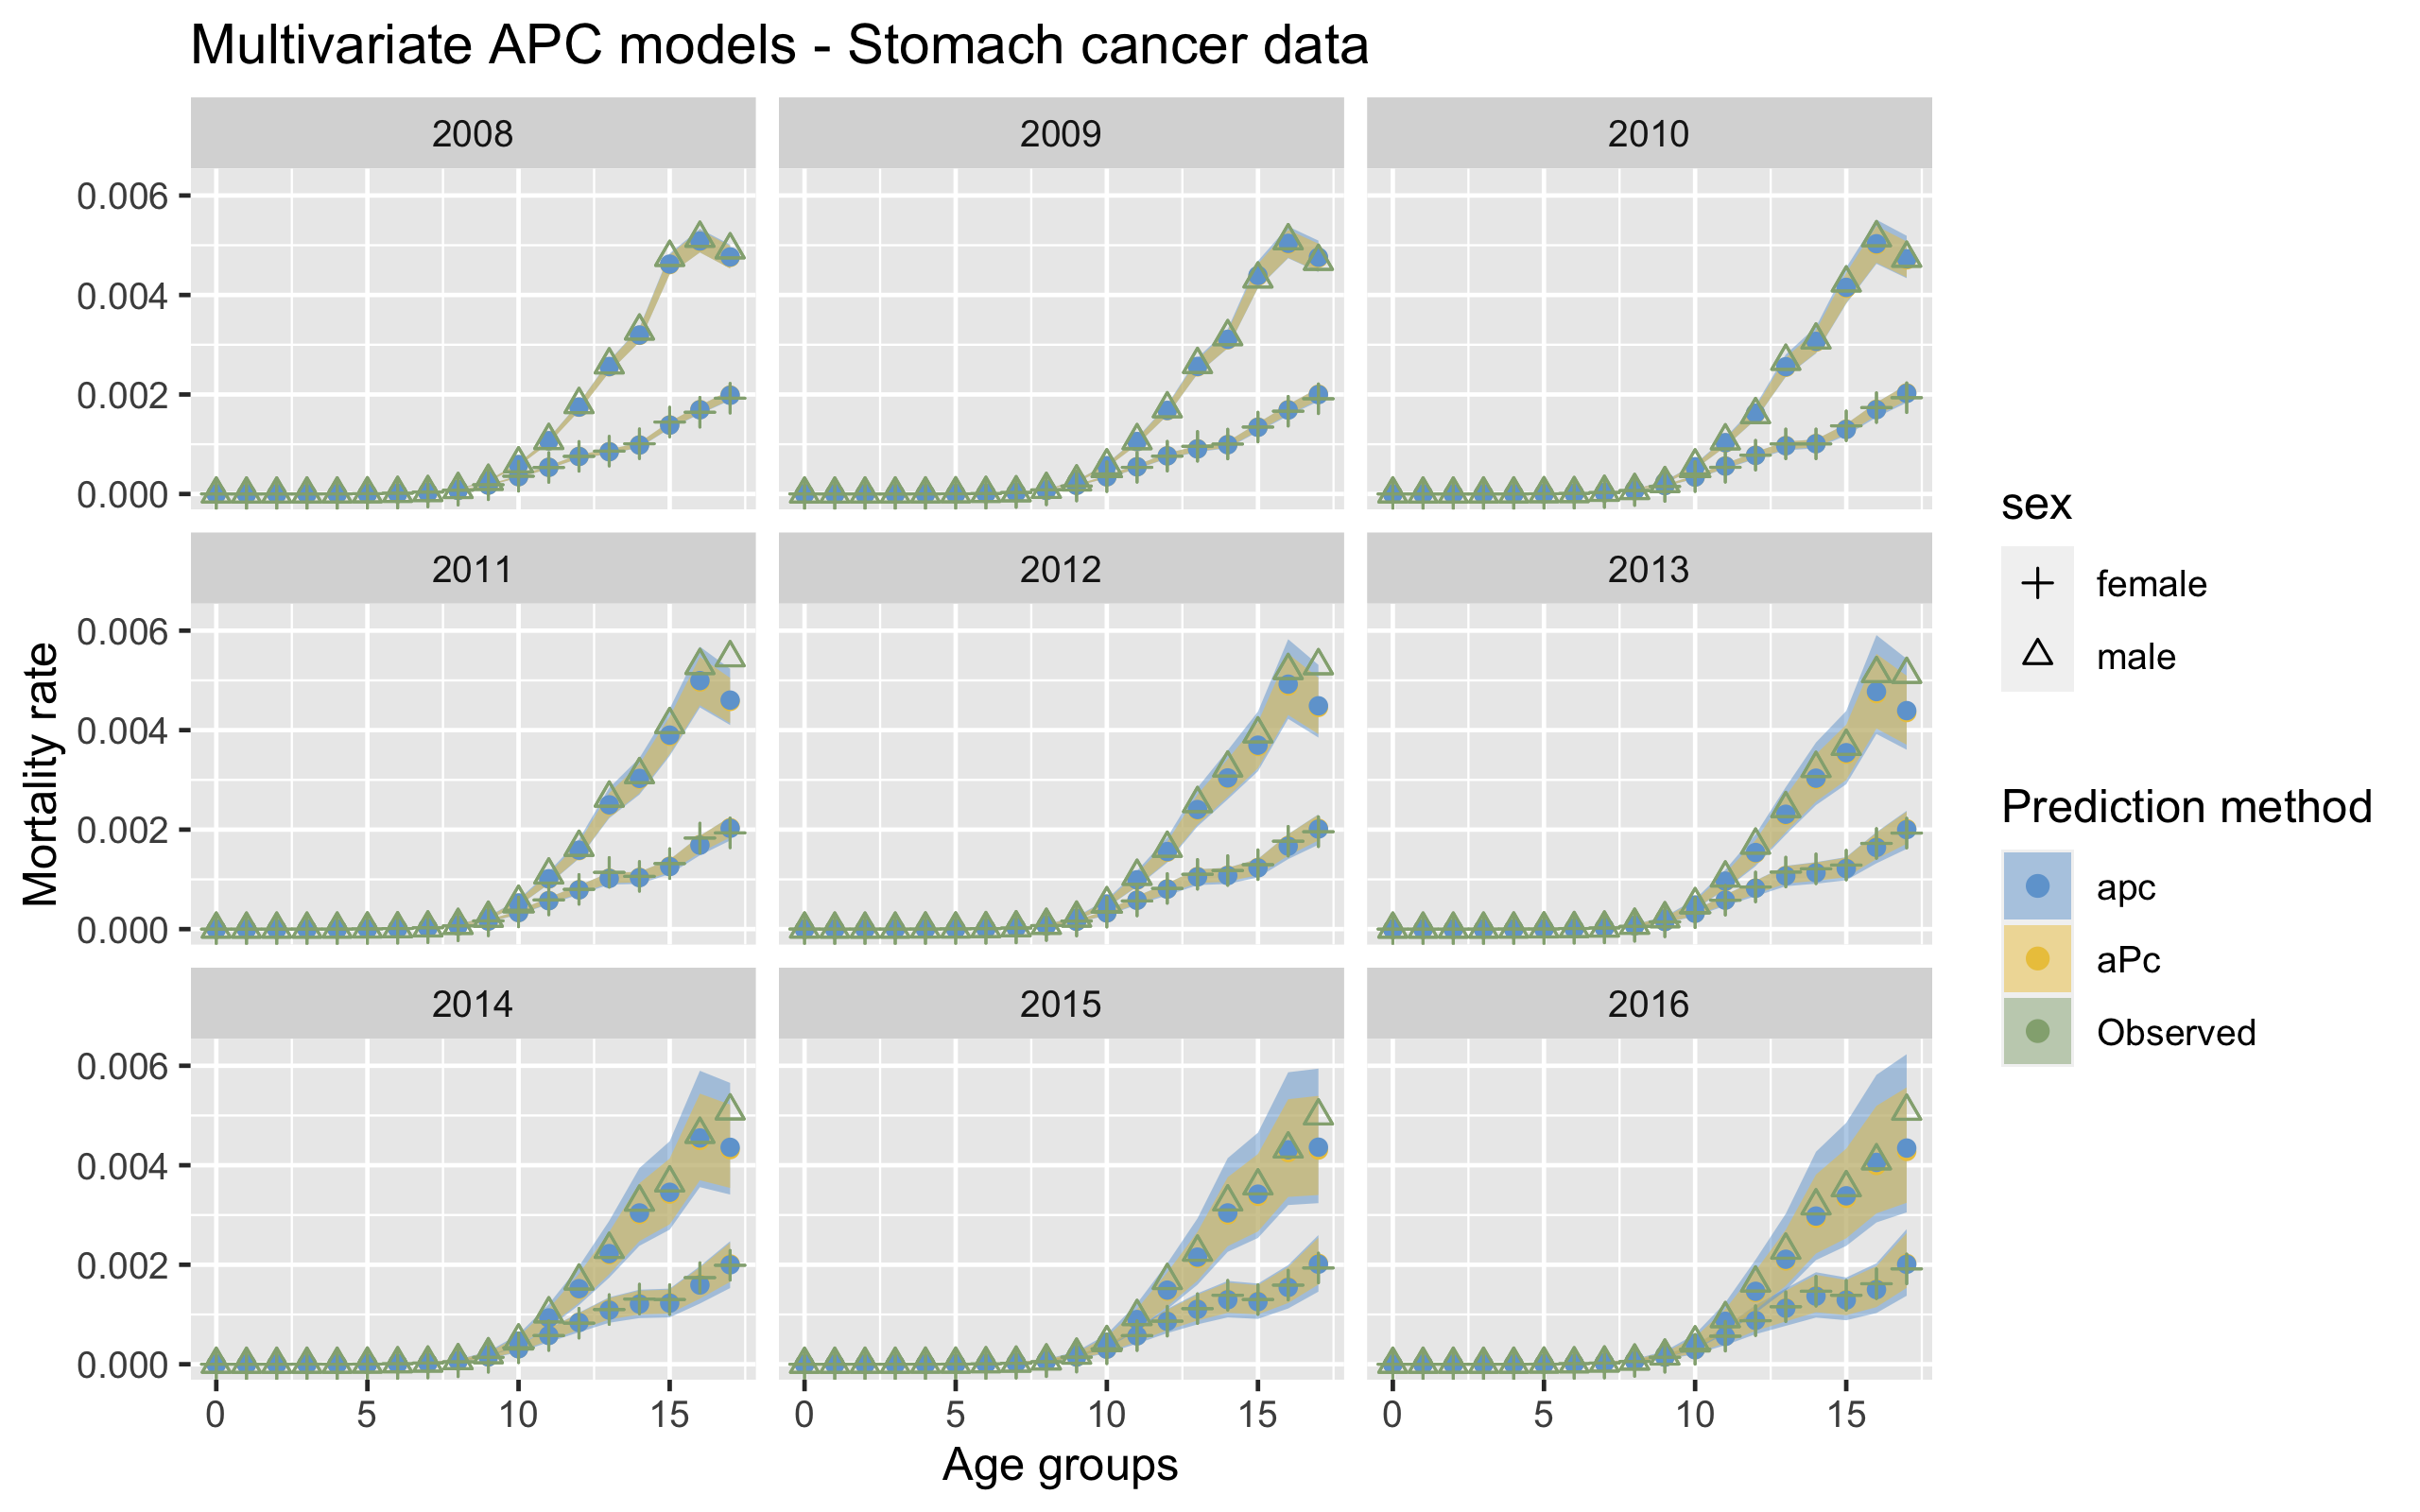
\includegraphics[width=\linewidth]{real-data/real-data-multivariate/Figures/multivariate-APC-by-age-stomach.png}
    \end{subfigure}
    \begin{subfigure}[b]{.45\linewidth}
        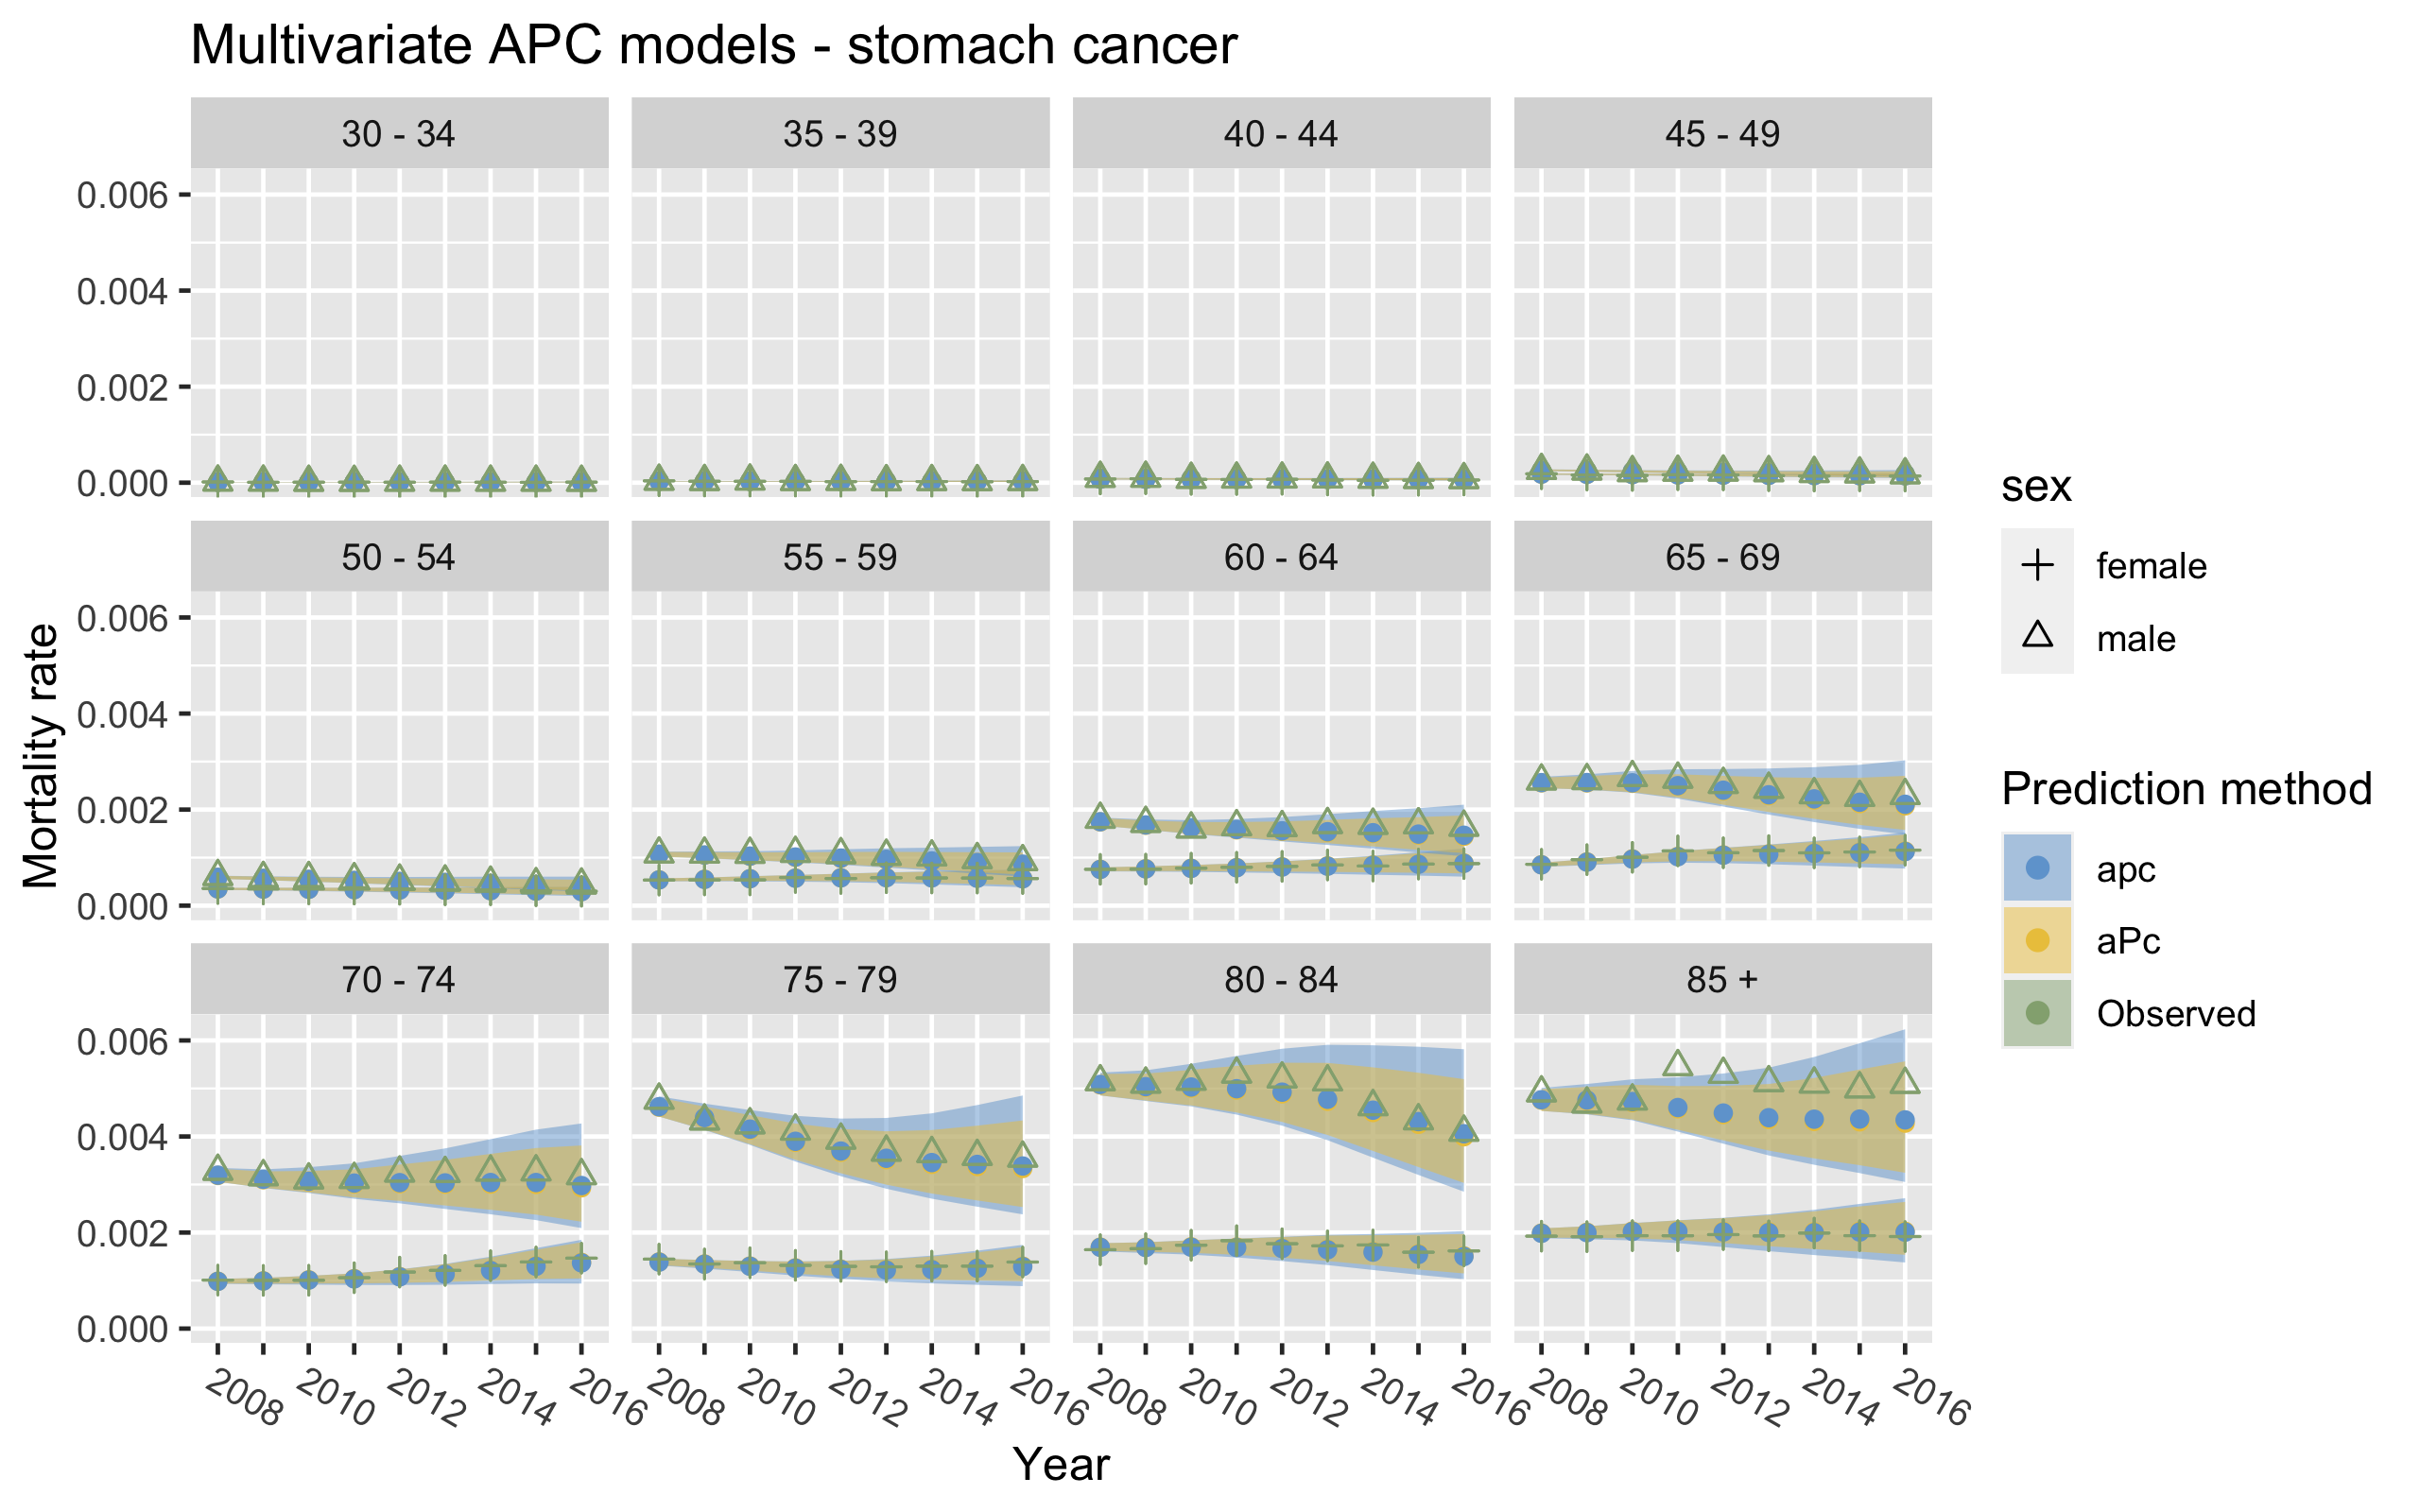
\includegraphics[width=\linewidth]{real-data/real-data-multivariate/Figures/multivariate-APC-by-period-stomach.png}
    \end{subfigure}
    \caption{The two best APC models - by age (left) and period (right) for the stomach cancer data set}
    \label{fig:mv-APC-stomach}
\end{figure}

\begin{figure}[h!]
    \centering
    \begin{subfigure}[b]{.45\linewidth}
        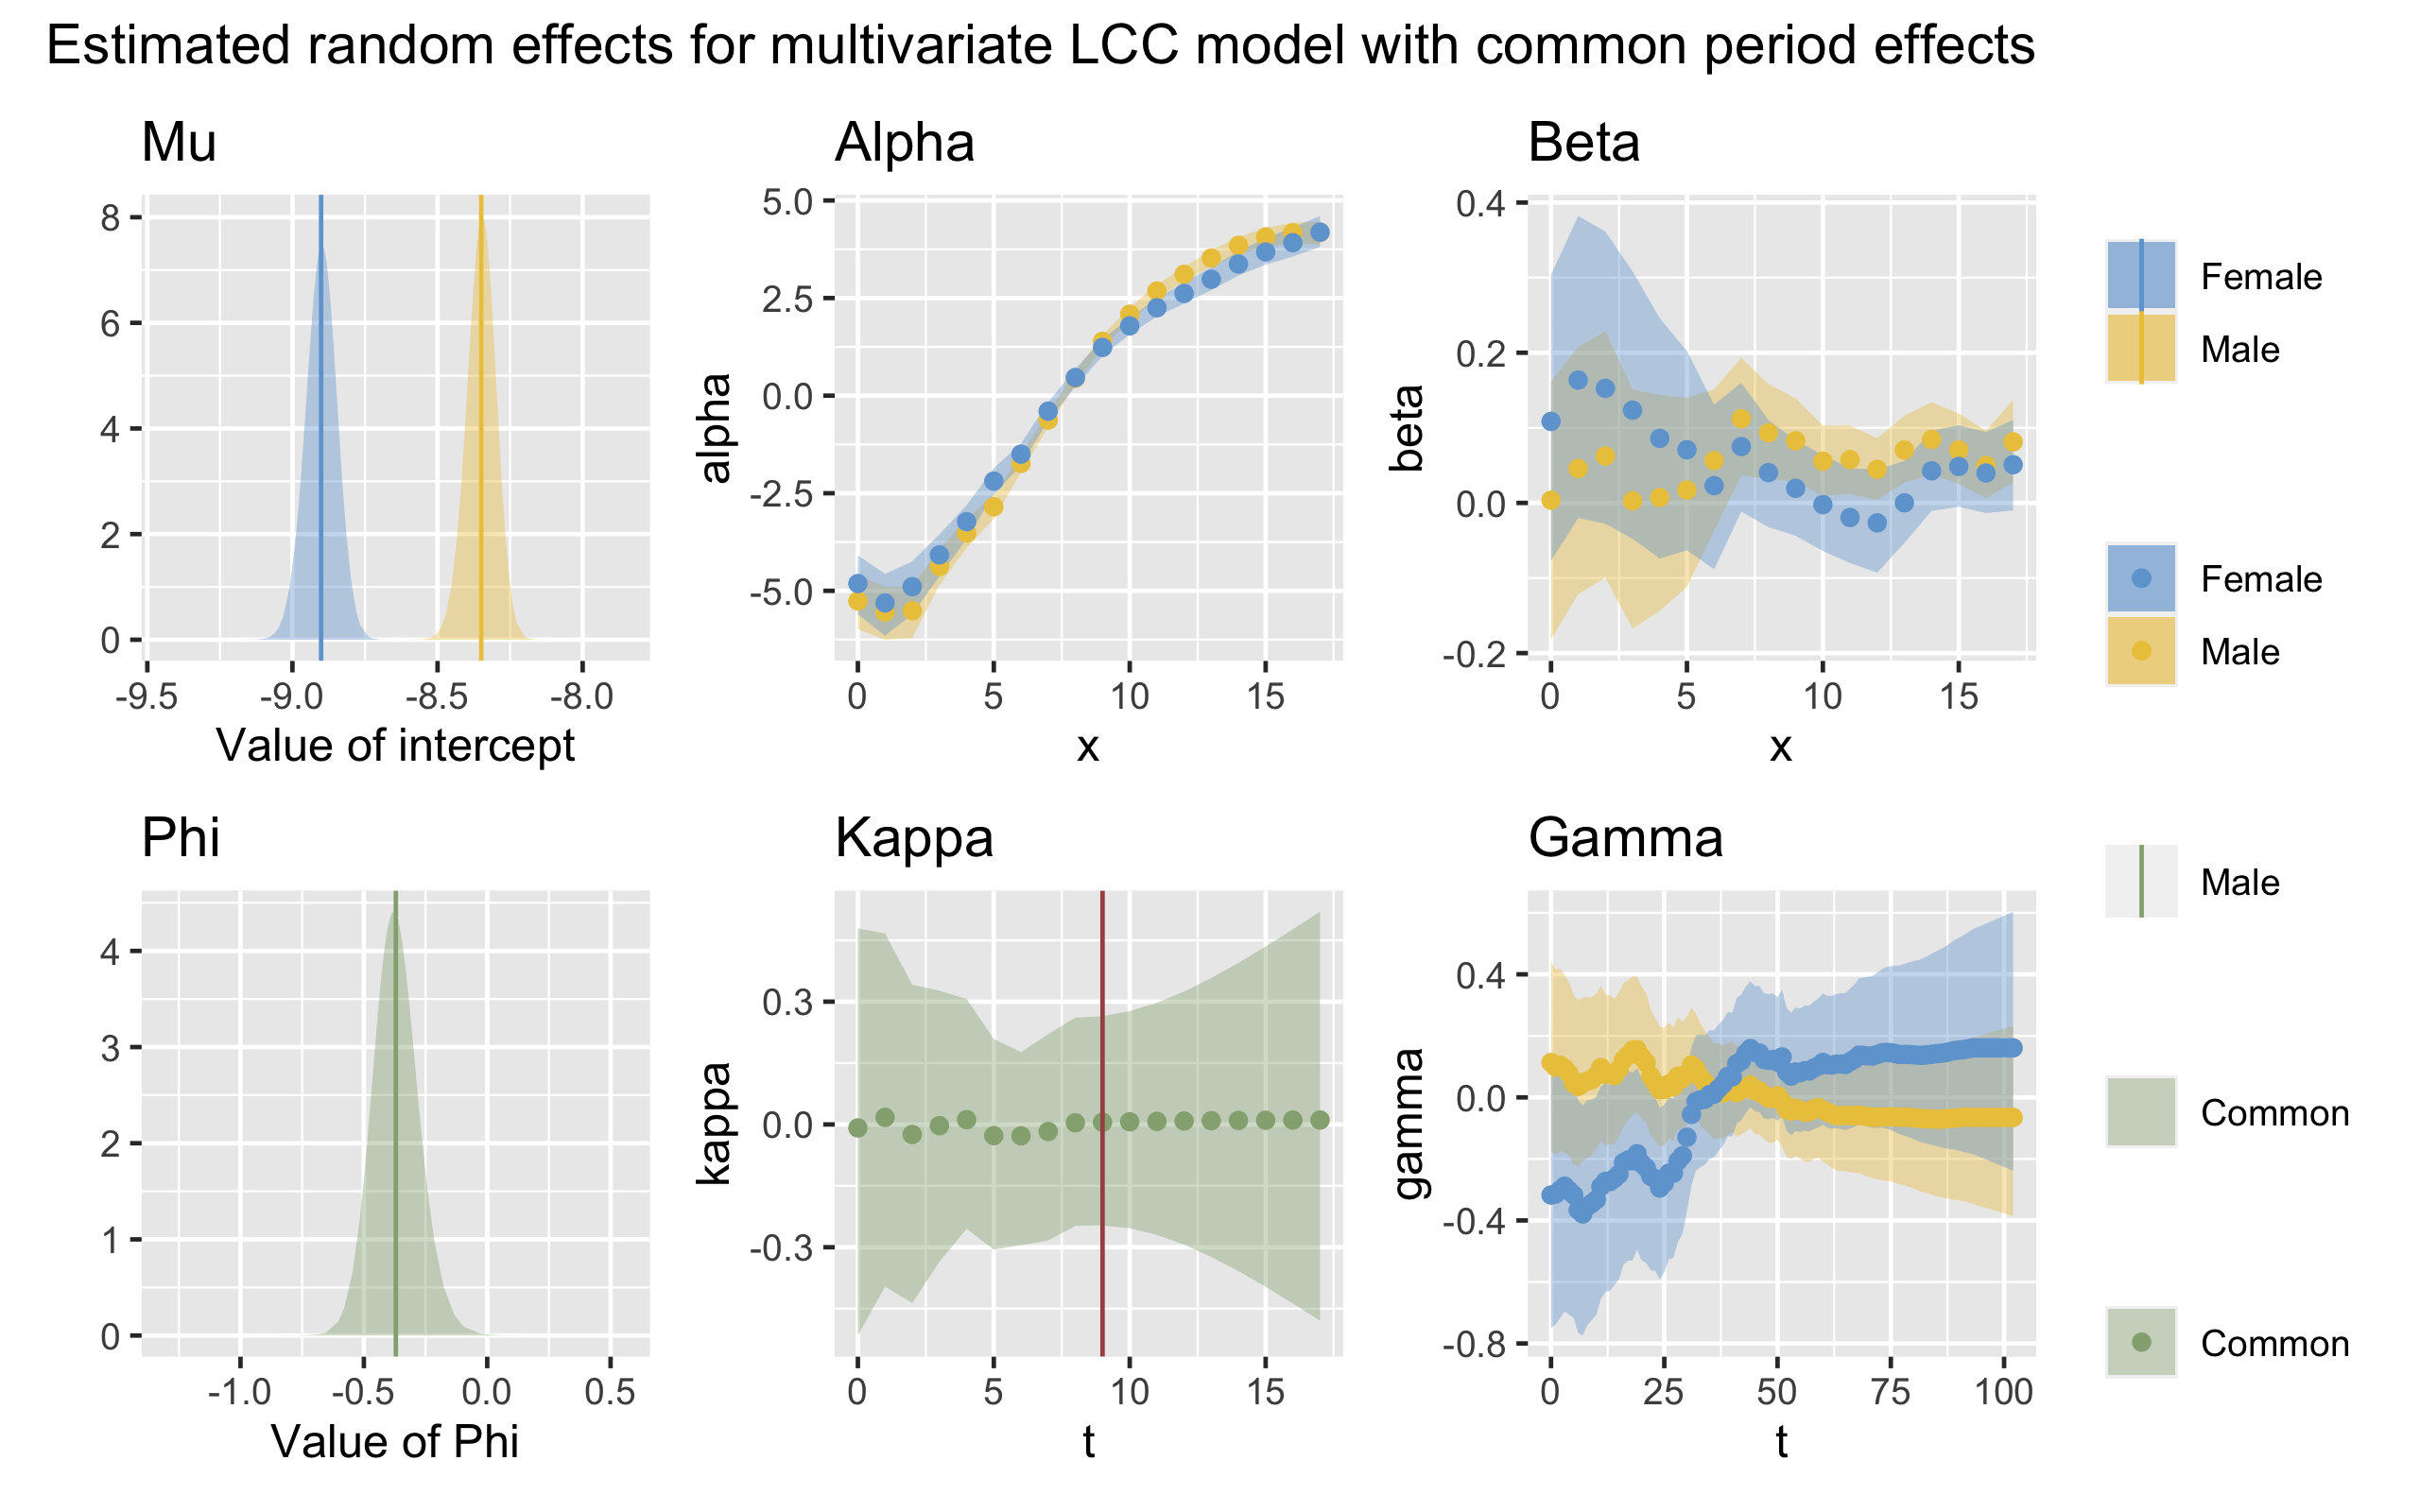
\includegraphics[width=\linewidth]{real-data/real-data-multivariate/Figures/effects-LCC-common-period-stomach.png}
    \end{subfigure}
    \begin{subfigure}[b]{.45\linewidth}
        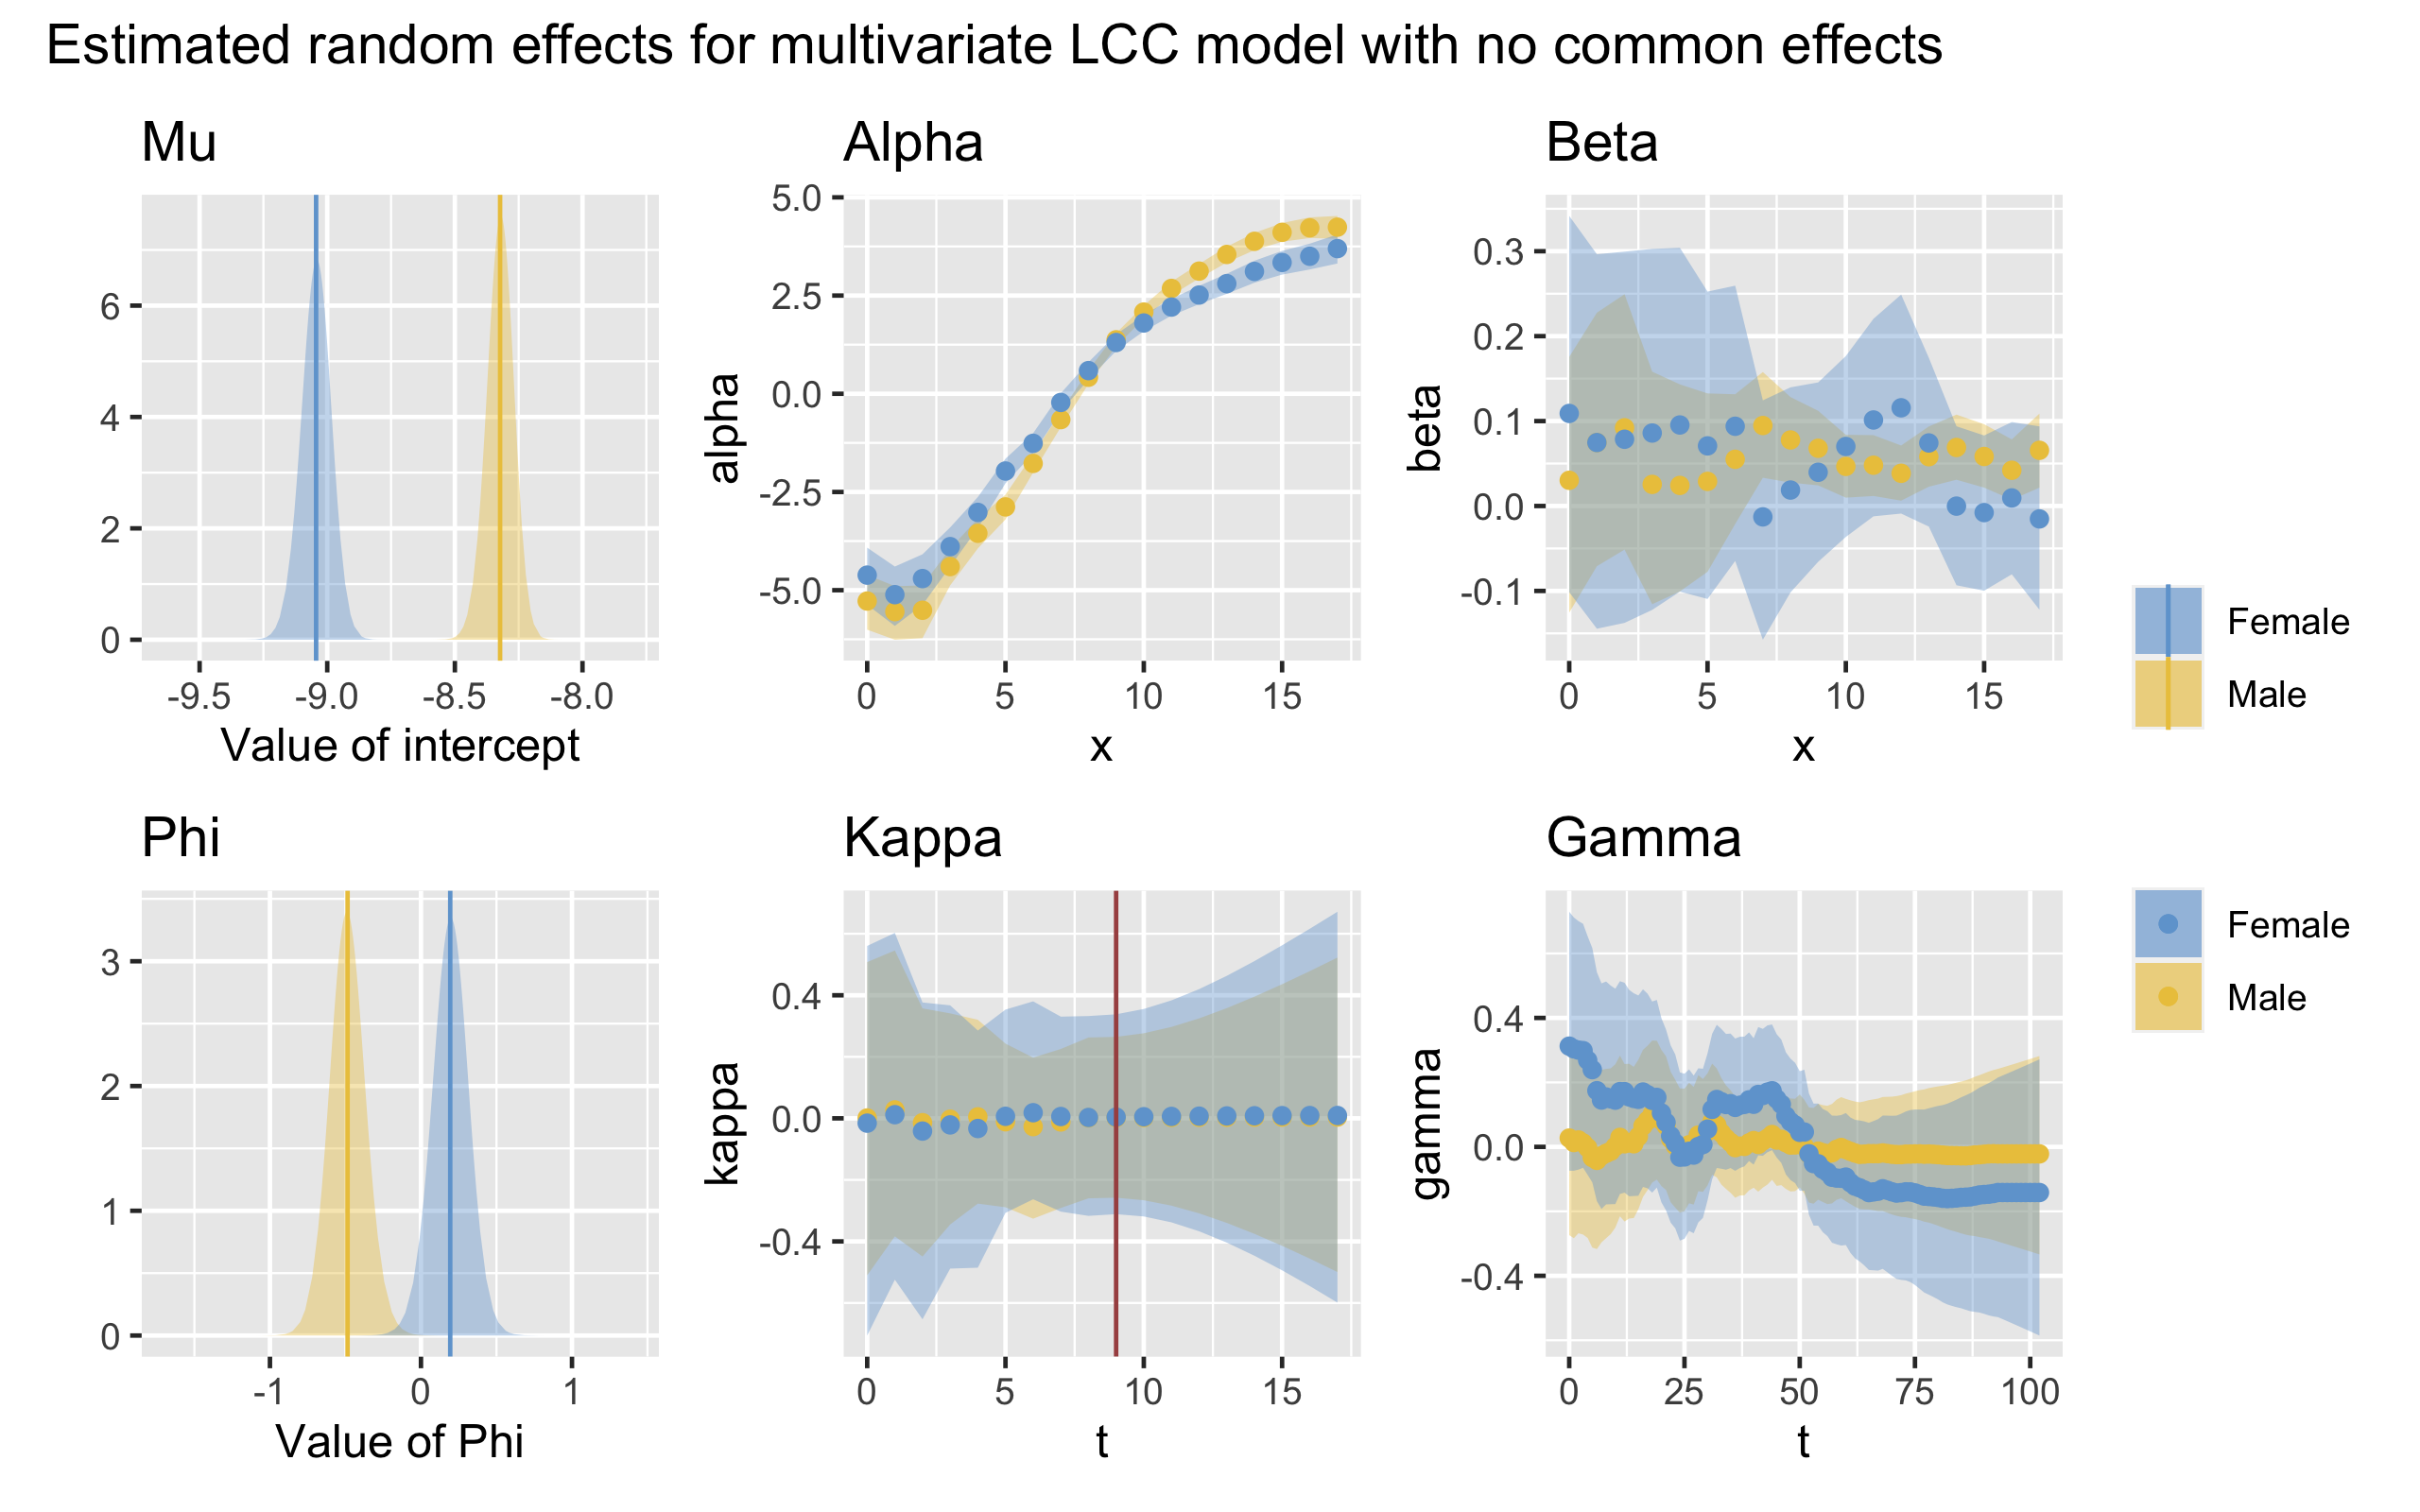
\includegraphics[width=\linewidth]{real-data/real-data-multivariate/Figures/effects-LCC-no-common-stomach.png}
    \end{subfigure}
    \caption{Plots of the effects for the two best LCC models - LCC with common period effects (left) and LCC with no common effects (right) for the lung cancer data}
    \label{fig:effects-LCC-stomach}
\end{figure}

\begin{figure}[h!]
    \centering
    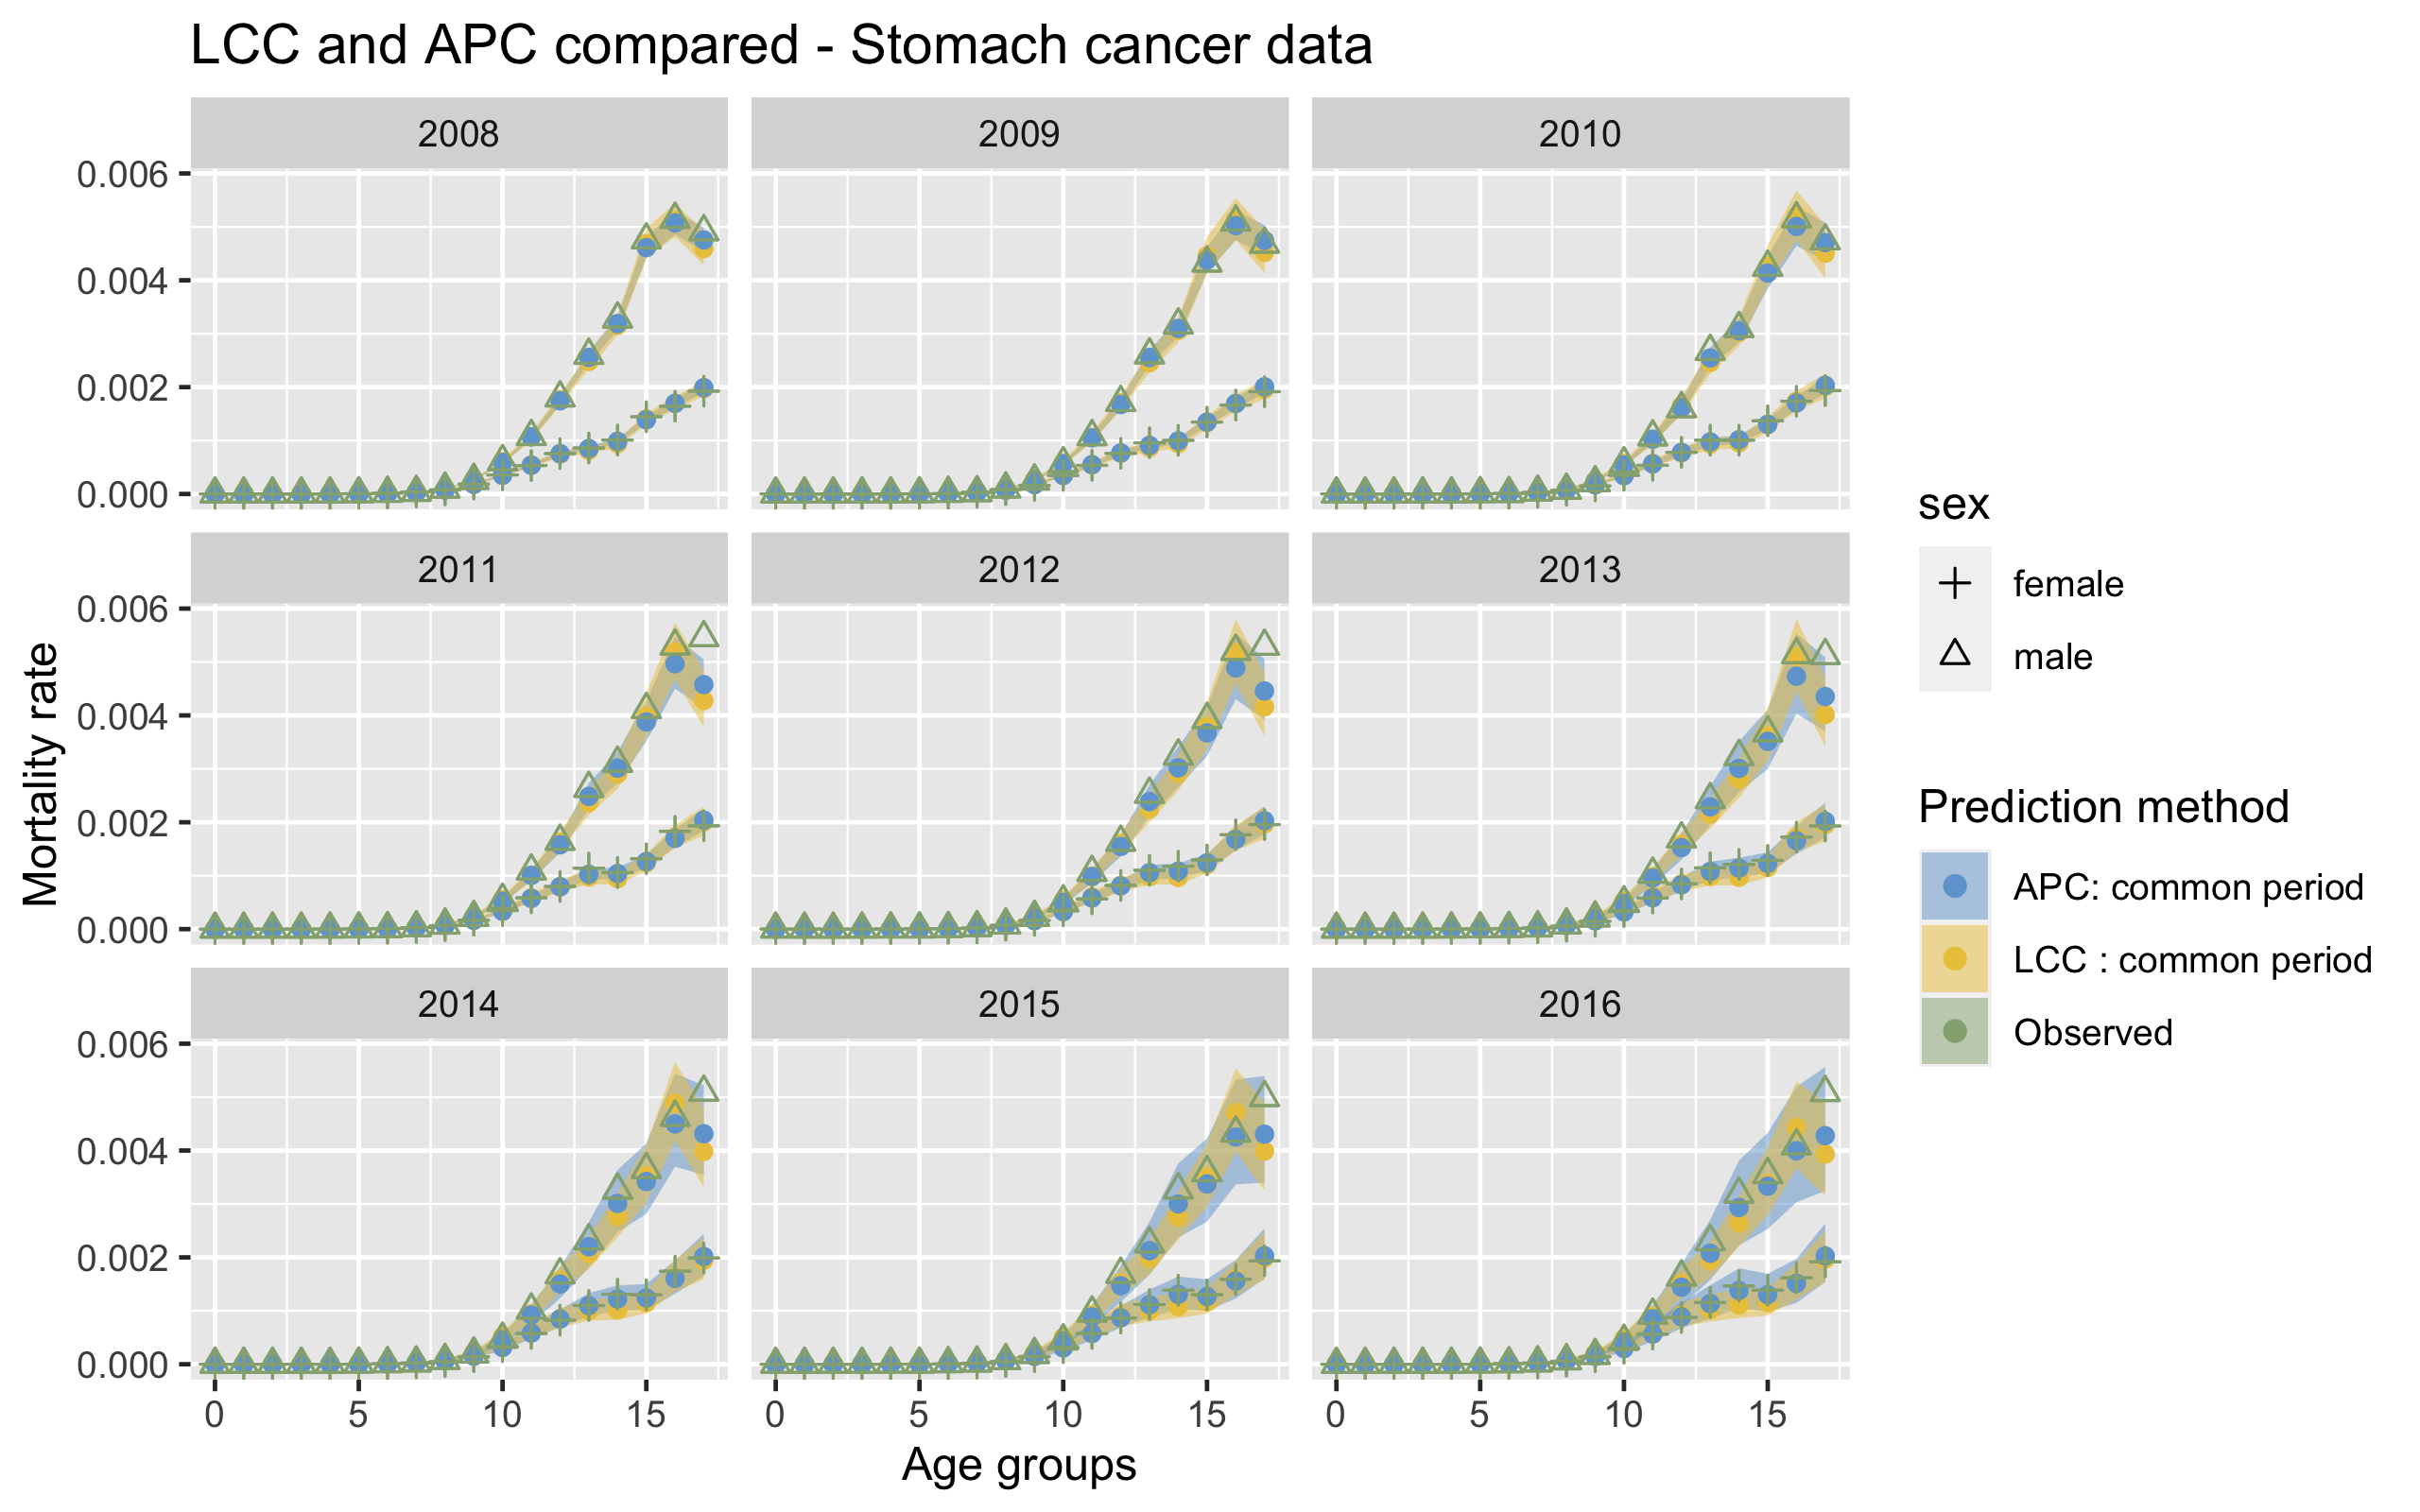
\includegraphics[width = .8\linewidth]{real-data/real-data-multivariate/Figures/multivariate-comparison-by-age-stomach.png}
    \caption{Comparison of the best APC model and the best LCC model - by age, for the stomach cancer data set. }
    \label{fig:mv-LCC-by-period-stomach}
\end{figure}

\begin{figure}[h!]
    \centering
    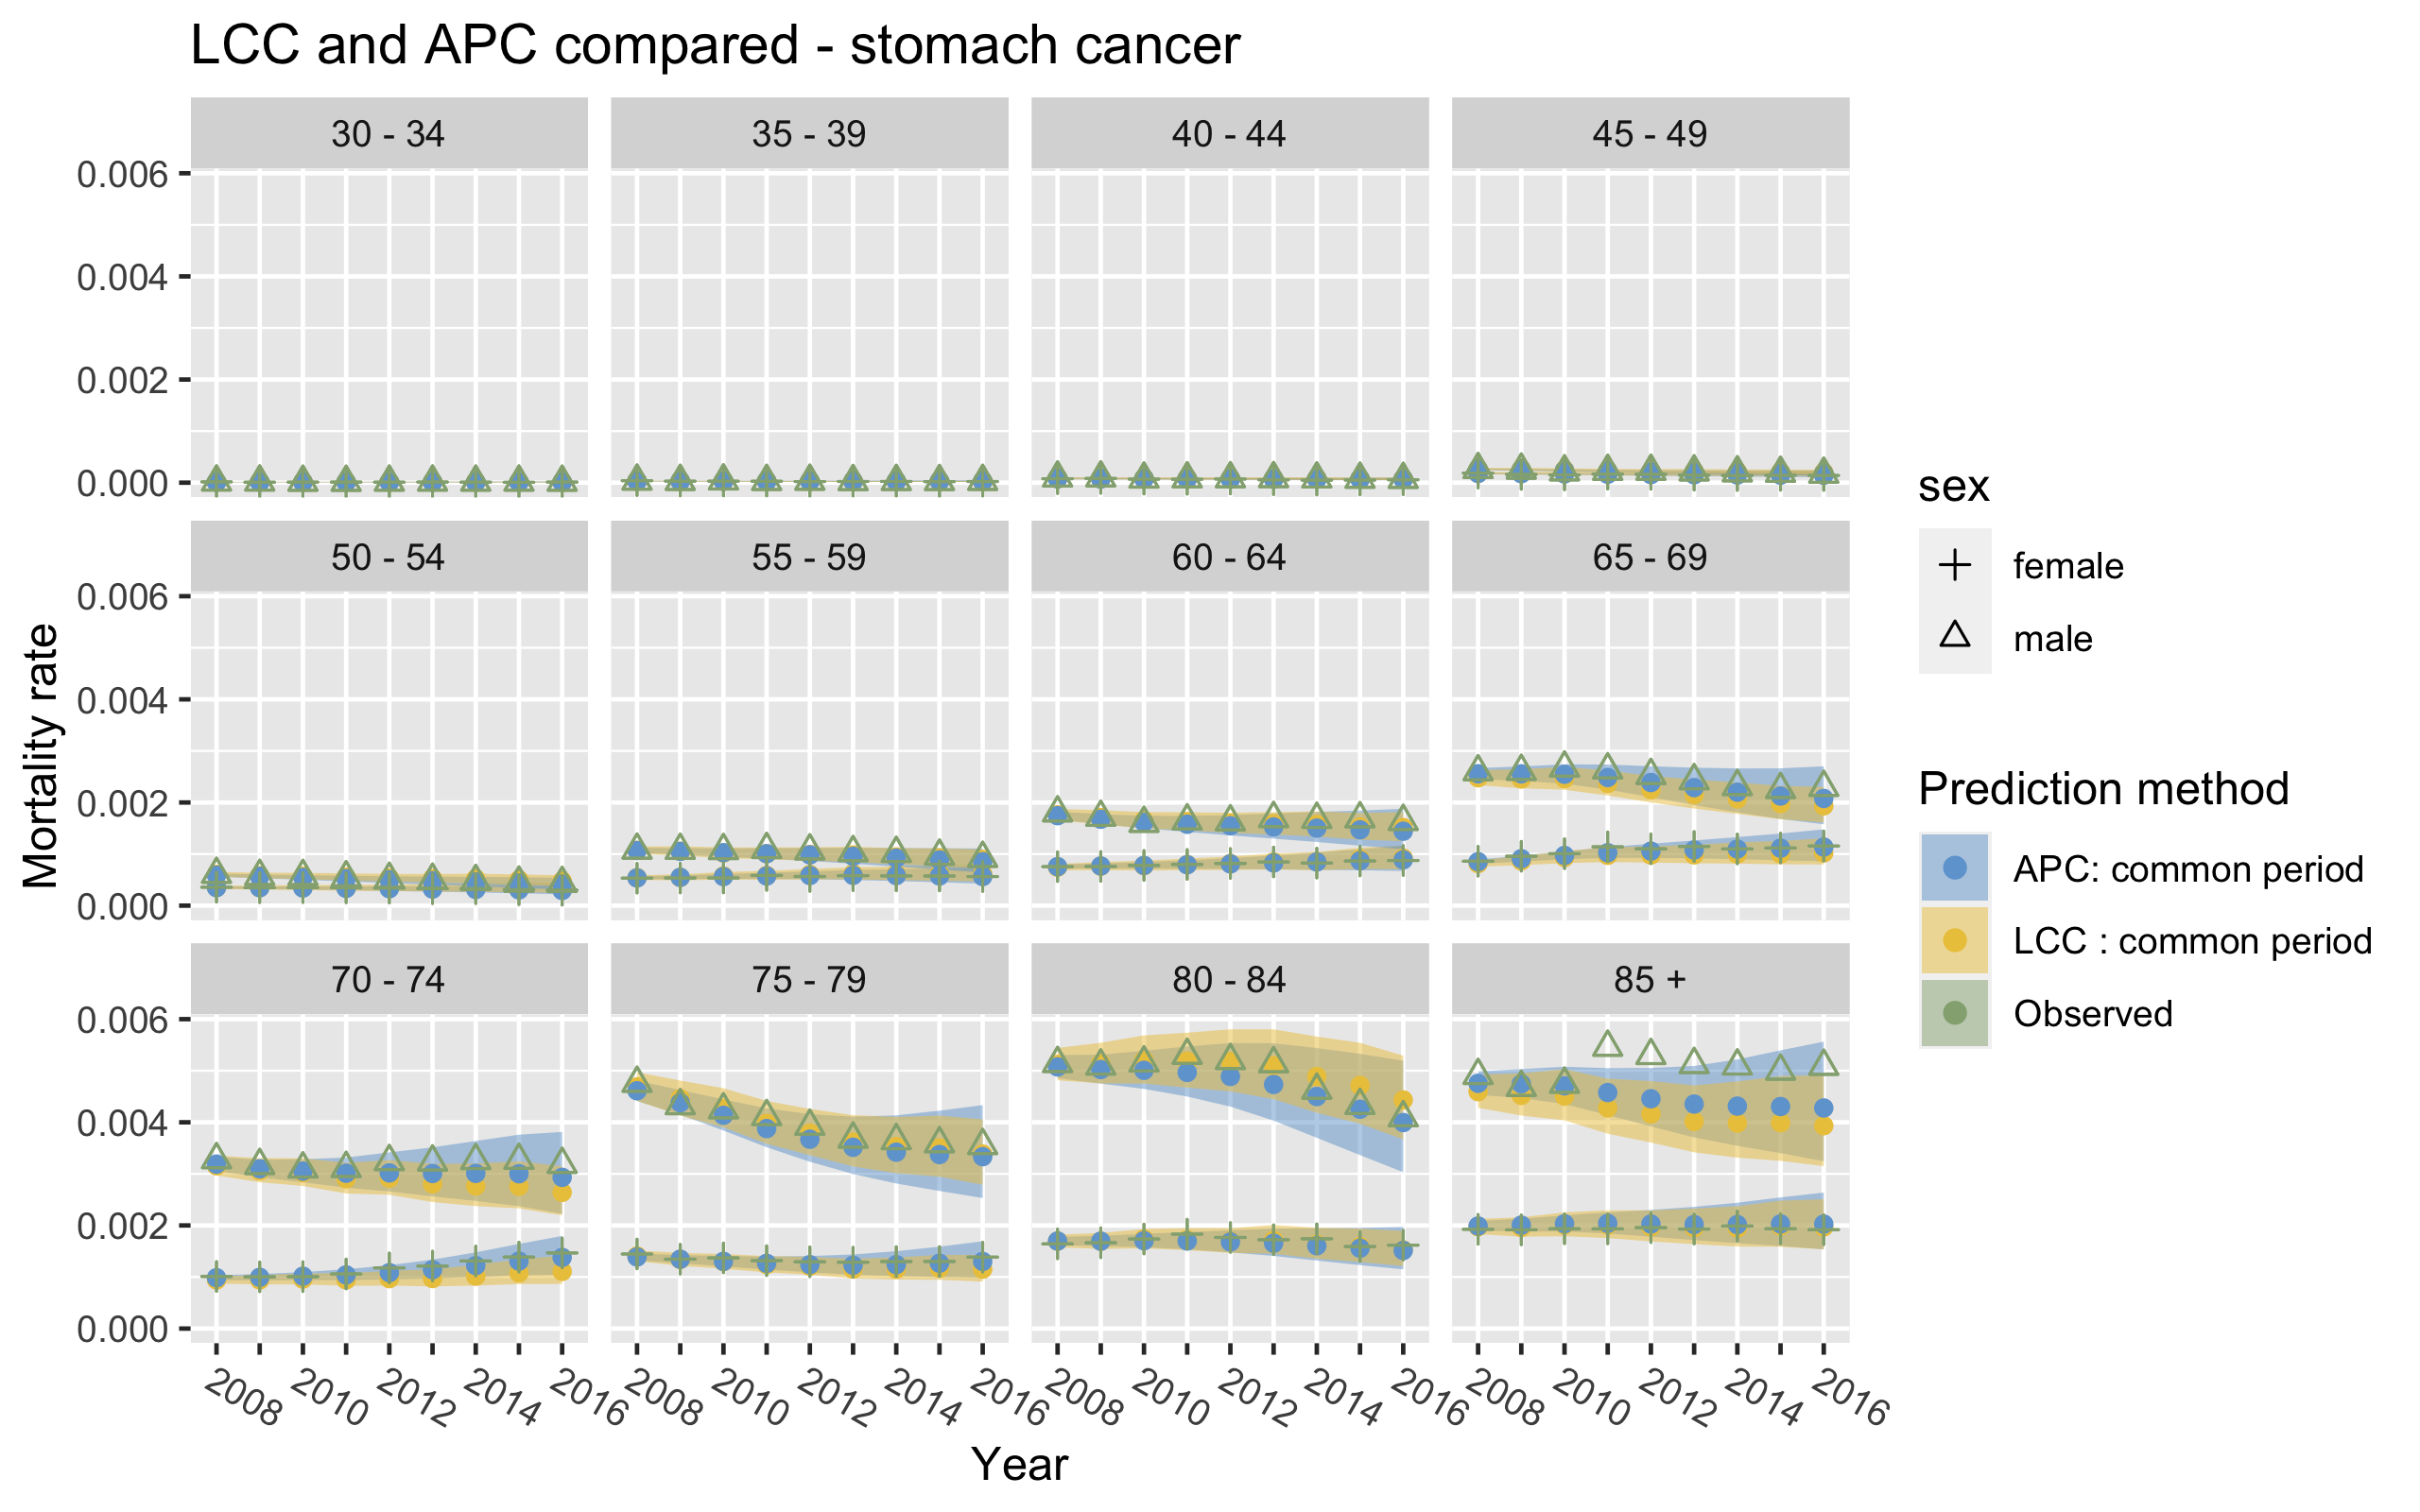
\includegraphics[width = .8\linewidth]{real-data/real-data-multivariate/Figures/multivariate-comparison-by-period-stomach.png}
    \caption{Comparison of the best APC model and the best LCC model - by period, for the stomach cancer data set}
    \label{fig:mv-APC-by-period-stomach}
\end{figure}

\newpage
\subsection{Sensitivity analysis}
\textcolor{myDarkGreen}{Skriv om behovet for en sensitivity analysis - så langt har du bare valgt relativt lite informative priors, uten å legge vekt på dette valget. Undersøk om man får forskjellig resultat av å endre prior for hyperparametrene. Presenter hvilke nye priors du tester. Presenter score statistics for forskjellige priors. 
Understrek at du ser veldig liten forskjell, og konkluderer med at valget ditt av priors sannsynligvis ikke påvirket resultatet i stor grad. 
\newline
Figurer:
\begin{itemize}
    \item Plott av forskjellige priors sammen - gir et tydelig bilde på hvor stor endringen er mellom de forskjellige priorene. 
\end{itemize}}

\begin{figure}[h!]
    \centering
    \begin{subfigure}[b]{.45\linewidth}
        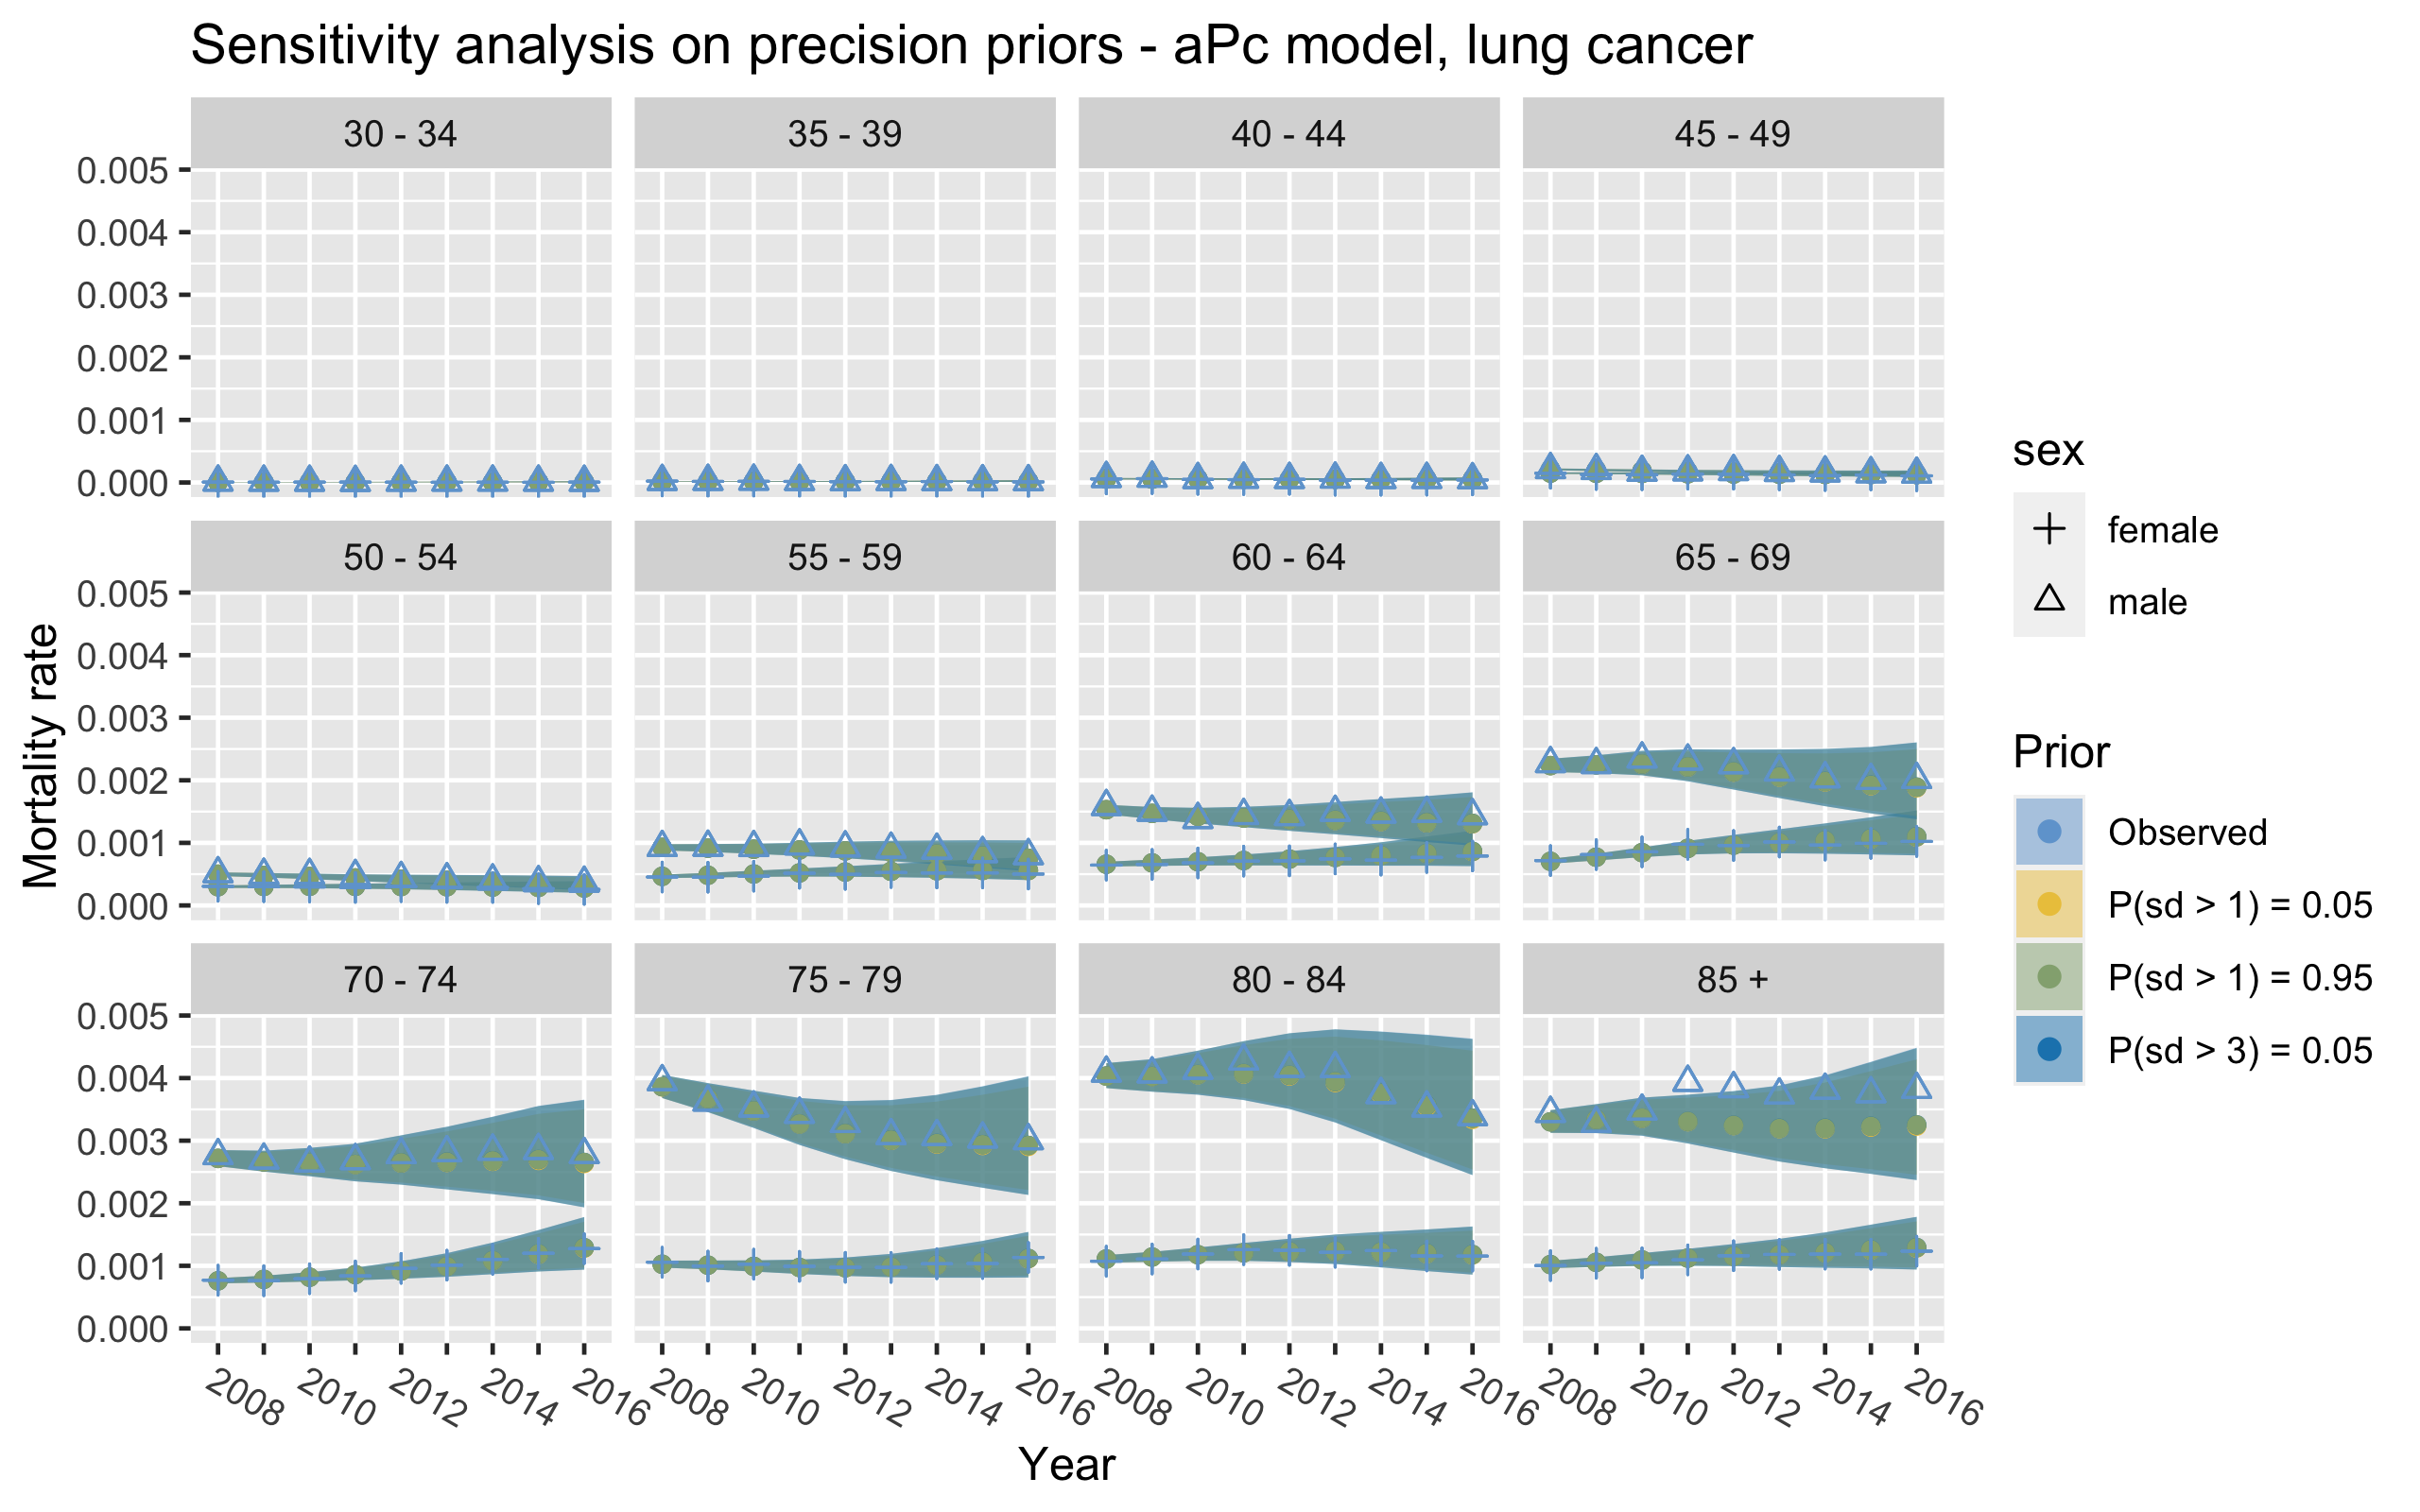
\includegraphics[width=\linewidth]{real-data/real-data-multivariate/Figures/sensitivity-analysis-aPc-by-period-lung.png}
    \end{subfigure}
    \begin{subfigure}[b]{.45\linewidth}
        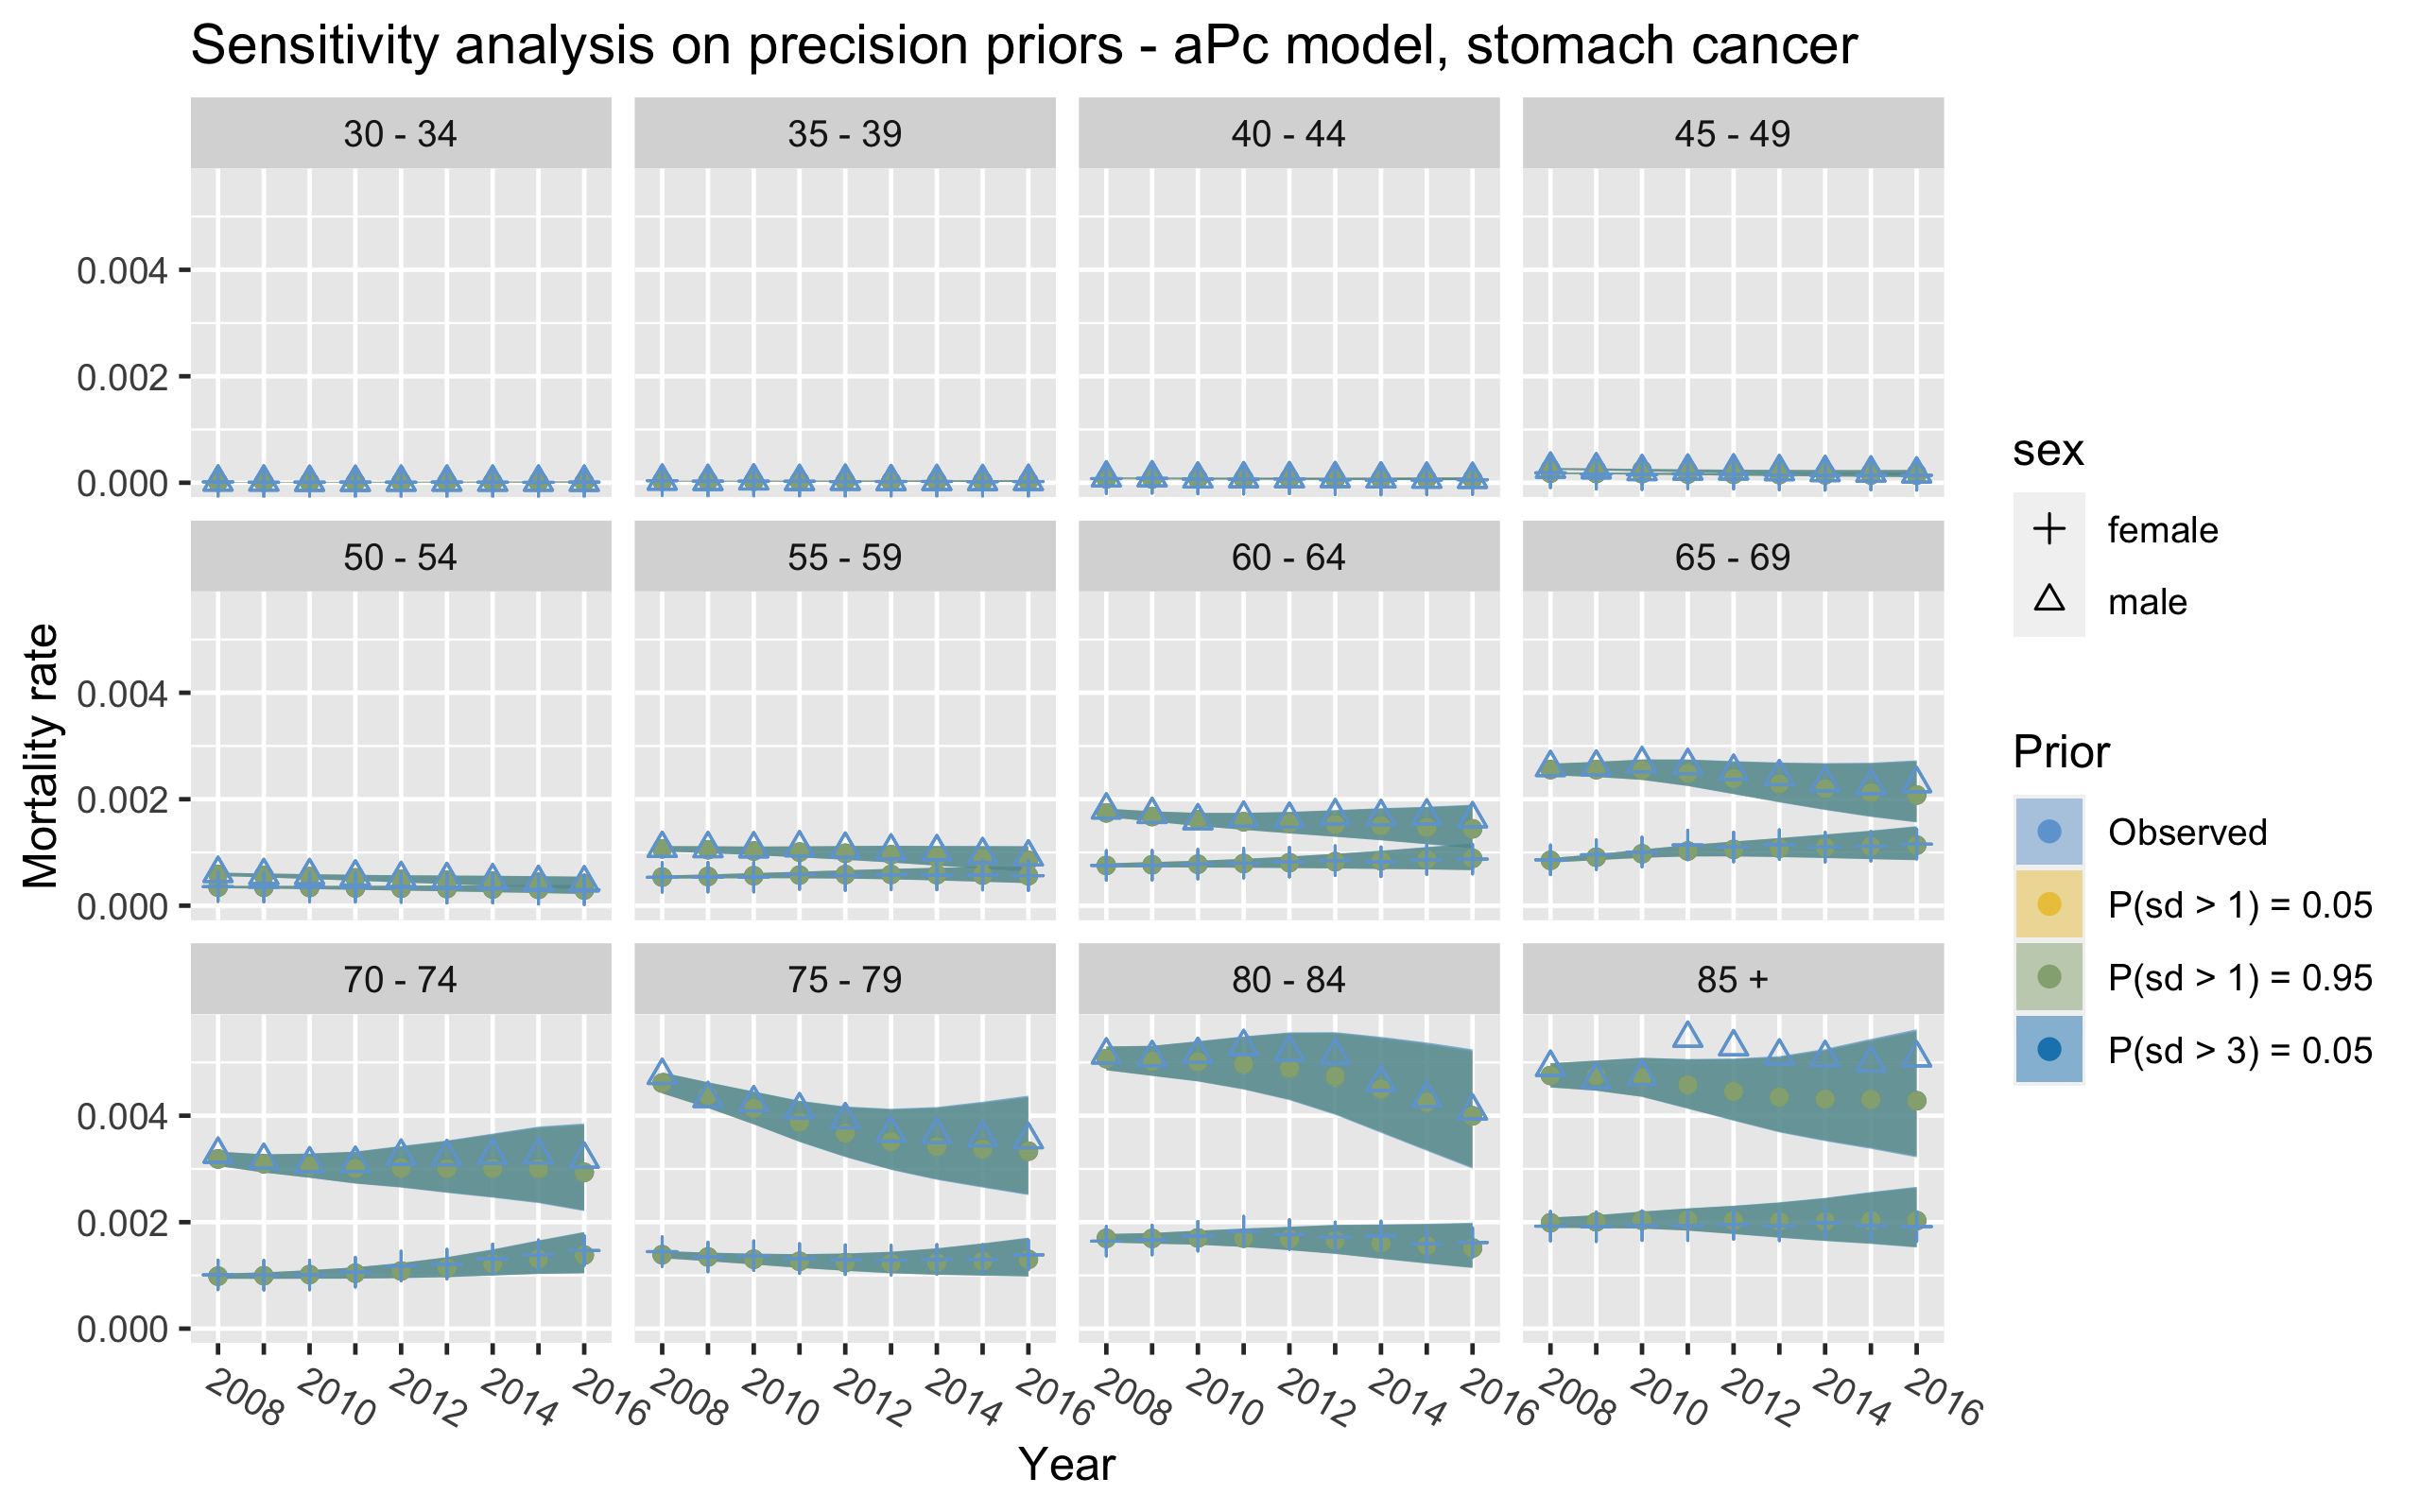
\includegraphics[width=\linewidth]{real-data/real-data-multivariate/Figures/sensitivity-analysis-aPc-by-period-stomach.png}
    \end{subfigure}
    \caption{Results from sensitivity analysis of the model that displayed the best predctive performance for lung cancer, the aPc-model (left), and stomach cancer, also the aPc model (right). }
    \label{fig:mv-sensitivity}
\end{figure}

\newpage 
\subsection{Identifiability issues}
\textcolor{myDarkGreen}{
Here, you can mention apparent identifiability issues. Perhaps talk about periodicity in cohort effects? Mention that a linear kappa might have been sufficient. 
}

\newpage 
\newpage
\newpage
\subsection{Old version - might still be parts that we want to use}
% change name of the section 
We test the previously described models on data containing deaths by lung- and stomach cancer, respectively, in Germany for the years 1999-2016. The observations are grouped by age groups of five years. We use the \inlabru library to run different versions of the LC- and APC models, and compare them. To be able to compare the performance of the different models, we omit the observations for year 2015 and 2016 and use the model fitted to the remaining data to predict the mortality rate for these two years. 

\subsection{LC and LCC on full dataset}
To get an overview of the dataset and the performance of the LC model on these datasets, we begin by fitting the LC and the LCC model to the full datasets and compare it to plots of the data. 

Figures \ref{fig:data-by-age}, \ref{fig:data-by-year} and \ref{fig:data-by-cohort} display percent-wise deaths by lung - and stomach cancer, by age groups, years and cohorts (birth years) respectively. Figure \ref{fig:LC-full-dataset} display the random effects obtained by fitting the LC-model to the two data sets, as well as the estimated predictor. Figure \ref{fig:LCC-full-dataset} displays the results from fitting the LCC-model to the stomach cancer data set. 

\begin{figure}[h!]
    \centering
    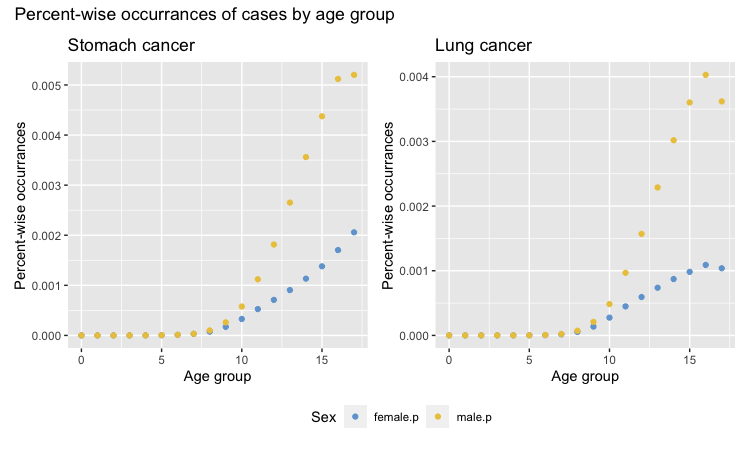
\includegraphics[width = .9\linewidth]{Figures/Results/Data/data-by-age-percent.png}
    \caption{The full stomach and lung cancer data sets, plotted by age groups $x = 0,\ldots,17$, for all years. }
    \label{fig:data-by-age}
\end{figure}

\begin{figure}[h!]
    \centering
    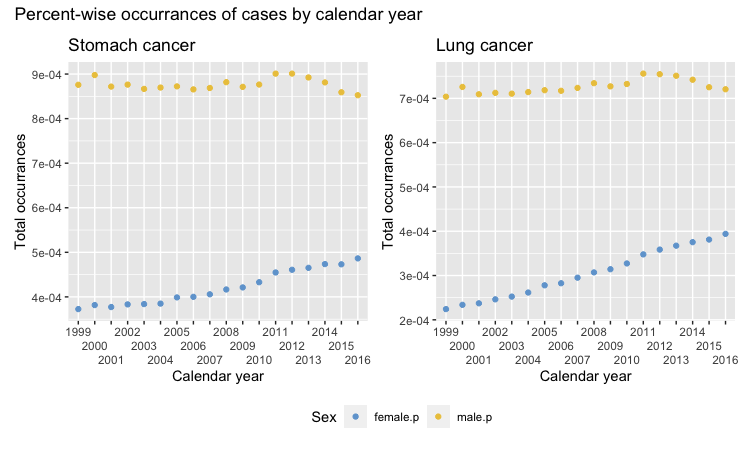
\includegraphics[width = .9\linewidth]{Figures/Results/Data/data-by-year-percent.png}
    \caption{The full stomach and lung cancer data sets, plotted for each year, for all ages. }
    \label{fig:data-by-year}
\end{figure}

\begin{figure}[h!]
    \centering
    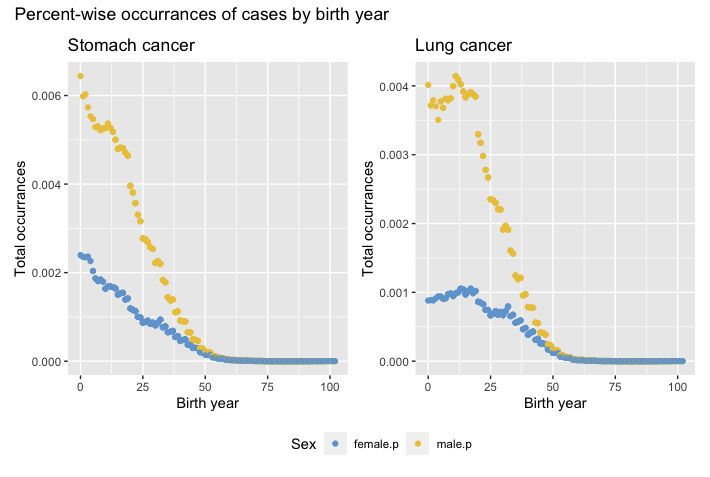
\includegraphics[width = .9\linewidth]{Figures/Results/Data/data-by-cohort-percent.png}
    \caption{The full stomach and lung cancer data sets, plotted for each cohort $k = 0,\ldots,102$, for all ages and years.}
    \label{fig:data-by-cohort}
\end{figure}


\begin{figure}[h!]
    \centering
    \begin{subfigure}[b]{.45\linewidth}
        \includegraphics[width=\linewidth]{Figures/Runs/Runs - real data/16.03:1341/16.03:1341 Alpha.png}
    \end{subfigure}
    \begin{subfigure}[b]{.45\linewidth}
        \includegraphics[width=\linewidth]{Figures/Runs/Runs - real data/16.03:1341/16.03:1341 Kappa.png}
    \end{subfigure}
    
    \centering
    \begin{subfigure}[b]{.45\linewidth}
        \includegraphics[width=\linewidth]{Figures/Runs/Runs - real data/16.03:1341/16.03:1341 Beta.png}
    \end{subfigure}
    \begin{subfigure}[b]{.45\linewidth}
        \includegraphics[width=\linewidth]{Figures/Runs/Runs - real data/16.03:1341/16.03:1341 Phi.png}
    \end{subfigure}
    
    \centering
    \begin{subfigure}[b]{.45\linewidth}
        \includegraphics[width=\linewidth]{Figures/Runs/Runs - real data/16.03:1341/16.03:1341 Eta t.png}
    \end{subfigure}
    \begin{subfigure}[b]{.45\linewidth}
        \includegraphics[width=\linewidth]{Figures/Runs/Runs - real data/16.03:1341/16.03:1341 Eta x.png}
    \end{subfigure}

    \caption{The LC-model applied both to the stomach cancer data and lung cancer data, with no absent values. }
    \label{fig:LC-full-dataset}
\end{figure}

\begin{figure}[h!]
\centering
\begin{subfigure}[b]{.3\linewidth}
    \includegraphics[width=\linewidth]{Figures/Runs/Runs - real data/16.03:1326/16.03:1326 Alpha.png}
\end{subfigure}
\begin{subfigure}[b]{.3\linewidth}
    \includegraphics[width=\linewidth]{Figures/Runs/Runs - real data/16.03:1326/16.03:1326 Kappa.png}
\end{subfigure}
\begin{subfigure}[b]{.3\linewidth}
    \includegraphics[width=\linewidth]{Figures/Runs/Runs - real data/16.03:1326/16.03:1326 Beta.png}
\end{subfigure}

\centering
\begin{subfigure}[b]{.3\linewidth}
    \includegraphics[width=\linewidth]{Figures/Runs/Runs - real data/16.03:1326/16.03:1326 Gamma.png}
\end{subfigure}
\begin{subfigure}[b]{.3\linewidth}
    \includegraphics[width=\linewidth]{Figures/Runs/Runs - real data/16.03:1326/16.03:1326 Eta t.png}
\label{fig:26.02:1607 Gamma}
\end{subfigure}
\begin{subfigure}[b]{.3\linewidth}
    \includegraphics[width=\linewidth]{Figures/Runs/Runs - real data/16.03:1326/16.03:1326 Eta x.png}
\label{fig:26.02:1607 Eta}
\end{subfigure}

\centering
\begin{subfigure}[b]{.3\linewidth}
    \includegraphics[width=\linewidth]{Figures/Runs/Runs - real data/16.03:1326/16.03:1326 Phi.png}
\label{fig:LCC-full-dataset}
\end{subfigure}

\caption{The LCC model applied to the stomach cancer data set. }
\label{fig:26.02:1607}
\end{figure}

From the Figure \ref{fig:LC-full-dataset} and Figure \ref{fig:LCC-full-dataset} we see that $\alphav$ is the random effect that is modeled with the highest precision for both the LC-model and the LCC-model. This indicates a clear tendency of change in the mortality rate for different age groups, with a higher mortality rate for older age groups. Figure \ref{fig:data-by-age} confirms this, as it shows a much higher mortality rate for older age groups, for both males and females. 
We observe from Figures \ref{fig:LC-full-dataset} and \ref{fig:LCC-full-dataset} that there is much higher uncertainty related to the estimation of the period effects, $\kappav$ and $\phi\cdot t$. The estimated $\kappav$ seemes in both cases to be almost insignificant, with wide confidence bounds centered around zero. The $\phi \cdot t$ effect on the other hand, does show a clear tendency of a decreasing mortality rate for higher years. [TODO: TENK GJENNOM HVORFOR PHI ER NEGATIV NÅR DU HAR EN ØKENDE TIDSTREND!! HER KAN DU JO BEGYNNE Å SPEKULERE I AT DET KANSKJE ER SMART Å HA MED EN KOHORT-EFFEKT...] We also observe a clear tendency in the cohort-effects. [OGSÅ: LEGG TIL NYE PLOTT AV EFFEKT MED LC PÅ EKTE DATA, TROR DE DU HAR NÅ KAN VÆRE UTDATERTE..]

\subsection{Prediction using LC-models}
So far, we have discussed two different versions of the Lee-Carter model, the original LC-model and the LCC-model, which is extended by a cohort effect. Considering the results from above, where we observed that the $\kappav$ effect did not seem to be significant, it is reasonable to also consider a third version of the LC model, where we only use the $\phi \cdot t$ factor to model period effects:
\begin{equation}
    \etax = \mu + \alphax + \betax\cdot\phi\cdot t + \gammax + \epsilon_{x,t}.
    \label{eq:LClinear}
\end{equation}
We compare the performance of these three models by fitting these models to the data sets with missing values for the years 2015 and 2016, and then using these models to predict the missing mortality rates. This way, we are able to assess the performance of the different models compared to each other and say something about which model is the preferred model in our case. 

\begin{figure}
    \centering
    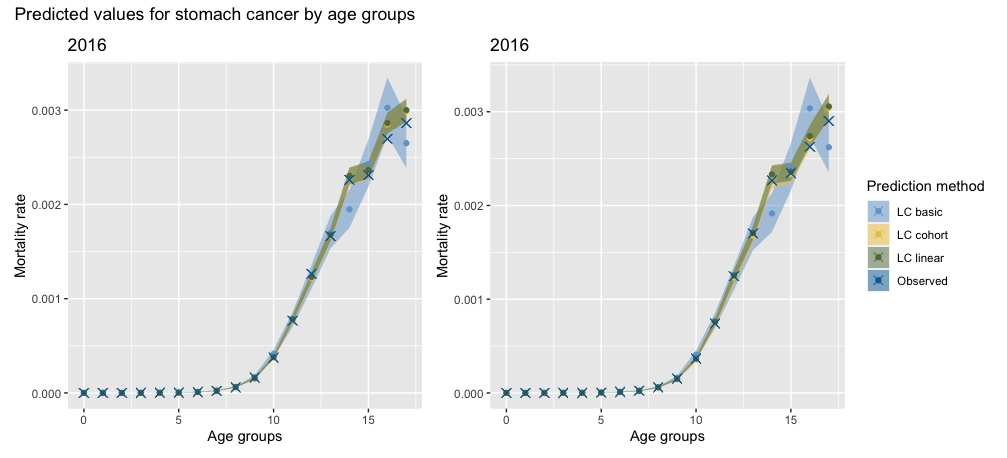
\includegraphics[width = .9\linewidth]{Figures/Results/LC-pred-compare-agex-s.png}
    \caption{The predicted mortality rates of stomach cancer for 2015 (left) and 2016 (right) from three different versions of the LC-model: the basic LC-model (light blue), the LCC-model (yellow) and the LCC-model without the $\kappat$ factor (green), together with the observed mortality rates (dark blue crosses).}
    \label{fig:LC-compare-s}
\end{figure}

\begin{figure}
    \centering
    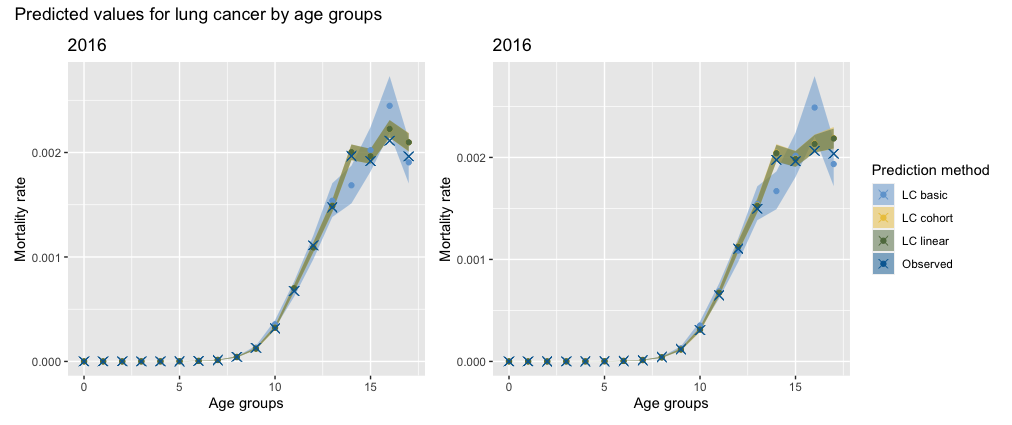
\includegraphics[width = .9\linewidth]{Figures/Results/LC-pred-compare-lung-ageX.png}
    \caption{The predicted mortality rates of lung cancer for 2015 (left) and 2016 (right) from three different versions of the LC-model: the basic LC-model (light blue), the LCC-model (yellow) and the LCC-model without the $\kappat$ factor (green), together with the observed mortality rates (dark blue crosses).}
    \label{fig:LC-compare-l}
\end{figure}

From Figures \ref{fig:LC-compare-l} and \ref{fig:LC-compare-s} it is clear that the basic LC-model is less suited to predict the mortality rates for older age groups for both stomach cancer patients and lung cancer patients. The two remaining models, the LCC-model and the LCC-model with only a linear period effect seem to give more or less equally accurate and precise predictions. When running \inlabru for these two models, we observe that the script using the LCC-model takes quite a while longer to converge. Since Figures \ref{fig:LC-compare-l} and \ref{fig:LC-compare-s} does not display any significant difference between the predictions of the two models, we can say that we prefer the reduced LCC-model, and we use this in the further prediction from this point. [RECONSIDER WHETHER YOU ACTUALLY WANT TO MAKE THIS CHOICE. ]

In a similar fashion we compare the two different APC-models, using a random walk of first and second order, respectively, to model the age-, period- and cohort effects. [YOU SHOULD HAVE MENTIONED AND WRITTEN DOWN THESE MODELS EARLIER. ] A comparison of the predictions of the morality rates for lung and stomach cancer in 2015 and 2016 yielded by the two models are presented in Figures \ref{fig:APC-compare-s} and \ref{fig:APC-compare-l}. We observe that the two models give very similar predictions, but that the rw2-model seem to be somewhat more accurate. [ALSO, THE RW2 MODEL IS A BIT MORE "CORRECT"? SOMETHING ABOUT THIS IN ANDREAS PAPER.]  

\begin{figure}[h!]
    \centering
    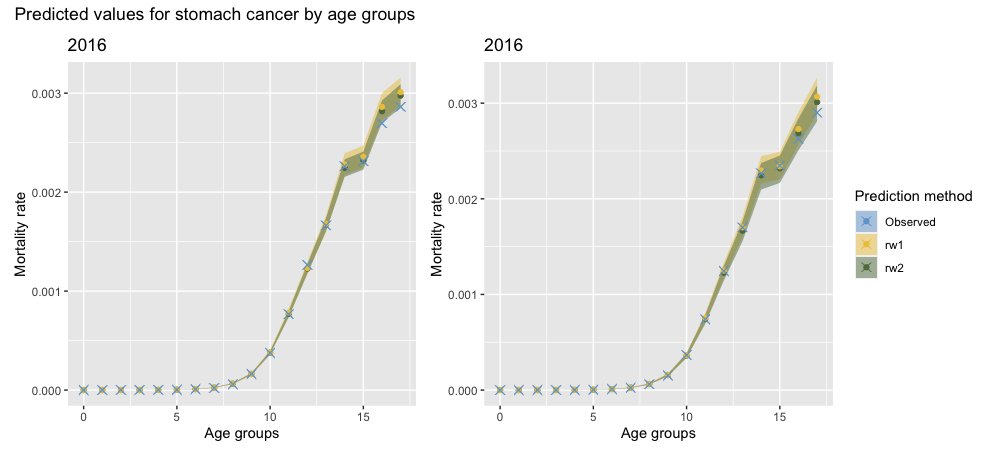
\includegraphics[width = .9\linewidth]{Figures/Results/pred-APC-compare-s-agex.png}
    \caption{The predicted mortality rates of stomach cancer for 2015 (left) and 2016 (right) from two different versions of the APC-model: using a random walk of first order (rw1) (yellow) and a random walk of second order (rw2) (green) to model the random effects, together with the observed mortality rates (light blue crosses).}
    \label{fig:APC-compare-s}
\end{figure}

\begin{figure}[h!]
    \centering
    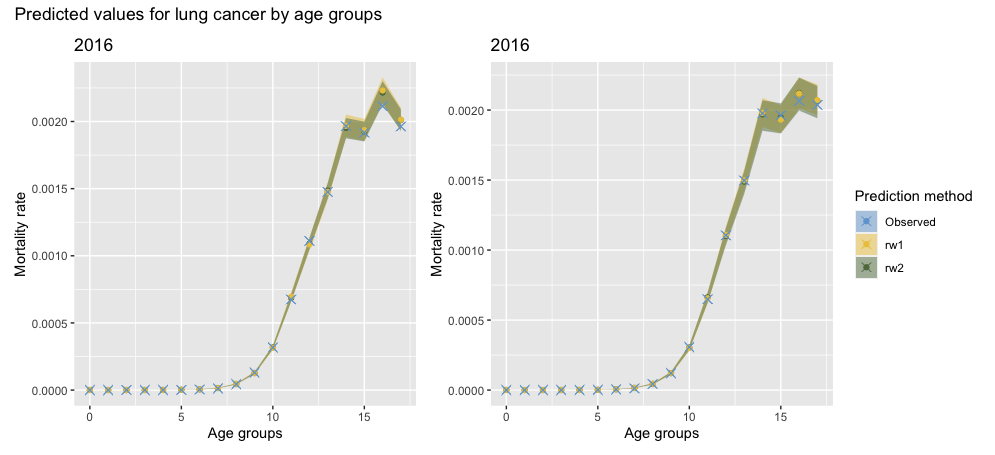
\includegraphics[width = .9\linewidth]{Figures/Results/pred-APC-comp-l-agex.png}
    \caption{The predicted mortality rates of lung cancer for 2015 (left) and 2016 (right) from two different versions of the APC-model: using a random walk of first order (rw1) (yellow) and a random walk of second order (rw2) (green) to model the random effects, together with the observed mortality rates (light blue crosses).}
    \label{fig:APC-compare-l}
\end{figure}

Finally, we compare the LC- and APC-models that yielded the best results - the LCC-model with a linear period-effect and the rw2 APC-model. The predictions are displayed in Figures \ref{fig:APC-LC-compare-s} and \ref{fig:APC-LC-compare-l}. We observe that the LCC and the APC models display quite simliar and good predictions of the mortality rates, but that the APC model predictions seem to be somewhat more precise than the LC model.

\begin{figure}[h!]
    \centering
    \includegraphics[width = .9\linewidth]{Figures/Results/pred-LC-APC-agex-s.png}
    \caption{The predicted mortality rates of stomach cancer for 2015 (left) and 2016 (right) for the rw2 APC-model (light blue) and the LCC-model with a linear period effect (yellow), together with the observed mortality rates (dark green crosses).}
    \label{fig:APC-LC-compare-s}
\end{figure}

\begin{figure}[h!]
    \centering
    \includegraphics[width = .9\linewidth]{Figures/Results/pred-LC-APC-agex-l.png}
    \caption{The predicted mortality rates of lung cancer for 2015 (left) and 2016 (right) for the rw2 APC-model (light blue) and the LCC-model with a linear period effect (yellow), together with the observed mortality rates (dark green crosses).}
    \label{fig:APC-LC-compare-l}
\end{figure}

Until now we have considered the performance of the predictions from the different models only graphically. Now, we will 